%https://www.overleaf.com/learn/latex/Subscripts_and_superscripts
\RequirePackage[2020-02-02]{latexrelease}
\documentclass[14pt,fleqn]{extbook} % Default font size and left-justified equations
\usepackage{graphicx}
\usepackage{setspace}
\usepackage{graphicx} % Required for including pictures
\graphicspath{{Pictures/}} % Specifies the directory where pictures are stored

\usepackage{lipsum} % Inserts dummy text

\usepackage{tikz} % Required for drawing custom shapes

\usepackage[english]{babel} % English language/hyphenation

\usepackage{enumitem} % Customize lists
\setlist{nolistsep} % Reduce spacing between bullet points and numbered lists

\usepackage{booktabs} % Required for nicer horizontal rules in tables

\usepackage{xcolor} % Required for specifying colors by name
\definecolor{ocre}{RGB}{243,102,25} % Define the orange color used for highlighting throughout the book

%----------------------------------------------------------------------------------------
%	MARGINS
%----------------------------------------------------------------------------------------

\usepackage{geometry} % Required for adjusting page dimensions and margins

\geometry{
	paper=a4paper, % Paper size, change to letterpaper for US letter size
	top=3cm, % Top margin
	bottom=3cm, % Bottom margin
	left=3cm, % Left margin
	right=3cm, % Right margin
	headheight=14pt, % Header height
	footskip=1.4cm, % Space from the bottom margin to the baseline of the footer
	headsep=10pt, % Space from the top margin to the baseline of the header
	%showframe, % Uncomment to show how the type block is set on the page
}

%----------------------------------------------------------------------------------------
%	FONTS
%----------------------------------------------------------------------------------------

\usepackage{avant} % Use the Avantgarde font for headings
%\usepackage{times} % Use the Times font for headings
\usepackage{mathptmx} % Use the Adobe Times Roman as the default text font together with math symbols from the Sym­bol, Chancery and Com­puter Modern fonts

\usepackage{microtype} % Slightly tweak font spacing for aesthetics
\usepackage[utf8]{inputenc} % Required for including letters with accents
\usepackage[T1]{fontenc} % Use 8-bit encoding that has 256 glyphs

%----------------------------------------------------------------------------------------
%	BIBLIOGRAPHY AND INDEX
%----------------------------------------------------------------------------------------

\usepackage[style=numeric,citestyle=numeric,sorting=nyt,sortcites=true,autopunct=true,babel=hyphen,hyperref=true,abbreviate=false,backref=true,backend=biber]{biblatex}
\addbibresource{bibliography.bib} % BibTeX bibliography file
\defbibheading{bibempty}{}

\usepackage{calc} % For simpler calculation - used for spacing the index letter headings correctly
\usepackage{makeidx} % Required to make an index
\makeindex % Tells LaTeX to create the files required for indexing

%----------------------------------------------------------------------------------------
%	MAIN TABLE OF CONTENTS
%----------------------------------------------------------------------------------------

\usepackage{titletoc} % Required for manipulating the table of contents

\contentsmargin{0cm} % Removes the default margin

% Part text styling (this is mostly taken care of in the PART HEADINGS section of this file)
\titlecontents{part}
	[0cm] % Left indentation
	{\addvspace{20pt}\bfseries} % Spacing and font options for parts
	{}
	{}
	{}

% Chapter text styling
\titlecontents{chapter}
	[1.25cm] % Left indentation
	{\addvspace{12pt}\large\sffamily\bfseries} % Spacing and font options for chapters
	{\color{ocre!60}\contentslabel[\Large\thecontentslabel]{1.25cm}\color{ocre}} % Formatting of numbered sections of this type
	{\color{ocre}} % Formatting of numberless sections of this type
	{\color{ocre!60}\normalsize\;\titlerule*[.5pc]{.}\;\thecontentspage} % Formatting of the filler to the right of the heading and the page number

% Section text styling
\titlecontents{section}
	[1.25cm] % Left indentation
	{\addvspace{3pt}\sffamily\bfseries} % Spacing and font options for sections
	{\contentslabel[\thecontentslabel]{1.25cm}} % Formatting of numbered sections of this type
	{} % Formatting of numberless sections of this type
	{\hfill\color{black}\thecontentspage} % Formatting of the filler to the right of the heading and the page number

% Subsection text styling
\titlecontents{subsection}
	[1.25cm] % Left indentation
	{\addvspace{1pt}\sffamily\small} % Spacing and font options for subsections
	{\contentslabel[\thecontentslabel]{1.25cm}} % Formatting of numbered sections of this type
	{} % Formatting of numberless sections of this type
	{\ \titlerule*[.5pc]{.}\;\thecontentspage} % Formatting of the filler to the right of the heading and the page number

% Figure text styling
\titlecontents{figure}
	[1.25cm] % Left indentation
	{\addvspace{1pt}\sffamily\small} % Spacing and font options for figures
	{\thecontentslabel\hspace*{1em}} % Formatting of numbered sections of this type
	{} % Formatting of numberless sections of this type
	{\ \titlerule*[.5pc]{.}\;\thecontentspage} % Formatting of the filler to the right of the heading and the page number

% Table text styling
\titlecontents{table}
	[1.25cm] % Left indentation
	{\addvspace{1pt}\sffamily\small} % Spacing and font options for tables
	{\thecontentslabel\hspace*{1em}} % Formatting of numbered sections of this type
	{} % Formatting of numberless sections of this type
	{\ \titlerule*[.5pc]{.}\;\thecontentspage} % Formatting of the filler to the right of the heading and the page number

%----------------------------------------------------------------------------------------
%	MINI TABLE OF CONTENTS IN PART HEADS
%----------------------------------------------------------------------------------------

% Chapter text styling
\titlecontents{lchapter}
	[0em] % Left indentation
	{\addvspace{15pt}\large\sffamily\bfseries} % Spacing and font options for chapters
	{\color{ocre}\contentslabel[\Large\thecontentslabel]{1.25cm}\color{ocre}} % Chapter number
	{}  
	{\color{ocre}\normalsize\sffamily\bfseries\;\titlerule*[.5pc]{.}\;\thecontentspage} % Page number

% Section text styling
\titlecontents{lsection}
	[0em] % Left indentation
	{\sffamily\small} % Spacing and font options for sections
	{\contentslabel[\thecontentslabel]{1.25cm}} % Section number
	{}
	{}

% Subsection text styling (note these aren't shown by default, display them by searchings this file for tocdepth and reading the commented text)
\titlecontents{lsubsection}
	[.5em] % Left indentation
	{\sffamily\footnotesize} % Spacing and font options for subsections
	{\contentslabel[\thecontentslabel]{1.25cm}}
	{}
	{}

%----------------------------------------------------------------------------------------
%	HEADERS AND FOOTERS
%----------------------------------------------------------------------------------------

\usepackage{fancyhdr} % Required for header and footer configuration

\pagestyle{fancy} % Enable the custom headers and footers

\renewcommand{\chaptermark}[1]{\markboth{\sffamily\normalsize\bfseries\chaptername\ \thechapter.\ #1}{}} % Styling for the current chapter in the header
\renewcommand{\sectionmark}[1]{\markright{\sffamily\normalsize\thesection\hspace{5pt}#1}{}} % Styling for the current section in the header

\fancyhf{} % Clear default headers and footers
\fancyhead[LE,RO]{\sffamily\normalsize\thepage} % Styling for the page number in the header
\fancyhead[LO]{\rightmark} % Print the nearest section name on the left side of odd pages
\fancyhead[RE]{\leftmark} % Print the current chapter name on the right side of even pages
%\fancyfoot[C]{\thepage} % Uncomment to include a footer

\renewcommand{\headrulewidth}{0.5pt} % Thickness of the rule under the header

\fancypagestyle{plain}{% Style for when a plain pagestyle is specified
	\fancyhead{}\renewcommand{\headrulewidth}{0pt}%
}

% Removes the header from odd empty pages at the end of chapters
\makeatletter
\renewcommand{\cleardoublepage}{
\clearpage\ifodd\c@page\else
\hbox{}
\vspace*{\fill}
\thispagestyle{empty}
\newpage
\fi}

%----------------------------------------------------------------------------------------
%	THEOREM STYLES
%----------------------------------------------------------------------------------------

\usepackage{amsmath,amsfonts,amssymb,amsthm} % For math equations, theorems, symbols, etc

\newcommand{\intoo}[2]{\mathopen{]}#1\,;#2\mathclose{[}}
\newcommand{\ud}{\mathop{\mathrm{{}d}}\mathopen{}}
\newcommand{\intff}[2]{\mathopen{[}#1\,;#2\mathclose{]}}
\renewcommand{\qedsymbol}{$\blacksquare$}
\newtheorem{notation}{Notation}[chapter]

% Boxed/framed environments
\newtheoremstyle{ocrenumbox}% Theorem style name
{0pt}% Space above
{0pt}% Space below
{\normalfont}% Body font
{}% Indent amount
{\small\bf\sffamily\color{ocre}}% Theorem head font
{\;}% Punctuation after theorem head
{0.25em}% Space after theorem head
{\small\sffamily\color{ocre}\thmname{#1}\nobreakspace\thmnumber{\@ifnotempty{#1}{}\@upn{#2}}% Theorem text (e.g. Theorem 2.1)
\thmnote{\nobreakspace\the\thm@notefont\sffamily\bfseries\color{black}---\nobreakspace#3.}} % Optional theorem note

\newtheoremstyle{blacknumex}% Theorem style name
{5pt}% Space above
{5pt}% Space below
{\normalfont}% Body font
{} % Indent amount
{\small\bf\sffamily}% Theorem head font
{\;}% Punctuation after theorem head
{0.25em}% Space after theorem head
{\small\sffamily{\tiny\ensuremath{\blacksquare}}\nobreakspace\thmname{#1}\nobreakspace\thmnumber{\@ifnotempty{#1}{}\@upn{#2}}% Theorem text (e.g. Theorem 2.1)
\thmnote{\nobreakspace\the\thm@notefont\sffamily\bfseries---\nobreakspace#3.}}% Optional theorem note

\newtheoremstyle{blacknumbox} % Theorem style name
{0pt}% Space above
{0pt}% Space below
{\normalfont}% Body font
{}% Indent amount
{\small\bf\sffamily}% Theorem head font
{\;}% Punctuation after theorem head
{0.25em}% Space after theorem head
{\small\sffamily\thmname{#1}\nobreakspace\thmnumber{\@ifnotempty{#1}{}\@upn{#2}}% Theorem text (e.g. Theorem 2.1)
\thmnote{\nobreakspace\the\thm@notefont\sffamily\bfseries---\nobreakspace#3.}}% Optional theorem note

% Non-boxed/non-framed environments
\newtheoremstyle{ocrenum}% Theorem style name
{5pt}% Space above
{5pt}% Space below
{\normalfont}% Body font
{}% Indent amount
{\small\bf\sffamily\color{ocre}}% Theorem head font
{\;}% Punctuation after theorem head
{0.25em}% Space after theorem head
{\small\sffamily\color{ocre}\thmname{#1}\nobreakspace\thmnumber{\@ifnotempty{#1}{}\@upn{#2}}% Theorem text (e.g. Theorem 2.1)
\thmnote{\nobreakspace\the\thm@notefont\sffamily\bfseries\color{black}---\nobreakspace#3.}} % Optional theorem note
\makeatother

% Defines the theorem text style for each type of theorem to one of the three styles above
\newcounter{dummy} 
\numberwithin{dummy}{section}
\theoremstyle{ocrenumbox}
\newtheorem{theoremeT}[dummy]{Theorem}
\newtheorem{problem}{Problem}[chapter]
\newtheorem{exerciseT}{Exercise}[chapter]
\theoremstyle{blacknumex}
\newtheorem{exampleT}{Example}[chapter]
\theoremstyle{blacknumbox}
\newtheorem{vocabulary}{Vocabulary}[chapter]
\newtheorem{definitionT}{Definition}[section]
\newtheorem{corollaryT}[dummy]{Corollary}
\theoremstyle{ocrenum}
\newtheorem{proposition}[dummy]{Proposition}

%----------------------------------------------------------------------------------------
%	DEFINITION OF COLORED BOXES
%----------------------------------------------------------------------------------------

\RequirePackage[framemethod=default]{mdframed} % Required for creating the theorem, definition, exercise and corollary boxes

% Theorem box
\newmdenv[skipabove=7pt,
skipbelow=7pt,
backgroundcolor=black!5,
linecolor=ocre,
innerleftmargin=5pt,
innerrightmargin=5pt,
innertopmargin=5pt,
leftmargin=0cm,
rightmargin=0cm,
innerbottommargin=5pt]{tBox}

% Exercise box	  
\newmdenv[skipabove=7pt,
skipbelow=7pt,
rightline=false,
leftline=true,
topline=false,
bottomline=false,
backgroundcolor=ocre!10,
linecolor=ocre,
innerleftmargin=5pt,
innerrightmargin=5pt,
innertopmargin=5pt,
innerbottommargin=5pt,
leftmargin=0cm,
rightmargin=0cm,
linewidth=4pt]{eBox}	

% Definition box
\newmdenv[skipabove=7pt,
skipbelow=7pt,
rightline=false,
leftline=true,
topline=false,
bottomline=false,
linecolor=ocre,
innerleftmargin=5pt,
innerrightmargin=5pt,
innertopmargin=0pt,
leftmargin=0cm,
rightmargin=0cm,
linewidth=4pt,
innerbottommargin=0pt]{dBox}	

% Corollary box
\newmdenv[skipabove=7pt,
skipbelow=7pt,
rightline=false,
leftline=true,
topline=false,
bottomline=false,
linecolor=gray,
backgroundcolor=black!5,
innerleftmargin=5pt,
innerrightmargin=5pt,
innertopmargin=5pt,
leftmargin=0cm,
rightmargin=0cm,
linewidth=4pt,
innerbottommargin=5pt]{cBox}

% Creates an environment for each type of theorem and assigns it a theorem text style from the "Theorem Styles" section above and a colored box from above
\newenvironment{theorem}{\begin{tBox}\begin{theoremeT}}{\end{theoremeT}\end{tBox}}
\newenvironment{exercise}{\begin{eBox}\begin{exerciseT}}{\hfill{\color{ocre}\tiny\ensuremath{\blacksquare}}\end{exerciseT}\end{eBox}}				  
\newenvironment{definition}{\begin{dBox}\begin{definitionT}}{\end{definitionT}\end{dBox}}	
\newenvironment{example}{\begin{exampleT}}{\hfill{\tiny\ensuremath{\blacksquare}}\end{exampleT}}		
\newenvironment{corollary}{\begin{cBox}\begin{corollaryT}}{\end{corollaryT}\end{cBox}}	

%----------------------------------------------------------------------------------------
%	REMARK ENVIRONMENT
%----------------------------------------------------------------------------------------

\newenvironment{remark}{\par\vspace{10pt}\small % Vertical white space above the remark and smaller font size
\begin{list}{}{
\leftmargin=35pt % Indentation on the left
\rightmargin=25pt}\item\ignorespaces % Indentation on the right
\makebox[-2.5pt]{\begin{tikzpicture}[overlay]
\node[draw=ocre!60,line width=1pt,circle,fill=ocre!25,font=\sffamily\bfseries,inner sep=2pt,outer sep=0pt] at (-15pt,0pt){\textcolor{ocre}{R}};\end{tikzpicture}} % Orange R in a circle
\advance\baselineskip -1pt}{\end{list}\vskip5pt} % Tighter line spacing and white space after remark

%----------------------------------------------------------------------------------------
%	SECTION NUMBERING IN THE MARGIN
%----------------------------------------------------------------------------------------

\makeatletter
\renewcommand{\@seccntformat}[1]{\llap{\textcolor{ocre}{\csname the#1\endcsname}\hspace{1em}}}                    
\renewcommand{\section}{\@startsection{section}{1}{\z@}
{-4ex \@plus -1ex \@minus -.4ex}
{1ex \@plus.2ex }
{\normalfont\large\sffamily\bfseries}}
\renewcommand{\subsection}{\@startsection {subsection}{2}{\z@}
{-3ex \@plus -0.1ex \@minus -.4ex}
{0.5ex \@plus.2ex }
{\normalfont\sffamily\bfseries}}
\renewcommand{\subsubsection}{\@startsection {subsubsection}{3}{\z@}
{-2ex \@plus -0.1ex \@minus -.2ex}
{.2ex \@plus.2ex }
{\normalfont\small\sffamily\bfseries}}                        
\renewcommand\paragraph{\@startsection{paragraph}{4}{\z@}
{-2ex \@plus-.2ex \@minus .2ex}
{.1ex}
{\normalfont\small\sffamily\bfseries}}

%----------------------------------------------------------------------------------------
%	PART HEADINGS
%----------------------------------------------------------------------------------------

% Numbered part in the table of contents
\newcommand{\@mypartnumtocformat}[2]{%
	\setlength\fboxsep{0pt}%
	\noindent\colorbox{ocre!20}{\strut\parbox[c][.7cm]{\ecart}{\color{ocre!70}\Large\sffamily\bfseries\centering#1}}\hskip\esp\colorbox{ocre!40}{\strut\parbox[c][.7cm]{\linewidth-\ecart-\esp}{\Large\sffamily\centering#2}}%
}

% Unnumbered part in the table of contents
\newcommand{\@myparttocformat}[1]{%
	\setlength\fboxsep{0pt}%
	\noindent\colorbox{ocre!40}{\strut\parbox[c][.7cm]{\linewidth}{\Large\sffamily\centering#1}}%
}

\newlength\esp
\setlength\esp{4pt}
\newlength\ecart
\setlength\ecart{1.2cm-\esp}
\newcommand{\thepartimage}{}%
\newcommand{\partimage}[1]{\renewcommand{\thepartimage}{#1}}%
\def\@part[#1]#2{%
\ifnum \c@secnumdepth >-2\relax%
\refstepcounter{part}%
\addcontentsline{toc}{part}{\texorpdfstring{\protect\@mypartnumtocformat{\thepart}{#1}}{\partname~\thepart\ ---\ #1}}
\else%
\addcontentsline{toc}{part}{\texorpdfstring{\protect\@myparttocformat{#1}}{#1}}%
\fi%
\startcontents%
\markboth{}{}%
{\thispagestyle{empty}%
\begin{tikzpicture}[remember picture,overlay]%
\node at (current page.north west){\begin{tikzpicture}[remember picture,overlay]%	
\fill[ocre!20](0cm,0cm) rectangle (\paperwidth,-\paperheight);
\node[anchor=north] at (4cm,-3.25cm){\color{ocre!40}\fontsize{220}{100}\sffamily\bfseries\thepart}; 
\node[anchor=south east] at (\paperwidth-1cm,-\paperheight+1cm){\parbox[t][][t]{8.5cm}{
\printcontents{l}{0}{\setcounter{tocdepth}{1}}% The depth to which the Part mini table of contents displays headings; 0 for chapters only, 1 for chapters and sections and 2 for chapters, sections and subsections
}};
\node[anchor=north east] at (\paperwidth-1.5cm,-3.25cm){\parbox[t][][t]{15cm}{\strut\raggedleft\color{white}\fontsize{30}{30}\sffamily\bfseries#2}};
\end{tikzpicture}};
\end{tikzpicture}}%
\@endpart}
\def\@spart#1{%
\startcontents%
\phantomsection
{\thispagestyle{empty}%
\begin{tikzpicture}[remember picture,overlay]%
\node at (current page.north west){\begin{tikzpicture}[remember picture,overlay]%	
\fill[ocre!20](0cm,0cm) rectangle (\paperwidth,-\paperheight);
\node[anchor=north east] at (\paperwidth-1.5cm,-3.25cm){\parbox[t][][t]{15cm}{\strut\raggedleft\color{white}\fontsize{30}{30}\sffamily\bfseries#1}};
\end{tikzpicture}};
\end{tikzpicture}}
\addcontentsline{toc}{part}{\texorpdfstring{%
\setlength\fboxsep{0pt}%
\noindent\protect\colorbox{ocre!40}{\strut\protect\parbox[c][.7cm]{\linewidth}{\Large\sffamily\protect\centering #1\quad\mbox{}}}}{#1}}%
\@endpart}
\def\@endpart{\vfil\newpage
\if@twoside
\if@openright
\null
\thispagestyle{empty}%
\newpage
\fi
\fi
\if@tempswa
\twocolumn
\fi}

%----------------------------------------------------------------------------------------
%	CHAPTER HEADINGS
%----------------------------------------------------------------------------------------

% A switch to conditionally include a picture, implemented by Christian Hupfer
\newif\ifusechapterimage
\usechapterimagetrue
\newcommand{\thechapterimage}{}%
\newcommand{\chapterimage}[1]{\ifusechapterimage\renewcommand{\thechapterimage}{#1}\fi}%
\newcommand{\autodot}{.}
\def\@makechapterhead#1{%
{\parindent \z@ \raggedright \normalfont
\ifnum \c@secnumdepth >\m@ne
\if@mainmatter
\begin{tikzpicture}[remember picture,overlay]
\node at (current page.north west)
{\begin{tikzpicture}[remember picture,overlay]
\node[anchor=north west,inner sep=0pt] at (0,0) {\ifusechapterimage\includegraphics[width=\paperwidth]{\thechapterimage}\fi};
\draw[anchor=west] (\Gm@lmargin,-9cm) node [line width=2pt,rounded corners=15pt,draw=ocre,fill=white,fill opacity=0.5,inner sep=15pt]{\strut\makebox[22cm]{}};
\draw[anchor=west] (\Gm@lmargin+.3cm,-9cm) node {\huge\sffamily\bfseries\color{black}\thechapter\autodot~#1\strut};
\end{tikzpicture}};
\end{tikzpicture}
\else
\begin{tikzpicture}[remember picture,overlay]
\node at (current page.north west)
{\begin{tikzpicture}[remember picture,overlay]
\node[anchor=north west,inner sep=0pt] at (0,0) {\ifusechapterimage\includegraphics[width=\paperwidth]{\thechapterimage}\fi};
\draw[anchor=west] (\Gm@lmargin,-9cm) node [line width=2pt,rounded corners=15pt,draw=ocre,fill=white,fill opacity=0.5,inner sep=15pt]{\strut\makebox[22cm]{}};
\draw[anchor=west] (\Gm@lmargin+.3cm,-9cm) node {\huge\sffamily\bfseries\color{black}#1\strut};
\end{tikzpicture}};
\end{tikzpicture}
\fi\fi\par\vspace*{270\p@}}}

%-------------------------------------------

\def\@makeschapterhead#1{%
\begin{tikzpicture}[remember picture,overlay]
\node at (current page.north west)
{\begin{tikzpicture}[remember picture,overlay]
\node[anchor=north west,inner sep=0pt] at (0,0) {\ifusechapterimage\includegraphics[width=\paperwidth]{\thechapterimage}\fi};
\draw[anchor=west] (\Gm@lmargin,-9cm) node [line width=2pt,rounded corners=15pt,draw=ocre,fill=white,fill opacity=0.5,inner sep=15pt]{\strut\makebox[22cm]{}};
\draw[anchor=west] (\Gm@lmargin+.3cm,-9cm) node {\huge\sffamily\bfseries\color{black}#1\strut};
\end{tikzpicture}};
\end{tikzpicture}
\par\vspace*{270\p@}}
\makeatother

%----------------------------------------------------------------------------------------
%	LINKS
%----------------------------------------------------------------------------------------

\usepackage{hyperref}
\hypersetup{hidelinks,backref=true,pagebackref=true,hyperindex=true,colorlinks=false,breaklinks=true,urlcolor=ocre,bookmarks=true,bookmarksopen=false}

\usepackage{bookmark}
\bookmarksetup{
open,
numbered,
addtohook={%
\ifnum\bookmarkget{level}=0 % chapter
\bookmarksetup{bold}%
\fi
\ifnum\bookmarkget{level}=-1 % part
\bookmarksetup{color=ocre,bold}%
\fi
}
}
 % Insert the commands.tex file which contains the majority of the structure behind the template
\usepackage{color}
\definecolor{light}{rgb}{0.5, 0.5, 0.5}
\definecolor{back}{RGB}{245, 214, 235}
\definecolor{sborder}{RGB}{255, 230, 234}
\definecolor{scontent}{RGB}{255, 191, 191}
\definecolor{oborder}{RGB}{214, 245, 214}
\definecolor{ocontent}{RGB}{148, 201, 115}
\definecolor{eborder}{RGB}{255, 153, 153}
\definecolor{econtent}{RGB}{255, 0, 0}
\definecolor{ans}{RGB}{242, 242, 242}
\def\light#1{{\color{light}#1}}
\usepackage{multicol}
\usepackage{parskip}
\usepackage{fancyhdr}
\usepackage{tabulary}
\usepackage{adjustbox}
\usepackage{subfig}
\usepackage{xcolor}
\usepackage{tcolorbox}
\usepackage{amssymb}
\usepackage{afterpage}
\tcbuselibrary{breakable}
\usepackage[printwatermark]{xwatermark}
\usepackage{multirow}
% tickmarks and wrong mark
\usepackage{amssymb}% http://ctan.org/pkg/amssymb
\usepackage{pifont}% http://ctan.org/pkg/pifont
\newcommand{\cmark}{\ding{51}}%
\newcommand{\xmark}{\ding{55}}%
\definecolor{ncontent}{RGB}{255, 242, 0}
\definecolor{nborder}{RGB}{255, 255, 179}

\definecolor{border}{RGB}{245,245,245}

\newcommand\blankpage{%
	\null
	\thispagestyle{empty}%
	\addtocounter{page}{-1}%
	\newpage}

\fancyfoot[R]
{
	
\includegraphics[scale=0.6]{content/logo.png}%
}


\usepackage{framed}


\newcommand{\codeblockfull}[2] {
	\begin{tcolorbox}[
		space to upper,
		colback=white,
		collower=white,
		title=\textbf{#1},
		coltitle = white,]
		\color{black}
		\fontdimen2\font=8pt
		#2
		\fontdimen2\font=4pt
	\end{tcolorbox}
}

\newcommand{\codeblock}[1] {
	\begin{tcolorbox}[
		space to upper,
		colback=white,
		collower=white,
		title=\textbf{Code:},
		coltitle = white,]
		\color{black}
		\fontdimen2\font=8pt
		#1
		\fontdimen2\font=4pt
	\end{tcolorbox}
}



\newcommand{\codecontinue}[1] {
	\begin{tcolorbox}[
		space to upper,
		colback=white,
		collower=white,
		coltitle = white,]
		\color{black}
		\fontdimen2\font=8pt
		#1
		\fontdimen2\font=4pt
	\end{tcolorbox}
}



\newcommand{\datablock}[1] {
	\begin{tcolorbox}[
		space to upper,
		colback=white,
		collower=white,
		title=\textbf{Dataset:},
		coltitle = white,]
		\color{black}
		\fontdimen2\font=8pt
		#1
		\fontdimen2\font=4pt
	\end{tcolorbox}
}


\newcommand{\syntaxblock}[1] {
	\begin{tcolorbox}[
		space to upper,
		colback=scontent,
		title=\textbf{Syntax:},
		colframe=sborder,
		coltitle = black,]
		\color{black}
		\fontdimen2\font=8pt
		#1
		\fontdimen2\font=4pt
	\end{tcolorbox}
}


\newcommand{\noteblock}[1] {
	\begin{tcolorbox}[
		space to upper,
		colback=ncontent,
		title=\textbf{Note:},
		colframe=nborder,
		coltitle = black,]
		\color{black}
		\fontdimen2\font=8pt
		#1
		\fontdimen2\font=4pt
	\end{tcolorbox}
}


\newcommand{\outputblock}[1] {
	\begin{tcolorbox}[
		space to upper,
		colback=ocontent,
		title=\textbf{Output:},
		colframe=oborder,
		coltitle = black,]
		\color{black}
		\fontdimen2\font=8pt
		#1
		\fontdimen2\font=4pt
	\end{tcolorbox}
}

\newcommand{\errorblock}[1] {
	\begin{tcolorbox}[
		space to upper,
		colback=econtent,
		title=\textbf{Error:},
		colframe=eborder,
		coltitle = black,]
		\color{black}
		\fontdimen2\font=8pt
		#1
		\fontdimen2\font=4pt
	\end{tcolorbox}
}

\newcommand{\n} {
	\newline
}

\newcommand{\boximage}[2] {
	\includegraphics[width=#1\textwidth]{#2}
}


\newcommand{\s} {
	\hphantom{} \hphantom{} \hphantom{}
}

\newcommand{\bspace} {
	\bigskip
}

\newcommand{\tabletwo}[1] {
	\bspace
	\begin{tabular}{ |p{7cm}|p{7cm}| }
		\hline
		#1
		\hline
	\end{tabular}
}

\newcommand{\tableinsidebox}[1] {
	\bspace
	\begin{tabular}{ |p{6cm}|p{6cm}| }
		\hline
		#1
		\hline
	\end{tabular}
}

\newcommand{\commandblock}[1] {
	\begin{tcolorbox}[
		space to upper,
		colback=white,
		collower=white,
		title=\textbf{Command:},
		coltitle = white,]
		\color{black}
		\fontdimen2\font=8pt
		#1
		\fontdimen2\font=4pt
	\end{tcolorbox}
}


\newcommand{\tablethree}[1] {
	\bspace
	\begin{tabular}{ |p{4.5cm}|p{4.5cm}|p{4.5cm}| }
		\hline
		#1
		\hline
	\end{tabular}
}

\newcommand{\tablefour}[1] {
	\bspace
	\begin{tabular}{ |p{3.5cm}|p{3.5cm}|p{3.5cm}|p{3.5cm}| }
		\hline
		#1
		\hline
	\end{tabular}
}
6
\newcommand{\error}[1] {
	\color{red}\# Error: \newline
	#1 \color{black}
}

\newcommand{\correct}[1] {
	\color{correctans}\# Output: \newline
	#1 \color{black}
}

\newcommand{\answer}[1] {
	
	\begin{tcolorbox}[space to upper,
		colback=ans,
		collower=white,
		coltitle = black, 
		colframe=border,
		title={Answer:},]
		#1
	\end{tcolorbox}
}

\newcommand{\quest}[2] {
	\begin{tcolorbox}[space to upper,
		colback=ans,
		collower=white,
		coltitle = white, 
		title={\textbf{#1}},]
		Ans: #2
	\end{tcolorbox}
}

\newcommand{\anscontinue}[1] {
	\begin{tcolorbox}
		#1
	\end{tcolorbox}
}

\newcommand{\newimage}[2] {
	\begin{figure}[h!]
		\centering
		\includegraphics[scale=#1]{#2}
	\end{figure}			
}

\thispagestyle{plain}
%\hypersetup{pdftitle={Title},pdfauthor={Author}} % Uncomment and fill out to include PDF metadata for the author and title of the book

%----------------------------------------------------------------------------------------
\setstretch{1.25}
%\definecolor[new][h=9A957A, a=1, t=.3]
\definecolor{code}{RGB}{248,248,248}
\definecolor{output}{RGB}{148, 201, 115}
\definecolor{error}{RGB}{255, 77, 77}
\definecolor{trick}{RGB}{242, 204, 255}
%%%%%%%%%%%%%%%%%%%%%%%   This block adds watermark  %%%%%%%%%%%%%%%%%
%\newsavebox\mybox
%\savebox\mybox{\tikz[color=mycolor,opacity=0.2]\node{lavatechtechnology.com};}
%\newwatermark*[
%allpages,
%angle=45,
%scale=2.5,
%xpos=-20,
%ypos=15
%]{\usebox\mybox}
%%%%%%%%%%%%%%%%%%%%%%%   This block adds watermark  %%%%%%%%%%%%%%%%%



\begin{document}

%----------------------------------------------------------------------------------------
%	TITLE PAGE
%----------------------------------------------------------------------------------------

\begingroup
\thispagestyle{empty} % Suppress headers and footers on the title page
\begin{tikzpicture}[remember picture,overlay]
\node[inner sep=0pt] (background) at (current page.center) {
\includegraphics[width=\paperwidth, height=\paperheight]{cover_new.pdf}};
\end{tikzpicture}
\vfill
\endgroup

%----------------------------------------------------------------------------------------
%	COPYRIGHT PAGE
%----------------------------------------------------------------------------------------

\newpage



~\vfill
\thispagestyle{empty}

\noindent Copyright \copyright\ 2022 Lavatech Technology\\ % Copyright notice

The contents of this course and all its modules and related materials, including handouts are
Copyright ©

No part of this publication may be stored in a retrieval system, transmitted or reproduced in any way, including, but not limited to, photocopy, photograph, magnetic, electronic or other record, without the prior written permission of Lavatech Technology.

If you believe Lavatech Technology training materials are being used, copied, or otherwise improperly distributed please e-mail: 
\newline
\textbf{info@lavatechtechnology.com}

\noindent \textsc{Published by Lavatech Technology}\\ % Publisher

\noindent \textit{lavatechtechnology.com}\\ % URL

%\noindent Licensed under the Creative Commons Attribution-NonCommercial 3.0 Unported License (the ``License''). You may not use this file except in compliance with the License. You may obtain a copy of the License at \url{http://creativecommons.org/licenses/by-nc/3.0}. Unless required by applicable law or agreed to in writing, software distributed under the License is distributed on an \textsc{``as is'' basis, without warranties or conditions of any kind}, either express or implied. See the License for the specific language governing permissions and limitations under the License.\\  License information, replace this with your own license (if any)
%
\noindent \textit{January 2022} % Printing/edition date

\afterpage{\blankpage}
\afterpage{\blankpage}


%----------------------------------------------------------------------------------------
%	TABLE OF CONTENTS
%----------------------------------------------------------------------------------------


\usechapterimagetrue % If you don't want to include a chapter image, use this to toggle images off - it can be enabled later with \usechapterimagetrue

\chapterimage{image1.png} % Table of contents heading image

\pagestyle{empty} % Disable headers and footers for the following pages


\tableofcontents



\cleardoublepage % Forces the first chapter to start on an odd page so it's on the right side of the book

\pagestyle{fancy} % Enable headers and footers again

%----------------------------------------------------------------------------------------
%	PART One
%----------------------------------------------------------------------------------------

%\part{System Admin Level I}

%----------------------------------------------------------------------------------------
%	CHAPTER 0
%----------------------------------------------------------------------------------------
%\begin{flushleft}

\begin{figure}[h!]
	\centering
	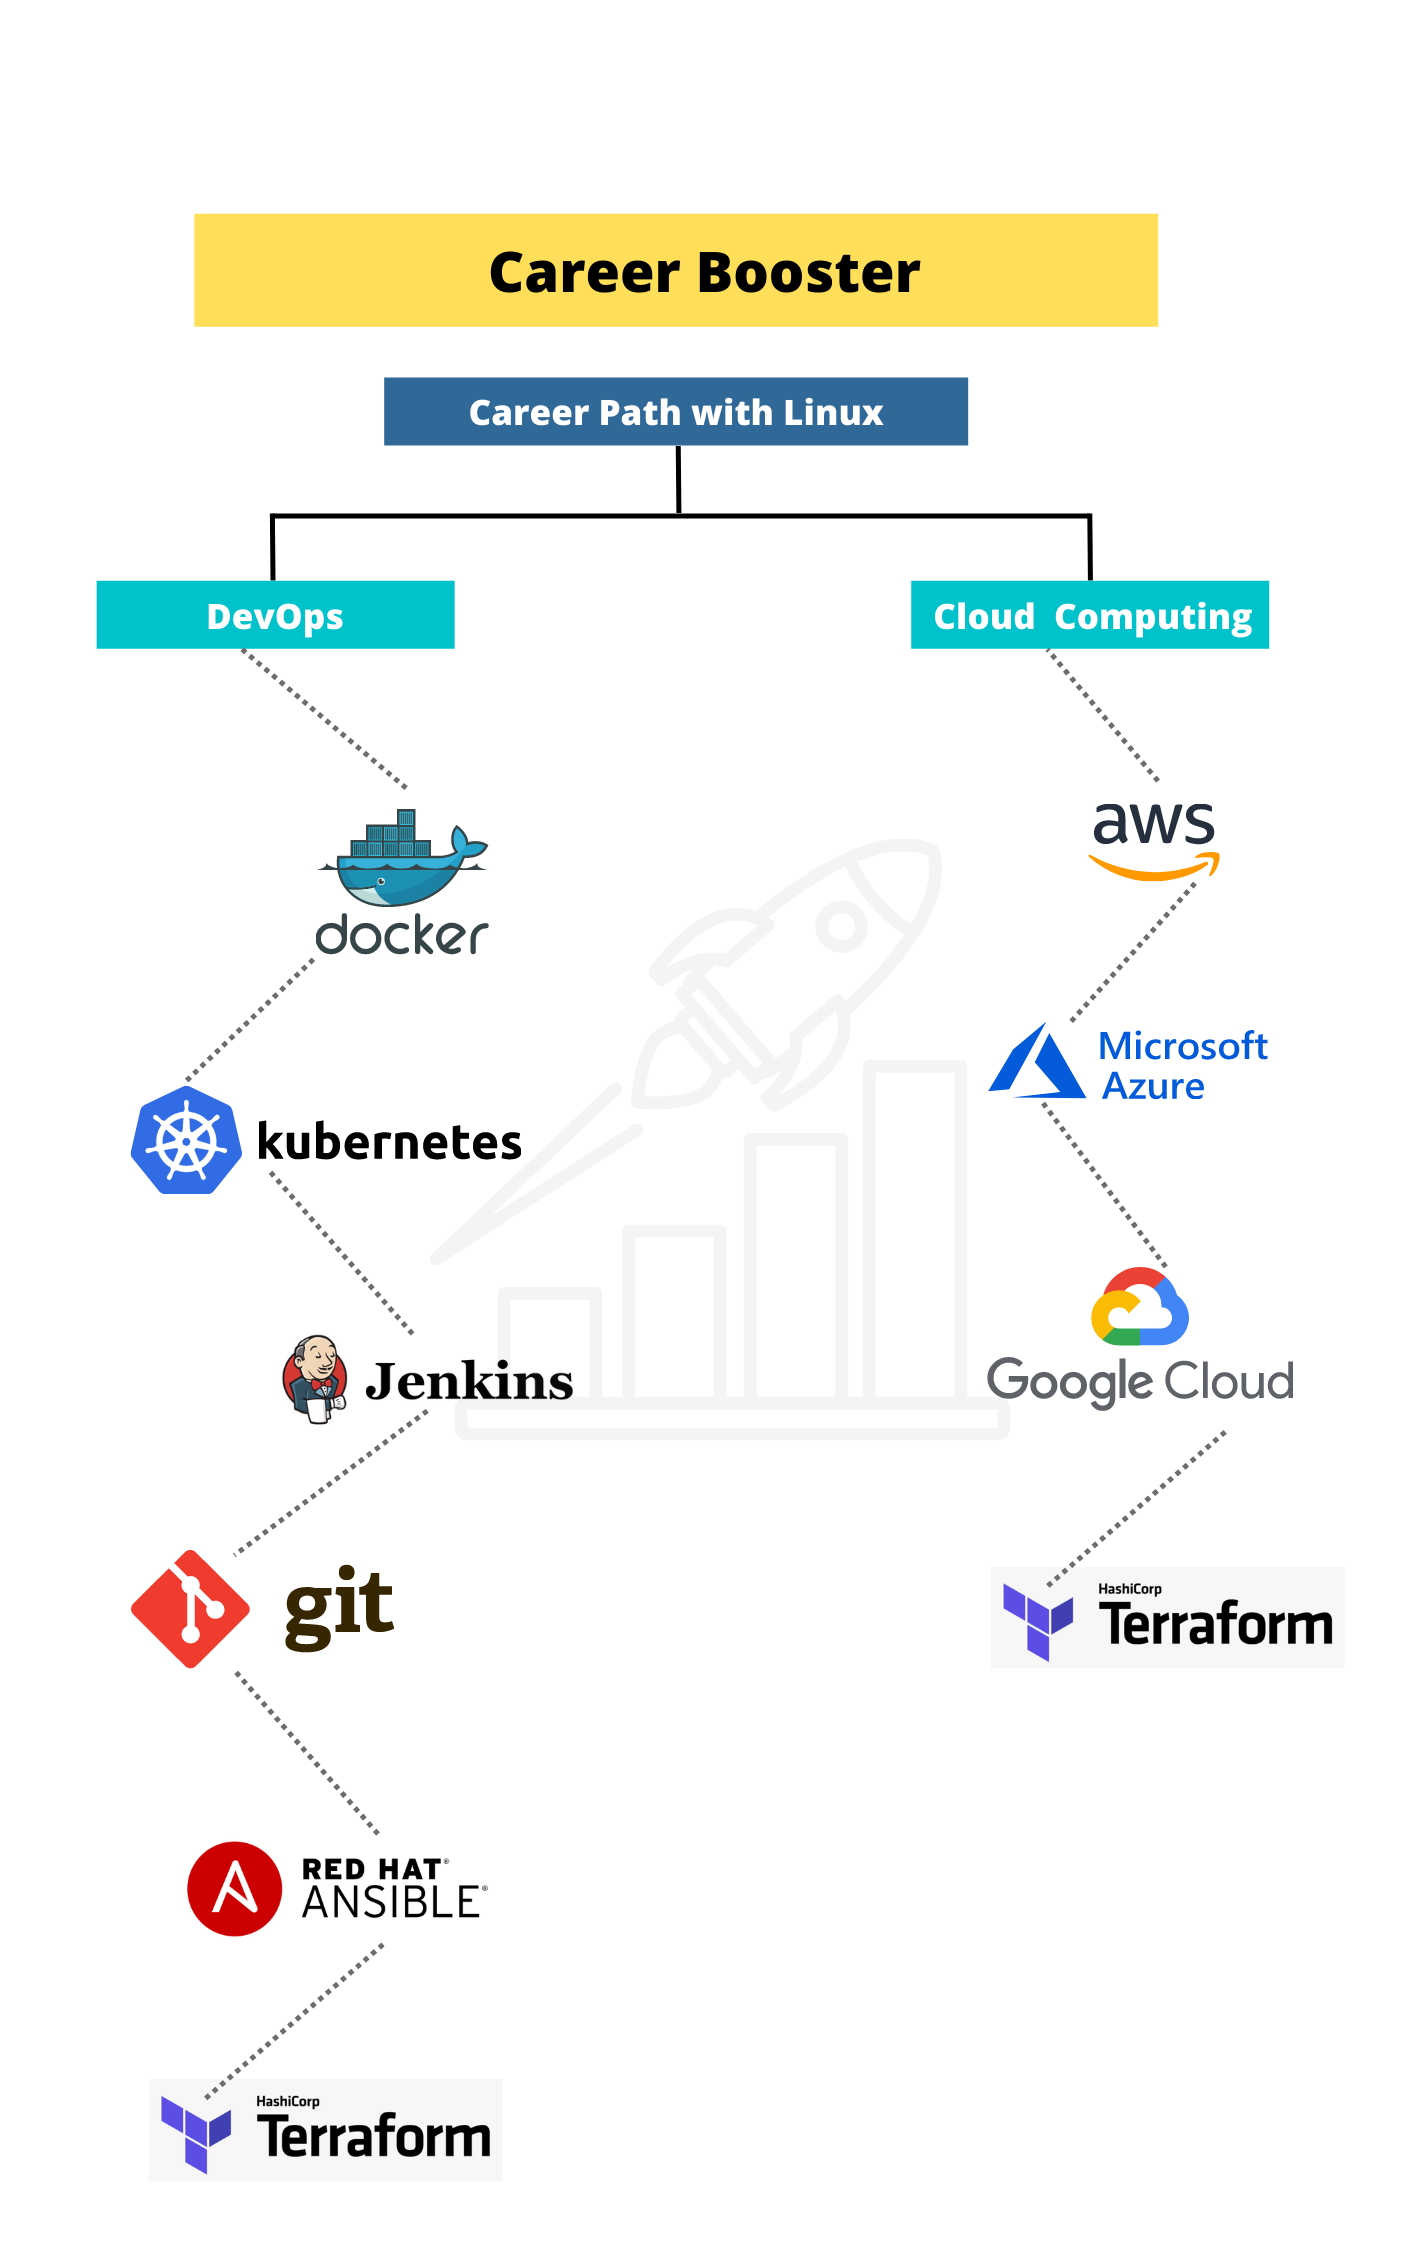
\includegraphics[scale=.35]{content/chapter1/images/career.png}
\end{figure}

\newpage
\paragraph{Linux Job Titles}
\bigskip
\bigskip
When you're looking for Linux jobs you can earn different job titles. Here are a few to watch out for:
\begin{itemize}
	\item Linux Administrator
	\item Linux System Administrator
	\item Linux System Engineer
	\item Linux Engineer
	\item Operations Engineer
	\item SRE (Site Reliability Engineer)
	\item DevOps Engineer
	\item Platform Engineer
	\item Sysadmin
	\item Release Engineer
	\item Build Engineer
	\item Security Administrator
\end{itemize}

There will be even more variations to the job titles when you add prefixes such as "Junior", "Senior" or "Associate" to the mix.

\end{flushleft}


\newpage

\chapterimage{index2.png}
\chapter{Introduction to Java}
\section{Getting started with Java}

\setlength{\columnsep}{3pt}
\begin{flushleft}
	\bigskip
	\bigskip
	\begin{tcolorbox}[breakable,notitle,boxrule=1pt,colback=black,colframe=black]
	\color{white}
	\bigskip
	In this section, you are going to learn:
	\begin{enumerate}
		\item \textbf{What is Java?}
		\item \textbf{Uses of Java}
		\item \textbf{Problem with C and C++}
		\item \textbf{Advantages of Java over C++}
		\item \textbf{How does program execution works?}
		\item \textbf{The way Java works}
		\item \textbf{Compiler V/S JVM}
		\item \textbf{JVM components}
		\item \textbf{History of Java}
	\end{enumerate}	
	\end{tcolorbox}

	
	\bigskip
	\bigskip
	
	\begin{multicols}{2}
		\vspace*{\fill}
		\vspace*{\fill}
		\vspace*{\fill}
		\vspace*{\fill}
		\vspace*{\fill}
		\vspace*{\fill}
		\vspace*{\fill}
		\vspace*{\fill}
		\vspace*{\fill}
		
	\end{multicols}	
	
\end{flushleft}

\newpage






\subsection{What is Java?}

\begin{flushleft}

	\begin{itemize}
		\item Java is a popular \textbf{high-level programming language} that is \textbf{platform-independent}, \textbf{object-oriented} and \textbf{open source}.
		\item Let’s understand each bold words in detail:
		\begin{itemize}
			\item \textbf{High level programming langauge}: Language that are in english and can be understood by humans.
			
			\newimage{0.4}{content/chapter0/images/img1.png}
			
			\newpage
			
			\item \textbf{Platform-independent}: Java code can run on any platform (i.e OS) using Java Virtual Machine (JVM). 
			
			\newimage{0.4}{content/chapter0/images/img2.jpg}
						
			\item \textbf{Object-Oriented}: Java is built around objects.
			
			\newimage{0.4}{content/chapter0/images/img3.png}
			
			\item \textbf{Open source}: Java source code is available for anyone to view and modify.
			
			\newimage{0.1}{content/chapter0/images/img4.png}
			
		\end{itemize}
	\end{itemize}
		
\end{flushleft}

\newpage


\subsection{Uses of Java}
\begin{flushleft}
	
	\begin{itemize}
		\item \textbf{Enterprise-level applications} - Eg: SAP, IBM websphere, Salesforce, Oracle E-Business suite
		\newimage{0.3}{content/chapter0/images/1.png}
		\bigskip	
		
		\item \textbf{Web applications} - Eg: LinkedIn, Netflix, Twitter, Amazon, Airbnb
		\newimage{0.3}{content/chapter0/images/2.png}
		
		\item \textbf{Mobile applications} - Eg: Instagram, WhatsApp, Google Maps, Uber
		\newimage{0.3}{content/chapter0/images/3.png}
		\bigskip	
		
		\item \textbf{Games} - Eg: Minecraft, RuneScape, Puzzle Pirates		
		\newimage{0.3}{content/chapter0/images/4.png}
		\bigskip	
		
		\item \textbf{Financial Applications} - Eg: Quicken, Bloomberg Terminal		
		\newimage{0.3}{content/chapter0/images/5.png}
		\bigskip	
		
		\item \textbf{Scientific Applications} - Eg: BioJava, ImageJ		
		\newimage{0.3}{content/chapter0/images/6.png}
		
	\end{itemize}
	
\end{flushleft}

\newpage
\subsection{Problem with C and C++}

\begin{flushleft}
	
	\begin{itemize}
		\item \textbf{Original idea for Java was not the Internet!}
		\item Java was created to be \textbf{platform-independent language} that can be embedded in electronic devices, eg: \textbf{microwave ovens and remote controls}. 
		\item Problem with C and C++  is they are \textbf{compiled for a specific target}. 
		\item James Gosling (founder of Java) began work on a portable, platform-independent language that could be used to produce code that would run on any CPUs.
		\item This led to the creation of Java.
	\end{itemize}

\end{flushleft}



\subsection{Advantages of Java over C++}
\begin{flushleft}
	
	\begin{itemize}
		\item \textbf{Security}: No danger of reading bogus data when accidentally going over the size of an array.
		
		\item \textbf{Automatic memory management}: Garbage collector allocate and deallocate memory for objects. 
		
		\item \textbf{Simplicity}: 
		\begin{itemize}
			\item No pointers, unions, templates, structures, multiple inheritance. 
		\end{itemize}
		
		\item \textbf{Support multithreaded application}
		
		\item \textbf{Portability}: Support WORA (Write it once, run it anywhere), using Java virtual machine (JVM).
		
	\end{itemize}

\end{flushleft}

\newpage
\subsection{How does program execution works?}
\begin{flushleft}
	
	\begin{itemize}
		\item \textbf{Compiler: }
		\begin{itemize}
			\item A compiler is a \textbf{software program that converts source code written in a high-level programming language into machine code}, which can be executed by a computer. 
			\item The compiler performs:
			\begin{itemize}
				\item Syntax analysis
				\item Semantic analysis
				\item Bytecode generation
			\end{itemize}
		\end{itemize}
		
		
		\item \textbf{Interpreter:}
		\begin{itemize}
			\item An interpreter is a program that reads and executes code \textbf{line-by-line}, without the need to compile the entire program beforehand. 
			\item Interpreters run code in a virtual environment, where each line of code is executed as soon as it is read. 
		\end{itemize}
		
		\newimage{0.4}{content/chapter0/images/new03.png}
		
		\item \textbf{Java Virtual Machine (JVM):}
		\begin{itemize}
			\item The JVM is a virtual machine that is responsible for executing Java bytecode. 
			\item The JVM is an example of an interpreter, as it reads Java bytecode and executes it line-by-line. 
			\item The JVM performs:
			\begin{itemize}
				\item Memory management
				\item Security
				\item Garbage collection
			\end{itemize}  
		\end{itemize}
		
	\end{itemize}
	
\end{flushleft}

\newpage
\subsection{The way Java works}
\begin{flushleft}
	
	\textbf{So, what exactly happens to developer-written Java code until the actual execution?}
	
	\newimage{0.35}{content/chapter0/images/new01.png}
	\newimage{0.35}{content/chapter0/images/new02.png}
\end{flushleft}

\newpage
\subsection{Compiler V/S JVM}
\begin{flushleft}
	
	\quest{Compiler and JVM battle over the question, “Who’s more important?”}{
		Go through below discussion to find the answer:\\ \\
		\textbf {JVM:} I am Java. I’m the guy who actually makes a program run. The compiler just gives you a file in bytecode after checking it’s syntax. I'm the one who run it.
		\\ \\
		\textbf{Compiler:} Excuse me? Without me, you would have to translate everything from source code and be very very slow!
		\\ \\	
		\textbf{JVM:} Your work is not important. A programmer could just write bytecode by hand. You might be out of a job soon, buddy.
		\\ \\
		\textbf{Compiler:} That’s arrogant. A programmer writing bytecode by hand is next to possible, some scholars might write, not everyone!
		\\ \\
		\textbf{JVM:} But you still didn’t answer my question, what you actually do?
		\\ \\
		\textbf{Compiler:} Remember that Java is a strongly-typed language, I can’t allow variables to hold data of the wrong type. This is a security feature, implement by ME!
		\\ \\
		\textbf{JVM:} Your type checking is not very strict! Sometimes people put the wrong type of data in an array of different type.
		\\ \\
		\textbf{Compiler:} Yes, that can emerge at runtime that only you can catch to allow dynamic binding. But my job is to stop anything that would never succeed at runtime. 
	}
	
	\newpage
	
	\anscontinue{
	
	\textbf{JVM:} OK. Sure. But what about security? Look at all the security stuff I do! You just perform silly syntax checking.
	\\ \\
	\textbf{Compiler:} Listen, I'm the first line of defense. I also prevents access violations, such as code trying to invoke a private method. I stop people from touching code they’re not meant to see.
	\\ \\
	\textbf{JVM:} Whatever. I have to do that same stuff too!
		
	}
\end{flushleft}

\subsection{JVM components}
\begin{flushleft}
	
	\newimage{0.5}{content/chapter0/images/new05.png}
	\begin{itemize}
		\item \textbf{Class Loader:} Responsible for loading the class files into the memory of the JVM.
		\item \textbf{Execution Engine:} Responsible for executing the bytecode that is loaded into the memory. It includes:
		\begin{itemize}
			\item \textbf{Interpreter:} Reads and executes the bytecode one instruction at a time. 
			\item \textbf{JIT compiler:} Compiles the bytecode into machine code for fast execution.
		\end{itemize}
		
		\item \textbf{Garbage Collector:} It periodically frees up the memory that is not used by the Java application.
		
		\item \textbf{Runtime Data Area:} It is memory space allocated by the JVM for the execution of the Java application. It includes:
		\begin{itemize}
			\item Method area
			\item Heap
			\item Stack
			\item PC registers
		\end{itemize}
		\item \textbf{Native Method Interface (JNI):} Allows Java code to call code written in other programming languages like C and C++. The JNI allows Java applications to interact with OS and hardware.
		
	\end{itemize}
	
	
\end{flushleft}

\newpage
\subsection{History of Java}
\setlength{\columnsep}{20pt}
\begin{flushleft}

	\item \quest{What year Java was invented?}{1995}

	\bigskip
	\quest{What company invented Java?}{Sun Microsystems \\ \\
		\boximage{0.3}{content/chapter0/images/sun.png}
	}

	\bigskip
	\quest{Who is founder of Java?} {
	James Gosling  \\ \\
	\boximage{0.3}{content/chapter0/images/james.jpg}
	}
  
  	\bigskip
  	\quest{What is Java mascot?}{
  	A cartoon character named Duke \\ \\
  	\boximage{0.3}{content/chapter0/images/mascot.png}
  	}
  
  	\bigskip
  	\quest{What is the original name of Java ?}{
  	"Oak" after the oak tree that was outside Gosling's office. 
  	}

	\bigskip
	\quest{What was the reason for changing original name?}{
	"Oak" was already trademarked	
	}
	
	\bigskip
	\quest{What is the inspiration behind Java's name?}{
	Java language is named after coffee grown on the Indonesian island
	}
	
	\bigskip
	\quest{What is original Java logo?}{
		Original logo: \\ \\
	\boximage{0.3}{content/chapter0/images/jlogo.png}
	}

	\bigskip
	\quest{Who has the current ownership of Java?}{Oracle acquired Java in 2009}
	
	\newpage
	
	\quest{What are the Java versions?}{
		Below are the Java version details:
		
		\tableinsidebox{
		\hline
		Version &  Year \\
		\hline
		JDK Alpha and Beta & 1995  \\
		\hline
		JDK 1.0 & Jan, 1996 \\
		\hline
		JDK 1.1 & Feb, 1997 \\
		\hline
		J2SE 1.2 or \textbf{Java2} (codename: Playground) & Dec, 1998 \\
		\hline
		J2SE 1.3 or \textbf{Java2} (codename: Kestrel) &  May, 2000 \\
		\hline
		J2SE 1.4 or \textbf{Java2} (codename: Merlin) & Feb, 2002 \\
		\hline
		J2SE 1. 5 or \textbf{Java5} (codename: Tiger) & Sep, 2004 \\
		\hline
		Java SE 1.6 or \textbf{Java6} (codename: Mustang) &  Dec, 2006 \\
		\hline
		Java SE 1.7 or \textbf{Java7} (codename: Dolphin) & July, 2011 \\
		\hline
		Java SE 1.8 or \textbf{Java8} (codename: Spider) & (18th March, 2014) \\
		\hline
		Java SE 1.9 or \textbf{Java9} & September, 2017 \\
		\hline
		\textbf{Java 10} & March, 2018 \\
		\hline
		\textbf{Java SE 11} & September 2018 \\
		\hline
		\textbf{Java SE 12} & March 2019 \\
		\hline
		\textbf{Java SE 13} & September 2019 \\
		\hline
		\textbf{Java SE 14} & March 2020 \\
		\hline
		\textbf{Java SE 15} & September 2020 \\
		\hline
		\textbf{Java SE 16} & March 2021 \\
		\hline
		\textbf{Java SE 17} & September 2021 \\
		\hline
		}
		
	}

	\newpage
	\quest{Why is Java 2 consider very significant in history of Java?}{		
		Starting \textbf{Java 2}, it is composed of three parts:
		\begin{itemize}
			\item \textbf{J2SE (Java 2 Platform, Standard Edition) or JSE}, a computing platform for the development and deployment of portable code for \textbf{desktop and server environments}.
			\item \textbf{J2EE (Java 2 Platform, Enterprise Edition) or JEE}, extending Java SE with enterprise features such as \textbf{distributed computing and web services}.
			\item \textbf{J2ME (Java 2 Platform, Micro Edition) or JME}, a computing platform for \textbf{embedded and mobile devices}.
		\end{itemize}
		Other major highlights of this release:
		\begin{itemize}
			\item \textbf{JIT compiler} became part of JVM (means turning code into executable code became a faster operation).
			\item \textbf{Swing graphical API} was introduced as alternative to AWT.
			\item Java collections framework (for working with sets of data) was introduced.
		\end{itemize}
	}

	\quest{I see Java 2 and Java 5.0, but was there a Java 3 and 4? And why is it Java 5.0 but not Java 2.0?}{
		The joys of marketing... 
		\begin{itemize}
			\item When the version of Java shifted from 1.1 to 1.2, the changes to Java were so many that the marketers decided a whole new “name”, so they started calling it Java 2, even though the actual version of Java was 1.2.
			\item But versions 1.3 and 1.4 were still considered Java 2.
			\item There never was a Java 3 or 4. 
			\item Beginning with Java version 1.5, the marketers decided a new name was needed. 
			\item The next number in the name sequence would be “3”, but calling Java 1.5 Java 3 seemed more confusing, so they decided to name it Java 5.0 to match the “5” in version “1.5”. 	
		\end{itemize}
	}

\end{flushleft}



\section{Installing Java and IDE}
\setlength{\columnsep}{3pt}
\begin{flushleft}
	\bigskip
	\bigskip
	\begin{tcolorbox}[breakable,notitle,boxrule=1pt,colback=black,colframe=black]
		\color{white}
		\bigskip
		In this section, you are going to learn:
		\begin{enumerate}
			\item \textbf{Java installation}
			\item \textbf{IDE installation}
			\item \textbf{Our first Java program}
			\item \textbf{Using JShell}
		\end{enumerate}	
	\end{tcolorbox}

\end{flushleft}
\newpage

\subsection{Java installation}
\setlength{\columnsep}{5pt}
\begin{flushleft}

	On Ubuntu, open terminal \& follow below steps:
	\begin{itemize}
		\item First check if Java is already installed:
		\commandblock{
			\$ \textbf{java -version} \\
			Command 'java' not found
		}
		\item Install the Java Development Kit (JDK) with the following command:
		\commandblock{
			\$ \textbf{sudo apt install default-jdk -y} \\
			Setting up default-jdk-headless (2:1.11-72build2) ...
		}
		
		\item Install JRE with the following command:
		\bigskip
		\commandblock{
			\$ \textbf{sudo apt install default-jre -y} \\
			Setting up default-jre (2:1.11-72build2) ...
		}
		
		\item Optionally, you can install source code of Java:
		\bigskip
		\commandblock{
		\$ sudo apt-get install openjdk-11-source -y
		}
		\item Configure JAVA\_HOME on Ubuntu, for this locate your Java installation on Ubuntu using below command:
		\commandblock{
			\$ update-alternatives --config java \\
			There is only one alternative in link group java (providing /usr/bin/java): 
			\textbf{/usr/lib/jvm/java-11-openjdk-amd64/bin/java}
		}
	
		\item Add JAVA\_HOME to the environment:
		\bigskip
		\commandblock{
		\$ sudo vi /etc/environment \\
		JAVA\_HOME="/usr/lib/jvm/java-11-openjdk-amd64/bin/java"	
		}
	
		\item Reload the environment configuration file:
		\bigskip
		\commandblock{
			source /etc/environment
		}
		\item Confirm Java is installed:
		\bigskip
		\commandblock{
			\$ java -version \\
			openjdk version "11.0.20" 2023-07-18
		}
		
	\end{itemize}
	
	On Windows, follow below steps:
	
	\begin{itemize}
		\item Open a command prompt by typing \textbf{cmd} in the search bar and press \textbf{Enter}.
		
		\item Check if Java is installed by running following command:
		\newimage{0.65}{content/chapter1/images/one.png}

		\item Navigate to the https://www.oracle.com/java/technologies/downloads/\#jdk17-windows  \& click the x64 Installer download link:
		\newimage{0.5}{content/chapter1/images/two.png}
		
		Double-click the downloaded file to start the installation.
		\newpage
		\item Configure the Installation Wizard:
		\newimage{0.5}{content/chapter1/images/three.png}
		
		\item Choose the destination folder for the Java installation files or stick to the default path. Click Next to proceed.
		\newimage{0.5}{content/chapter1/images/four.png}
		
		\item Click Close to exit the wizard.
		\newimage{0.5}{content/chapter1/images/five.png}
		
		\item Add Java to system variables. Open the Start menu and search for environment variables. Select the Edit the system environment variables result.
		\newpage		
		\newimage{0.5}{content/chapter1/images/siz.png}
		
		\item In the System Properties window, under the Advanced tab, click Environment Variables…

		\newimage{0.35}{content/chapter1/images/seven.png}
		
		\item Under the System variables category, select the Path variable and click Edit:
		
		\newimage{0.4}{content/chapter1/images/eight.png}
		\newpage
		\item Click the New button and enter the path to the Java bin directory:
		
		\newimage{0.5}{content/chapter1/images/nine.png}
		
		\item Add \textbf{\textbf{JAVA\_HOME}} variable. In the Environment Variables window, under the System variables category, click the New… button to create a new variable.

		\newimage{0.5}{content/chapter1/images/ten.png}
		
		\item Name the variable as \textbf{JAVA\_HOME}. 
		
		\item In the variable value field, paste the path to your Java jdk directory and click OK.
		\newpage
		\newimage{0.5}{content/chapter1/images/11.png}
		
		\item Confirm the changes by clicking OK in the Environment Variables and System properties windows.
		
		\item Test the Java Installation:
		
		\newimage{0.6}{content/chapter1/images/12.png}
		
		
	\end{itemize}
	
\end{flushleft}

\subsection{IDE installation}
\setlength{\columnsep}{5pt}
\begin{flushleft}

	Download and install VScode using this link on Microsoft Windows: https://code.visualstudio.com/download

\end{flushleft}


\subsection{Our first Java program}
\setlength{\columnsep}{5pt}

\begin{flushleft}

\begin{itemize}
	\item Code structure in Java:
	\newimage{0.35}{content/chapter0/images/new06.png}
	
	\quest{What goes in a source file?}{
		\begin{itemize}
			\item A source code file with the \textbf{“.java”} extension holds one class definition. 
			\item The source file name should be \textbf{"classname.java"}.
			\item The class represents a piece of your program. 
			\item The class must go within a pair of curly braces.
			\item Eg: Below code name will be Dog.java and class name will be Dog - \\
			\boximage{0.3}{content/chapter0/images/new07.png}
		\end{itemize}
	}
	\bigskip
	\quest{What goes in a class?}{
		\begin{itemize}
			\item A class has one or more methods. 
			\item Your methods must be declared inside a class.
			\item Eg: The class Dog contains a method called bark()
			\\
			\boximage{0.3}{content/chapter0/images/new08.png}
		\end{itemize}	
	}
	\bigskip
	\quest{What goes in a method?}{
		\begin{itemize}
			\item Method code is basically a set of statements.
			\item Method kind of like a function or procedure.
			\item When the JVM starts running, it looks for the method inside the class that looks exactly like:
			\codeblock{
				public static void main (String[] args) \{ \\
				\s 	// your code goes here \\
				\}
			}
			\item JVM runs everything inside \{ \} of your main method. 
			\item Every Java application has to have at least one class, and at least one main method (not one main per class; just one main per application).
		\end{itemize}
	}

	\textbf{Overall, a basic Java program would look something like below:}
	\newimage{0.35}{content/chapter0/images/new09.png}
	
	\bigskip
	\textbf{Running your Java Code:}
	\newimage{0.3}{content/chapter0/images/new10.png}
	
\end{itemize}

				
\end{flushleft}


\subsection{Executing our first Java program}
\setlength{\columnsep}{5pt}
\begin{flushleft}

		\begin{itemize}
			\item Using simple text editor:
			\bigskip
			\codeblockfull{MyFirstApp.java}{
				public class MyFirstApp \{ \\
				\s	public static void main(String[] args) \{ \\
				\s \s		System.out.println("I Rule!"); \\
				\s \s		System.out.println("The World"); \\
				\s	\} \\
				\}	
		
			}
			\bigskip
			\commandblock{
				javac MyFirstApp.java \\
				java MyFirstApp 
			}
			\bigskip
			\outputblock{
				I Rule! \\
				The World
			}
		
			\newpage
			\item Using Eclipse:		
			\begin{enumerate}
				\item Create New Project:
				\\
				\textbf{File -> New -> Java Project -> Add “Starter”} as project name
				
				\newimage{0.35}{content/chapter0/images/new11.png}
				
				\item This will create directory structure as shown below:
				
				\newimage{0.8}{content/chapter0/images/new12.png}
				
				\newpage
				\item Right click the src -> Select “Package” -> Add “Start1” as package name as shown below:
				
				
				\newimage{0.35}{content/chapter0/images/new13.png}
				
				\item Right click the “Start1” -> Select New -> Class -> Add “MyFirstClass” as classname as shown below:
				
				\newimage{0.4}{content/chapter0/images/new14.png}
				
				\newpage
				\item This will create a class with below structure:
				\bigskip
				\codeblock{
					package Start1; \\
					public class MyFirstClass \{ \\
					\s	public static void main(String[] args) \{ \\
					\s	\s	// TODO Auto-generated method stub \\
					\s \s	System.out.println("Welcome Back!"); \\
					\s	\} \\
					\}
				}
			
				\item Execute the code by pressing the run button:
				
				\newimage{0.65}{content/chapter0/images/new15.png}
				
			\end{enumerate}
			
			
		\end{itemize}
		
\end{flushleft}

\newpage

\subsection{Using JShell}
\setlength{\columnsep}{5pt}
\begin{flushleft}

	\begin{itemize}
		\item Introduced in Java9, JShell is a Read-Eval-Print Loop (REPL)
		\item It evaluates declarations, statements, and expressions as they are entered, and then it immediately shows the results.
		\item To use jshell, type “jshell” command in command prompt:
		\bigskip
		\commandblock{
			\$ jshell  \\
			jshell> int i=42; \\
			i ==> 42 \\
			\\
			jshell> float j=3.4f; \\
			j ==> 3.4 \\
			\\
			jshell> i+j \\
			\$3 ==> 45.4 \\
			\\
			jshell> String text = "Welcome To World of Java"; \\	
			text ==> "Welcome To World of Java" 
		}
		
		\newpage
		\item To display all variables declared:
		\bigskip
		\commandblock{
			jshell> /vars \\
			|    int i = 42 \\
			|    float j = 3.4 \\
			|    float \$3 = 45.4 \\
			|    String text = "Welcome To World of Java" \\
			|    String \$5 = "WELCOME TO WORLD OF JAVA"
		}
	
		\item To save all valid statements of Jshell to a file:
		
		\commandblock{
			jshell> /save filename.java \\
			\\
			jshell> /exit \\
			|  Goodbye
		}
		
		\item Content of filename.java:
		\codeblockfull{filename.java}{
			int i=42; \\
			float j=3.4f; \\
			i+j \\
			String text = "Welcome To World of Java"; \\
			text.toUpperCase()
		}
		
		\item You can open the file back in the jshell using open command:
			\commandblock{
				jshell> /open filename.java \\
				 \\
				jshell> i \\
				i ==> 42
			}
		
	\end{itemize}

\end{flushleft}




%--------------------------------------------------------------------------
%	CHAPTER 2
%-------------------------------------------------------------------------

\chapterimage{index3.png} % Table of contents heading image
\chapter{Java Language Fundamentals}
%-----------------------
\section{Identifiers, variables and more}
\setlength{\columnsep}{3pt}
\begin{flushleft}
	\bigskip
	\bigskip
	\begin{tcolorbox}[breakable,notitle,boxrule=1pt,colback=black,colframe=black]
		\color{white}
		\bigskip
		In this section, you are going to learn:
		\begin{enumerate}
			\item \textbf{Java identifiers}
			\item \textbf{Java grammar}
			\item \textbf{Java variable}
			\item \textbf{Literals}
			\item \textbf{Java reserved words or keywords}
			\item \textbf{Java comments}
			\item \textbf{How objects can change your life?}
		\end{enumerate}	

	\end{tcolorbox}
		
\end{flushleft}

\newpage






\subsection{Java identifiers}

\begin{flushleft}
	
	A Java identifier is a name of a variable, function, class, module or other object.
	\newline
	Eg:
	\begin{tcolorbox}[breakable,notitle,boxrule=-0pt,colback=code,colframe=code]
		\color{black}
		\fontdimen2\font=8pt
		package \textbf{Starter}; \newline
		\newline
		public class \textbf{Test} \{ \newline
		\hphantom{} \hphantom{}	public static void main(\textbf{String}[] \textbf{args}) \{ \newline
		\hphantom{} \hphantom{} \hphantom{} \hphantom{}	int \textbf{x}=999; \newline
		\hphantom{} \hphantom{} \hphantom{} \hphantom{}	System.out.println(x); \newline
		\hphantom{} \hphantom{}	\} \newline
		\}
		\fontdimen2\font=4pt
	\end{tcolorbox}
	
	\bigskip
	In above code, there are total 6 identifiers:
	\begin{itemize}
		\item Starter - name of package
		\item Test - name of class
		\item main - name of function
		\item String - name of class 
		\item args - name of object
		\item x - name of integer variable
	\end{itemize}
	
	\textbf{Rules of identifiers:}
	\begin{itemize}
		\item Names can contain A-Z, a-z, 0-9, \_, and \$ signs.
		\item Names cannot begin with number.
		\item Names are case sensitive ("myVar" and "myvar" are different variables).
		\item Reserved words (like Java keywords, such as int or boolean) cannot be used as names.
		\item Names can be of any length, but it's not recommended to have big names.
		\item Developers should declare identifiers using the \textbf{Camel case} writing style (e.g., StringBuilder, isAdult)
	\end{itemize}
	
	\bigskip
	\begin{figure}[h!]
		\centering
		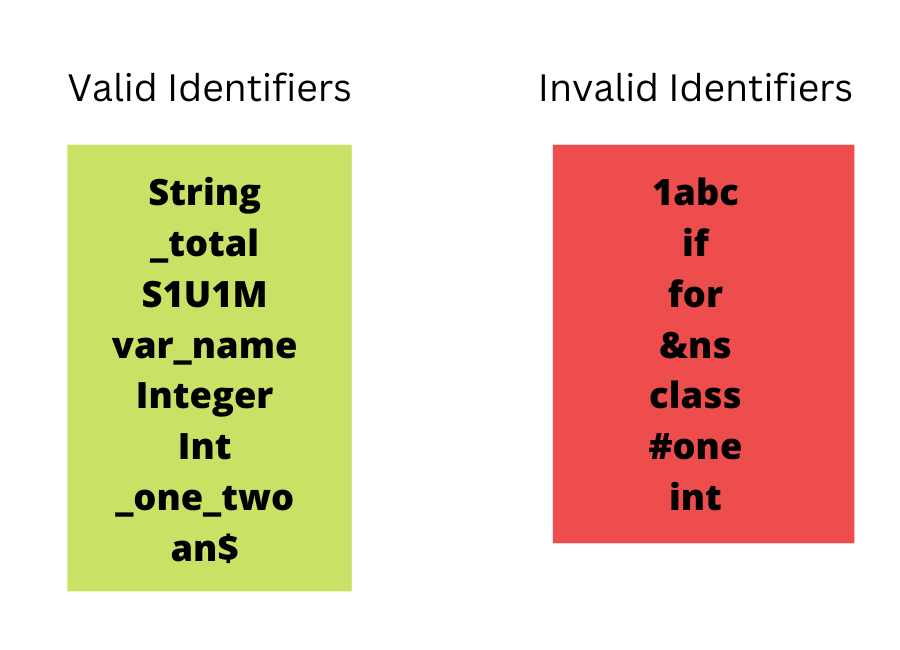
\includegraphics[scale=.45]{content/chapter2/images/java.png}
	\end{figure}
	
	
\end{flushleft}



\subsection{Java grammar}

\begin{flushleft}
	
	\begin{itemize}
		
		\item Java is \textbf{case sensitive}.
		\item \textbf{Block delimiters}: Except for import, package, interface (or @interface), enum and class declarations, everything else in a Java source file must be declared between curly brackets ({}).
		\item Code lines are ended in Java by the \textbf{semicolon (;) symbol}

	\end{itemize}	
	
	
\end{flushleft}

\subsection{Java variable}

\begin{flushleft}
	\begin{itemize}
		\item The variable is the basic unit of storage in a Java program.
		\bigskip
		\syntaxblock{
			type identifier = value; \\
			or  \\
			type identifier = value, identifier = value, identifier = value ... ;
		}
		Here, 
		\begin{itemize}
			\item type = datatype or name of class or interface
			\item identifier = name of variable
		\end{itemize}
		
		\bigskip
		To declare more than one variable of the specified type, use a comma-separated list.
		\bigskip
		\codeblockfull{New.java}{
			class New \{ \\
			\s	public static void main(String[] args) \{ \\
			\s \s	int a, b, c; \\
			\s \s	int d = 3, e, f = 5; \\
			\s \s	byte z = 22; \\
			\s \s	double pi = 3.14159; \\
			\s \s	char x = 'x'; \\
			\s	\} \\
			\} 
		}
			
	\end{itemize}	
		
\end{flushleft}
\newpage

\subsection{Literals}

\begin{flushleft}


	\begin{itemize}
		\item A constant value which can be assigned to the variable is called \textbf{literal}
		\item Eg:
		\begin{figure}[h!]
			\centering
			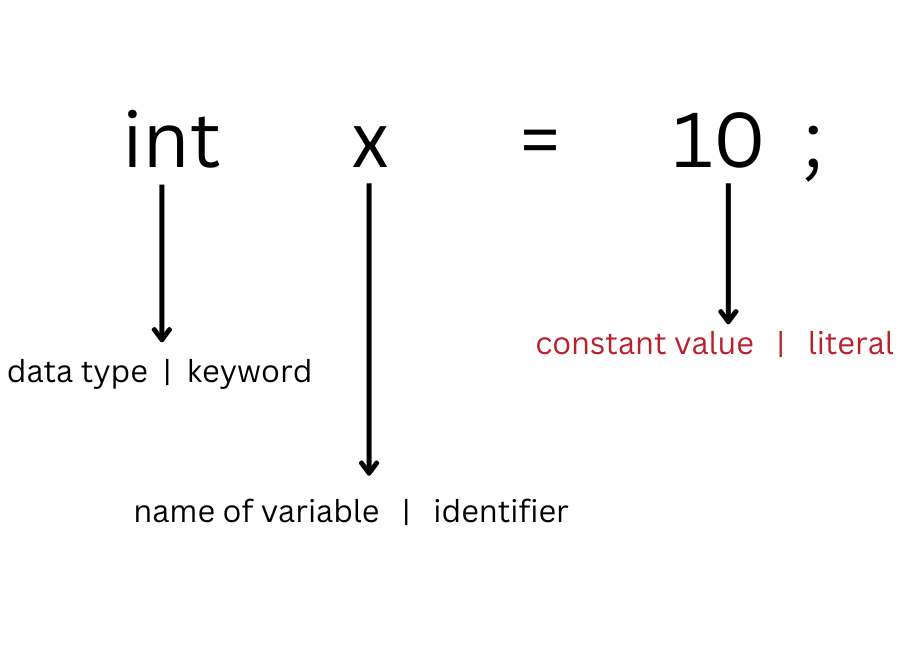
\includegraphics[scale=.4]{content/chapter2/images/literal.png}
		\end{figure}		
		
	\end{itemize}


	
\end{flushleft}




\subsection{Java reserved words or keywords}

\begin{flushleft}
	
	\begin{itemize}
		
		\item Words having \textbf{predefined meaning}
		\item Java 17 has a total of 60 reserved words.
		
		\begin{figure}[h!]
			\centering
			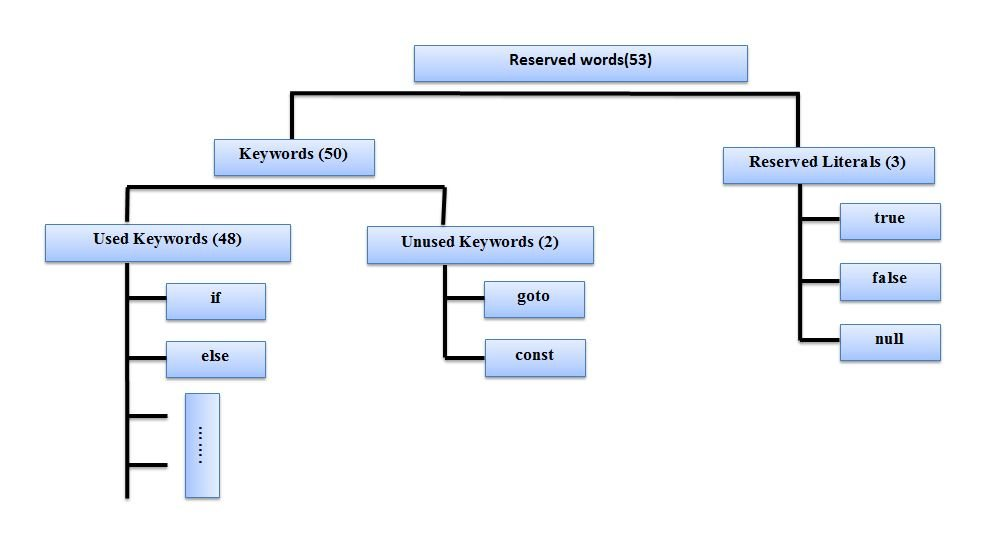
\includegraphics[scale=.45]{content/chapter2/images/reserve1.jpg}
		\end{figure}		
		
		\begin{figure}[h!]
			\centering
			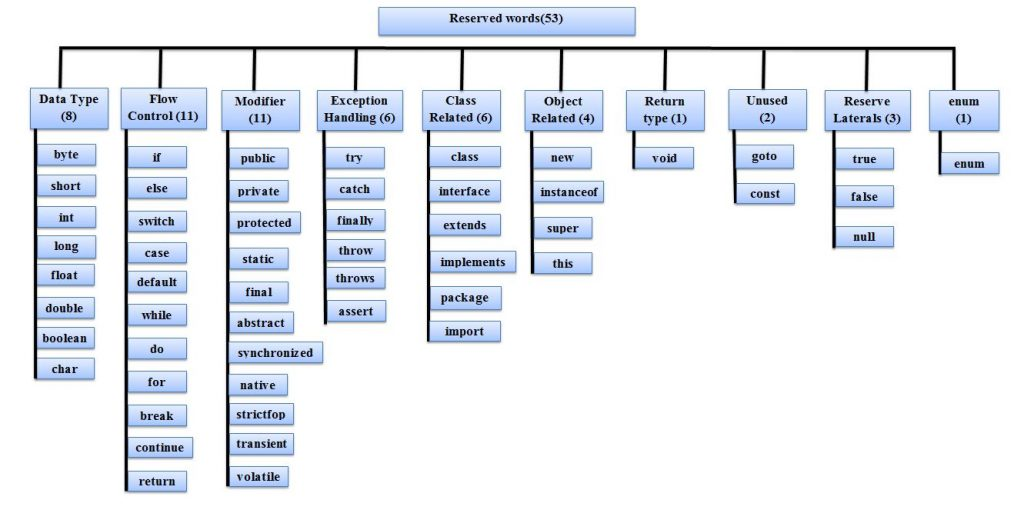
\includegraphics[scale=.6]{content/chapter2/images/reserve2.jpg}
		\end{figure}		
	
			
	\end{itemize}	

	\noteblock{
		\textbf{const} and \textbf{goto} are not used anymore!		
	}
	
	
		
	
\end{flushleft}
\newpage

\subsection{Java Comments}

\begin{flushleft}
	
	\begin{itemize}
		
		\item Java comments refer to text that are not considered part of the code execution and ignored by the compiler. 
		\item 3 ways to add comments:
		\begin{itemize}
			\item \textbf{//} : Used for single line comments:
			\bigskip
			\codeblock{
				\s // testing
			}
			\item \textbf{/** ... */}: Javadoc comments, special comments that are exported using special tools into the documentation of a project called Javadoc API
			\bigskip
			\codeblock{
				/** \\
				* Returns the sum of two integers. \\
				* @param a the first integer to add \\
				* @param b the second integer to add \\
				* @return the sum of a and b \\
				*/ \\
				public int add(int a, int b) \{ \\
				\s	return a + b; \\
				\}	 
			}
		
			\item \textbf{/* ... */} : used for multiline comments
			\bigskip
			\codeblock{
				/* This is  \\
				a multi line  \\
				statement */ 
			}
		\end{itemize}
	
		
		
		
		
		
		
		
	\end{itemize}	
	
	
\end{flushleft}
\newpage

\subsection{How Objects Can Change Your Life?}

\begin{flushleft}
	\begin{itemize}
		
		\item So far, we put all of our code in the \textbf{main() method}. 
		\item \textbf{That’s not exactly object-oriented}. 
		\item Leave the procedural world behind, get the out of main(), and start making some objects of our own. 
		\item We’ll look at what makes object-oriented (OO) development in Java so much fun. 
		\item Let’s understand this with a use-case:  \\
		Creat a Shape Application with below requirement:
		
		\newimage{0.5}{content/chapter0/images/new16.png}
		
		\item For this, Raj followed Procedure-Oriented approach while Ram followed Object-Oriented approach to develop the code.
		
		\newpage
		\tabletwo{
			\hline
			Raj's Procedure-Oriented approach & Ram's Object-Oriented approach  \\
			\hline
			\bigskip \bigskip
			\codeblock{
				rotate(shapeNum) \{ \\
				\s	//code here \\
				\} \\
				playSound(shapeNum) \{ \\
				\s	//code here \\
				\} 
			} & \bigskip 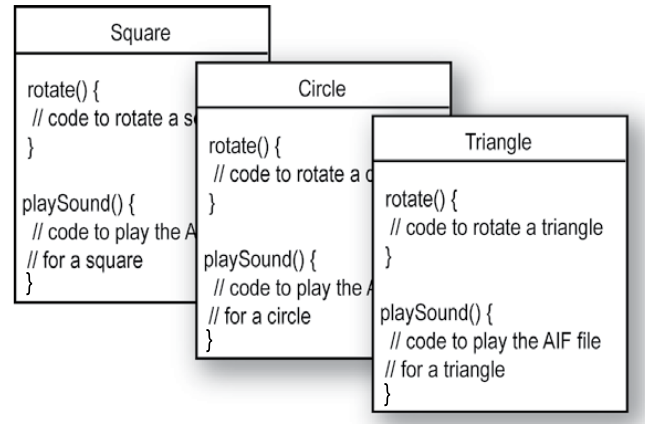
\includegraphics[scale=0.3]{content/chapter0/images/new17.png}  \\
			\hline
		}
		
		\item But wait! There’s been a spec change.
		
		\newimage{0.35}{content/chapter0/images/new18.png}
		
		\item In order to reflect the new requirements, here's what Raj and Ram decided to do:
		
		\newpage
		
		\tabletwo{
			\hline
			Back in Raj's cube  & At Ram's laptop in a cafe  \\
			\hline
			Raj will need to make changes in existing code and perform the testing again:
			\bigskip
			\codeblock{
				\color{red}
				rotate(shapeNum) \{ \\
					//new changes to add amoeba \\
				\} \\
				playsound(shapeNum) \{ \\
					//add change for amoeba \\
				\} 
			} & 
			Ram just need to create one more class called "Amoeba":
			 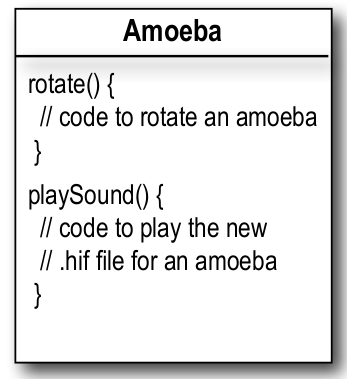
\includegraphics[scale=0.5]{content/chapter0/images/new19.png}  \\
			\hline
		}
	\end{itemize}

	\quest{So what do you like about OO?}{
		\begin{itemize}
			\item Design software as per real world usage.
			\item New changes can be incorported easily.
			\item Not messing around with code already tested, just to add a new feature.
			\item Data \& methods that operate on that data are together in one class.
			\item Code can be re-used in other applications.
		\end{itemize}	
	}
	
	Let’s dig a bit deeper into OOP’s
\end{flushleft}
\newpage

\section{Introductions to OOPs}


\begin{flushleft}
	
	\textbf{O}bject-\textbf{O}riented \textbf{P}rogramming (OOP) is a programming paradigm that revolves around the concept of "objects". 
	\newline
	\newline
	In Java, OOP is implemented through the use of classes and objects.
	\newline \newline
	\textbf{Class \& Object}	
	\begin{itemize}
		\item A class is a blueprint for an \textbf{object}. 
		\item It tells the JVM how to make an object of that particular type.
		\item An Object is real world entity. It is an instance of class.
		
		\newimage{0.5}{content/chapter0/images/new20.png}
		
		\item A class consists of instance \textbf{variable and methods}:
		\begin{itemize}
			\item \textbf{Instance variable:} Represents the object data.
			\item \textbf{Methods:} Things an object can do are called methods.
			\newimage{0.38}{content/chapter0/images/new21.png}
		\end{itemize}
		
		\newpage
		\item Java code for class and object would look something like below:
		
		\newimage{0.5}{content/chapter0/images/new22.png}
		
		\newimage{0.5}{content/chapter0/images/new23.png}	
		
	\end{itemize}
	
\end{flushleft}

\subsection{Pillars of OOPs}


\begin{flushleft}
	
	\begin{itemize}
		\item \textbf{Encapsulation:}
		\begin{itemize}
			\item Technique of bundling data and methods in a class. 
			\item With encapsulation, data cannot be accessed from outside the class. 
			\item This protects the data from accidental modification.
			
			\newimage{0.55}{content/chapter0/images/new25.png}
		\end{itemize}
		
		\item \textbf{Inheritance:}
		\begin{itemize}
			\item Inheritance is one class acquires the properties (methods and fields) of another class.
			\item It allows code reusability and saves time and effort.
			\newimage{0.55}{content/chapter0/images/new26.png}
		\end{itemize}
	
		\newpage
		\item \textbf{Polymorphism: }
		\begin{itemize}
			\item Polymorphism is ability of objects of different classes to be treated as if they belong to a common superclass. 
			\item Polymorphism allows methods to be written that can work with objects of many different classes, as long as they share a common interface. 
			\item This enables code to be more flexible and adaptable to changing requirements.
			\newimage{0.4}{content/chapter0/images/poly.png}
			
		\end{itemize}
	
		\item \textbf{Abstraction:}
		\begin{itemize}
			\item Abstraction hides implementation details.
			\item It shows only the essential features of an object. 
			\newimage{0.55}{content/chapter0/images/new27.png}
		\end{itemize}
		
	
	\end{itemize}
		
	
\end{flushleft}
\newpage




\subsection{main() method}


\begin{flushleft}
	
	\begin{itemize}
		\item \textbf{main()} serves as the entry point for a Java program. 
		\item When a Java program is executed, the JVM starts by looking for the main() method in the class specified in the command line arguments, and then executes the code inside it.
		\bigskip
		\syntaxblock{
			public static void main(String[] args)
		}
		\bigskip
		\item At runtime, JVM always searches for main method with the above prototype:
		\begin{itemize}
			\item \textbf{public:} To call main() from anywhere
			\item \textbf{static:} without existing object also, JVM has to call this method
			\item \textbf{void:} main() method wont return anything to JVM
			\item \textbf{main:} This is the name which is configured inside JVM
			\item \textbf{String[] args:} command line argument
		\end{itemize}
		\bigskip
		\noteblock{
			The main() syntax is very strict and if we perform any change then we will get runtime error from JVM saying “NoSuchMethodError: main”.
		}
		\bigskip
		\item Changes allowed in main():
		\begin{itemize}
			\item Order of modifier can be changed:
			\newline
			Eg: static public void main(String[] args)
			\item The command line argument’s string array can have different syntax:
			\newline
			Eg: public static void main(String args[])
			\item Identifier of the string array can change:
			\newline
			Eg: public static void main(String name[])
			\item String array can be taken as var\_arg parameter
			\newline
			Eg: public static void main(String… args)
			\item main() method can be declared with following modifiers:
			\begin{itemize}
				\item final
				\item synchroised
				\item strictfop
			\end{itemize}
			Eg:
			\codeblockfull{New.java}{
				class New \{ \\
				\s static final synchronized strictfp public void main(String... name)\{ \\
				\s \s System.out.println("Valid main method"); \\
				\s \} \\
				\} 
			}
		\end{itemize}
		\bigskip
		\item There can be multiple main() methods (i.e main() method over-loading is possible!). However JVm will always call String[] argument main method only.
		\bigskip
		\codeblockfull{New.java}{
			class New \{ \\
			\s	public static void main(String[] args)\{ \\
			\s	\s	System.out.println("Starting"); \\
			\s	\}
			\s	public static void main(int[] args)\{ \\
			\s \s		System.out.println("Sample 2"); \\
			\s	\}
			\}
		}
		\bigskip
		\outputblock{
			Starting
		}
		\newpage
		\item \textbf{Inheritance:} While executing child class, if child does not contain main(), then parent class main() will be executed.
		
		\codeblockfull{New.java}{
		class New \{ \\
		\s public static void main(String[] args)\{ \\
		\s \s System.out.println("Starting"); \\
		\s \} \\
		\} \\
		class C extends New \{\}
		}
		\bigskip
		\commandblock{
			\$ javac New.java  <- Creates C.class New.clas New.java  \\ 
			\$ java New \\ 
			Starting \\ 
			\$ java C \\
			Starting
		}
		\bigskip
		\item \textbf{Method hiding}: Child class can override parent class’s main(). This is not method overriding but it is method hiding.
		\newline
		Eg:
		\codeblockfull{New.java}{
			class New \{ \\
			\s	public static void main(String[] args)\{ \\
			\s \s		System.out.println("Starting New"); \\
			\s	\} \\
			\} \\
			class C extends New \{ \\
			\s	public static void main(String[] args)\{ \\
			\s \s		System.out.println("Starting C"); \\
			\s	\} \\
			\} 
		}
		\newpage
		\commandblock{
			\$ javac New.java  <- Creates C.class New.clas New.java  \\ 
			\$ java New \\ 
			Starting New \\ 
			\$ java C \\
			Starting C
		}
	\end{itemize}
	
	
	
	\noteblock{
		\begin{itemize}
			\item Whether class contains main() method or not, and whether main() method is declared according to requirement or not, \textbf{these things are won’t be checked by compiler}.
			\item At runtime, \textbf{JVM is responsible to check these things}.
			\item If JVM unable to find main() method, then will throw runtime exception!
		\end{itemize}
	}
	
\end{flushleft}
\newpage



 
\subsection{Command-line argument}


\begin{flushleft}
	
	\begin{itemize}
			\item Command line arguments are values passed to Java program when it is run from the command line. 
			\item With these command line arguments, JVM creates an array and pass it to main().
			\item Command line arguments can be accessed using the args parameter of the main(). 
			\item Args parameter is an array of String objects.
			\item You can customise behaviour of main() using command-line argument:
			
			\codecontinue{
			public static void main(String[] args) //  ← Here, \textbf{String[] args} contains command line args
			}
		
			\newimage{0.5}{content/chapter2/images/ans.png}
		
			\item Command line argument are always String[]
			
			\codeblockfull{New.java}{
				class New \{ \\
				\s	public static void main(String... args) \{  \\
				\s \s		for(int i = 0; i < args.length; i++) \{ \\
				\s \s			System.out.println(args[i]); \\
				\s \s		\} \\
				\s	\} \\
				\}
			}
		
			\commandblock{
			\$ javac New.java  \\
			\$ java New 1 23 3 \\
			1  \\
			23  \\
			3 \\
			}
			\bigskip
			\item Command line arguments are separated by space. To give one argument with space character, using "" :
			\commandblock{
				\$ java New "Note Book"
			}
			
							
	\end{itemize}
	
	
\end{flushleft}
\newpage



 


\chapterimage{index3.png} % Table of contents heading image
\chapter{Data types in Java}
%-----------------------
\section{Getting started with data type}
\setlength{\columnsep}{3pt}
\begin{flushleft}
	\bigskip
	\bigskip
	\begin{tcolorbox}[breakable,notitle,boxrule=1pt,colback=black,colframe=black]
		\color{white}
		\bigskip
		In this section, you are going to learn:
		\begin{enumerate}
			\item \textbf{Java is strongly typed}
			\item \textbf{Types of data types}
			\item \textbf{Integer data type in detail}
			\item \textbf{Floating-point data type in detail}
			\item \textbf{Character data type in detail}
			\item \textbf{Boolean data type in detail}
		\end{enumerate}	

	\end{tcolorbox}
	
\end{flushleft}

\newpage






\subsection{Java is strongly typed}



\begin{flushleft}
	
	This means:
	\begin{itemize}
		\item Every variable has a type that are strictly defined.
		\item All assignments are checked for type compatibility.
		\item Type mis-match errors must be corrected before compiling the class.
	\end{itemize}
	
	
\end{flushleft}
	





\subsection{Types of data types}
\setlength{\columnsep}{5pt}

\begin{flushleft}
	
	There are two types of data types in Java:
	
	\begin{itemize}
		\item \textbf{Primitive data types}: Includes boolean, char, byte, short, int, long, float and double.
		\item \textbf{Reference data types}: 
		\begin{itemize}
			\item These are not predefined by the language.
			\item They are instead created by the programmer using class definitions. \item Examples of reference data types include:
			\begin{itemize}
				\item Classes
				\item Interfaces
				\item Arrays
				\item Strings
				\item Enumerations
			\end{itemize}
		\end{itemize}
	
	\end{itemize}
	
	We shall see primitive data type in detail in this chapter.
	
\end{flushleft}

\newpage
\section{Integer}

\setlength{\columnsep}{5pt}

\begin{flushleft}
	
	

	\begin{figure}[h!]
		\centering
		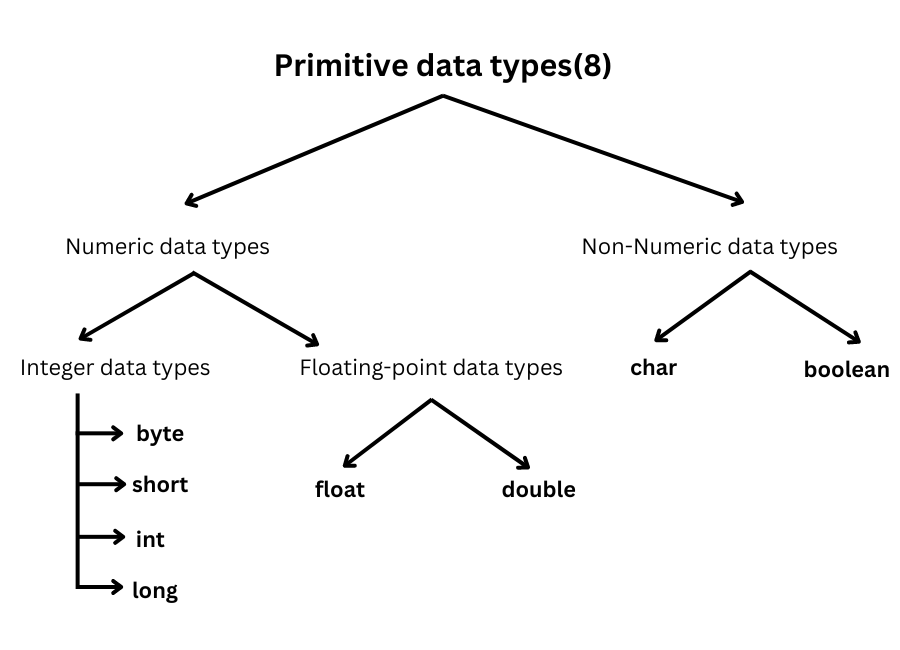
\includegraphics[scale=.6]{content/chapter2/images/primitive.png}
	\end{figure}
	
	There are 4 types of integer in Java:
	\begin{itemize}
		\item byte
		\item short
		\item int
		\item long
	\end{itemize}	
	
	
\end{flushleft}

\newpage
\subsection{byte}


\begin{flushleft}

	\begin{itemize}
		\item byte keyword is an 8-bit signed integer. 
		
		\tabletwo{
			\hline
			Size & \textbf{1 byte (8 bits)} \\
			\hline
			MAX\_VALUE & \textbf{+127} \\
			\hline
			MIN\_VALUE & \textbf{-128} \\
			\hline
			Range & \textbf{-128 to 127} \\
			\hline
		}
		
		\begin{figure}[h!]
			\centering
			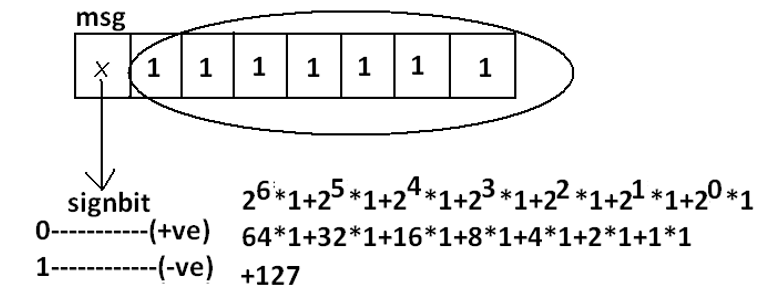
\includegraphics[scale=.4]{content/chapter2/images/byte.png}
		\end{figure}		
		\item Left most bit (also called \textbf{m}ost \textbf{s}ignificant \textbf{b}it) is sign bit , where 
		\begin{itemize}
			\item 0 is positive number
			\item 1 is negative number
		\end{itemize}
	
		\begin{figure}[h!]
			\centering
			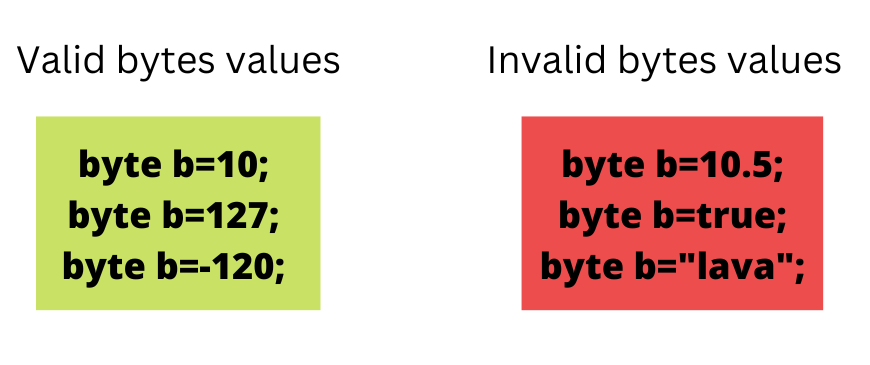
\includegraphics[scale=.45]{content/chapter2/images/byte2.png}
		\end{figure}		
		
	
		\item \textbf{Where is byte used?}
		\begin{itemize}
			\item \textbf{Reading and writing binary data}
			\item \textbf{Image processing}			
			\item \textbf{Audio processing}
			\item \textbf{Network programming}
		\end{itemize}	
	\end{itemize}
	
\end{flushleft}

\newpage


\subsection{short}


\begin{flushleft}
	\begin{itemize}
		\item Least frequently used data type.
		\item short keyword is 16-bit signed integer. 
		
		\tabletwo{
		\hline
		Size & \textbf{2 byte (16 bits)} \\
		\hline
		MAX\_VALUE & 32767 \\
		\hline
		MIN\_VALUE & -32768 \\
		\hline
		Range & \textbf{-$2^\textbf{15}$} to \textbf{$2^\textbf{15}$-1}  \\
		\hline
		}
		\bigskip
		\item \textbf{Where is short data type used?}
		\begin{itemize}
			\item Short data type used for 16 bit processor like 8085.
		\end{itemize}	
	
		\begin{figure}[h!]
			\centering
			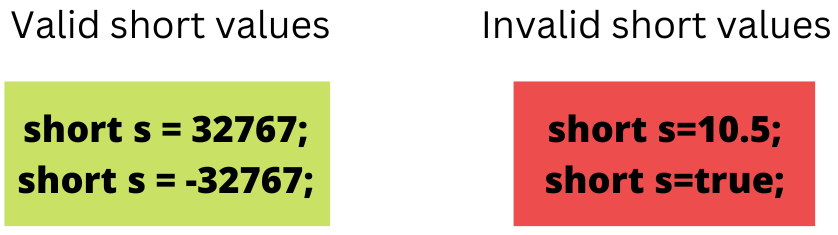
\includegraphics[scale=.38]{content/chapter2/images/short.png}
		\end{figure}		
	\end{itemize}
	
\end{flushleft}
\newpage

\subsection{int}


\begin{flushleft}
	
	\begin{itemize}
		\item Mostly commonly used data type is int.
		\item int keyword is 32-bit signed integer. 
		\tabletwo{
		\hline
		Size & \textbf{4 byte (32 bits)} \\
		\hline
		MAX\_VALUE & 2147483647 \\
		\hline
		MIN\_VALUE & -2147483648 \\
		\hline
		Range & \textbf{-$2^\textbf{31}$} to \textbf{$2^\textbf{31}$-1}  \\
		\hline
		}
		\bigskip
		
		\begin{figure}[h!]
			\centering
			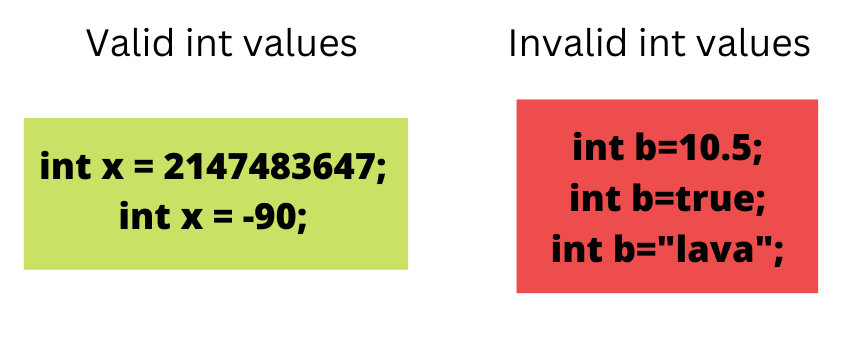
\includegraphics[scale=.45]{content/chapter2/images/int.png}
		\end{figure}		
		
		
	\end{itemize}
	
\end{flushleft}

\newpage


\subsection{long}


\begin{flushleft}
	
	\begin{itemize}
		\item long keyword is 64-bit signed integer. 
		
		\tabletwo{
			\hline
			Size & \textbf{8 byte (64 bits)} \\
			\hline
			MAX\_VALUE & $2^\textbf{63}$-1 \\
			\hline
			MIN\_VALUE & -$2^\textbf{63}$ \\
			\hline
			Range & \textbf{-$2^\textbf{63}$} to \textbf{$2^\textbf{63}$-1}   \\
			\hline
		}
		
		\bigskip
		\item \textbf{Where is long data type used?}
		\begin{itemize}
			\item Eg 1: Amount of distance travelled by light in 1,000 days. To hold this value integer is not enough. Hence, long is used.
			\newline
			long l = 1,26,000 X 60 X 60 X 24 X 1000 miles.
			\bigskip
			\item Eg 2: The number of characters present in a big file may exceed int range. Hence, the return type of length() is long but not integer. 
			\codeblock{
				long l = f.length()
			}
			
		\end{itemize}	
	
		\bigskip
		\textbf{Long literals}
		\begin{itemize}
			\item \textbf{long} data type can be suffixed with "l" or "L".
			
			\item Below are valid \textbf{long} data type:
			\codeblock{
				long l = 10L; \cmark \\
				long b = 10; \cmark
			}
			
			\item However, below declaration will result in error:
			\codeblock{
					int x = 10L; \xmark
			}

		\end{itemize}
		
		
	\end{itemize}
	
\end{flushleft}

\newpage


\subsection{Integer literals}

\begin{flushleft}
	
	\begin{itemize}
		\item For integral datatypes like byte, short, int \& long, we can specify literal value in the following base:
		\begin{itemize}
			\item \textbf{Decimal literal (base-10)}:
			\begin{itemize}
				\item Allowed digits are 0-9
				\codeblock{
					int x = 10;
				}
			\end{itemize}

		\item \textbf{Binary literal (base-2)}:
		\begin{itemize}
			\item From Java 1.7 version, integral literal can be represented as binary value.
			\item Allowed digits are 0 and 1
			\item Literal value should be pre-fixed with "0B" or "0b"
			\codeblock{
				int x = 0B10; \newline
				int y = 0b10101;
			}
		\end{itemize}

			
		\item \textbf{Octal literal (base-8)}:
		\begin{itemize}
			\item Allowed digits are 0-7
			\item Literal value should be pre-fixed with 0
			\codeblock{
					int x = 017;
			}
		\end{itemize}
	
		\item \textbf{Hexadecimal literal (base-16)}:
		\begin{itemize}
			\item Allowed digits are 0-9, a-f or A-F
			\item Literal value should be pre-fixed with "0X" or "0x"
			\codeblock{
				int x = 0X13aA; \\
				int x = 0x45Fe;
			}
		\end{itemize}

		\item \textbf{Usage of \_ in numeric literal}:
		\begin{itemize}
			\item From Java 1.7 version, we can use "\_" in middle of big numbers to increase integer's readability.
			\item At the time of compilation, these "\_" symbols will be removed automatically.
			\bigskip
			\codeblock{
				int x = 78\_32\_34\_23; \newline
				int y = 0Xaa\_ff\_11; \newline
				int z = 034\_12\_10; \newline
				int a = 0B11\_\_00\_10\_11;
			}
			\item "\_" symbol cannot be used in the starting or end of integer. Below are \textbf{invalid} declarations:
			\bigskip
			\codeblock{
				int x = \_78\_32\_34\_23; \newline
				int y = 0Xaa\_ff\_11\_; 
			}
						
			
		\end{itemize}
	\end{itemize}
		
	\end{itemize}

	\newpage
	\textbf{Program to convert octal and hexadecimal form of integer to decimal form:}

	\codeblockfull{test.java}{
		package Starter; \newline
		class test \newline
		\{ \newline
		\s	public static void main (String[] args) \newline
		\hphantom{} \hphantom{}	\{ \newline
		\hphantom{} \hphantom{} \hphantom{} \hphantom{}	int x = 10; \newline
		\hphantom{} \hphantom{} \hphantom{} \hphantom{}	int y = 061; \newline
		\hphantom{} \hphantom{} \hphantom{} \hphantom{} int z = 0x9a; \newline
		\hphantom{} \hphantom{} \hphantom{}	\hphantom{}	System.out.println(x+","+y+","+z); \newline
		\hphantom{} \hphantom{}	\} \newline
		\} 	
	}
	\outputblock{
		10,49,154
	}

	\textbf{Output Explaination:}
	
	In Java, integeral literals are always represents in decimal literals forms: 
			\begin{itemize}	
				\item Octal to decimal form: 
					\[ (61)_8 = (?)_{10} \]
					\[ 6 \times 8^{1} + 1 \times 8^{0} = 49  \]
				\item Hexadecimal to decimal form:
					\[ (9a)_{16} = (?)_{10} \]
					\[ 9 \times 16^{1} + 10 \times 16^{0} = 154  \]
			\end{itemize}
			
\end{flushleft}

\newpage


\section{Floating-point}


\begin{flushleft}
	
	Floating-point numbers, also known as real numbers.
	There are two kinds of floating-point type:
	
	\newimage{0.5}{content/chapter0/images/new30.png}
	
		
\end{flushleft}


\subsection{Float}


\begin{flushleft}
	
	\begin{itemize}
		\item Represent \textbf{single-precision} numbers (upto 7 decimal digits)
		
		\tabletwo{
			\hline
			Size & \textbf{4 byte (32 bits)} \\
			\hline
			MAX\_VALUE & 3.4e38 \\
			\hline
			MIN\_VALUE & -3.4e38 \\
			\hline
			Range & -3.4e38 to 3.4e38   \\
			\hline
		}
		
	\end{itemize}
		
\end{flushleft}


\subsection{Double}


\begin{flushleft}
	
	\begin{itemize}
		\item Represent \textbf{double-precision} numbers (upto 16 decimal digits)
		
		\tabletwo{
			\hline
			Size & \textbf{8 byte (64 bits)} \\
			\hline
			MAX\_VALUE & 1.7e+308 \\
			\hline
			MIN\_VALUE & 1.7e-308 \\
			\hline
			Range & 1.7e-308 to 1.7e+308   \\
			\hline
		}
		
	\end{itemize}
		
\end{flushleft}

\newpage


\subsection{Floating-point literals}

\begin{flushleft}

	\begin{itemize}
		
		\item By default, floating-point numbers are represented in double form.
		\item So below declaration will result in error: 
		\bigskip		
		\codeblock{
				float f = 1.0 \xmark
		}
		\bigskip		
		
		\item Correct way to represent float data type is by suffixing \textbf{"F"} or \textbf{"f"} to the floating-point number as shown:
		\bigskip
		\codeblock{
			float f = 1.6F; \cmark \newline
			float f = 7.8f;		\cmark
		}

		\item Double data type can be represented using suffix \textbf{"D"} or \textbf{"d"} or no suffix as below:
		\bigskip
		\codeblock{
		    double a = 12.67; \cmark \newline
			double b = 13.7d; \cmark \newline
			double c = 123.456D; \cmark 
		}
	
		\item Assign integral literal directly to floating-point variables:
		\bigskip
		\codeblock{
			double a = 0456; \cmark \newline
			float b = 0XFace; \cmark 
		}
			
		\item \textbf{Expontential format:} This is scientific notation to represent very large or small floating-point values. Use the letter “e” or “E” to indicate the exponent:
				\bigskip
		\codeblock{
			double a = 1.2e3; \cmark \newline
			float b = 1.3e4F; \cmark
		}
		
		\bigskip
		\item \textbf{Usage of \_ in floating literal}:
		\begin{itemize}
			\item From Java 1.7 version, "\_" in middle of big numbers increase floating-point's readability:
			\codeblock{
				double y = 12\_45\_23\_\_23\_2323.90;  \cmark
			}
						
		\end{itemize}	
		
	\end{itemize}
	
\end{flushleft}



\section{Character}


\begin{flushleft}
	
	\begin{itemize}
		\item In order to understand char data type, we need to understand what is "ASCII" and "UNICODE"
		
	\end{itemize}
	
\end{flushleft}



\subsection{What is ascii \& unicode?}


\begin{flushleft}
	
	\begin{itemize}
		\item \textbf{ASCII (American Standard Code for Information Interchange)}:
		\begin{itemize}
			\item Is a character encoding system that \textbf{represents text in computers}.
			\item It uses a 7-bit code to represent 128 characters, including the letters of the English alphabet, digits, punctuation marks, and some control codes.
			\newimage{0.45}{content/chapter0/images/new31.png}
			\newimage{0.3}{content/chapter0/images/ascii.png}
			
		\end{itemize}
		
		\newpage
		
		\item \textbf{Unicode}:
		\begin{itemize}
			\item It is a character encoding standard designed to support the representation of \textbf{all the world's languages}.

		\end{itemize}  
				
	\end{itemize}
	
\end{flushleft}



\subsection{char datatype}


\begin{flushleft}
	
	\begin{itemize}
		\item Java \textbf{uses unicode} to represent \textbf{char datatype}. 
		\item There are \textbf{no negative chars}.
		\item Character is represented in \textbf{single quotes}.

		\tabletwo{
			\hline
			Size & \textbf{2 byte (16 bits)} \\
			\hline
			MAX\_VALUE &  65,535 \\
			\hline
			MIN\_VALUE & 0 \\
			\hline
			Range & 0 to 65,535 \\
			\hline
		}
		\bigskip
		
		Eg:
		\codeblock{
			class New \{ \\
			\s	public static void main(String[] args) \{ \\
			\s \s		char a = 88; \\
			\s \s		char b = 'x'; \\
			\s \s		System.out.println(a); \\
			\s \s		System.out.println(b); \\
			\s	\} \\
			\}
		}				
		
		
	\end{itemize}
	
\end{flushleft}

\newpage


\subsection{Character literals}

\begin{flushleft}
	\begin{itemize}		
		\item Char literal can be represented as \textbf{single character within single quotes}.
		\codeblock{
			char ch='a'; \cmark
		}

		\item Below char literal declaractions will \textbf{result into compile time errors}:
		
		\codeblock{
			char ch = "a"; \xmark \\
			char ch = a; \xmark \\
			char ch = 'ab'; \xmark 
		}

		\item Char literal can also be \textbf{represented as integral literal} which represents the unicode value of character.
		\newline
		The unicode value can be specified in decimal, octal and hexa decimal form.
		\codeblock{
			char ch1 = 97; \cmark \\
			char ch2 = 0xFace; \cmark \\
			char ch3 = 0777; \cmark \\
			char ch = 65535; \cmark
		}

		Note that allowed range is \textbf{0 to 65535}.
		
		\bigskip
		\item Char literal can also be represented in \textbf{unicode representation} by using "\textbackslash uXXXX" syntax where "XXXX" is 4 digit hexa decimal number.
		
		\codeblock{
			char ch1 = '\textbackslash u0052'; \cmark \\
			char ch2 = '\textbackslash u0932'; \cmark \\
			char ch3 = \textbackslash uface; \cmark
		}
		
		\newpage
		
		\item Char literal can also \textbf{represent escape sequence characters}.
		\codeblock{
			char ch1 = '\textbackslash n';  \cmark \\
			char ch2 = '\textbackslash t'; \cmark
		}

	\end{itemize}
	

\end{flushleft}




\subsection{Escape character}

\begin{flushleft}
	
	A character preceded by a backslash (\textbackslash) is an escape sequence and has special meaning to the compiler. 
	\newline
	The following table shows the Java escape sequences:
	
	\begin{tabulary}{1.0\textwidth}{|p{12em}|p{12em}|}
		\toprule
		\textbf{Escape Character} & \textbf{Decimal Point} \\
		\midrule
		\textbackslash n & New line \\
		\hline
		\textbackslash t & Horizontal Tab \\
		\hline
		\textbackslash r & Carriage return (Move to first character in next line) \\
		\hline
		\textbackslash b & Back Space \\
		\hline
		\textbackslash f & form feed \\
		\hline
		\textbackslash ' & single quote \\
		\hline
		\textbackslash " & double quote \\
		\hline
		\textbackslash \textbackslash & Back Slash \\
		\bottomrule
	\end{tabulary}

	Eg:
	
	\codeblock{
		System.out.println("This is line one \textbackslash n And this is line two"); \newline
		System.out.println("This is \textbackslash t tab space"); \newline
		System.out.println("Sunflower \textbackslash r Forest");  \newline
		System.out.println("Sunflower \textbackslash f Forest \textbackslash f ground"); \newline
		System.out.println("C:\textbackslash\textbackslash lavatech\_technology"); \newline
		System.out.println("Sunflower\textbackslash 's Forest"); 
	}

\end{flushleft}

\newpage


\section{Boolean}


\begin{flushleft}
	
	\begin{itemize}
		\item Boolean is datatype for logical values. 
		\item Boolean is return by all relational operators.

	\end{itemize}
		
		\tabletwo{
			\hline
			Size & \textbf{1 byte (8 bits)}. The actual memory usage may depend on JVM implementation. \\
			\hline
			Value & true, false \\
			\hline
		}

		\begin{figure}[h!]
			\centering
			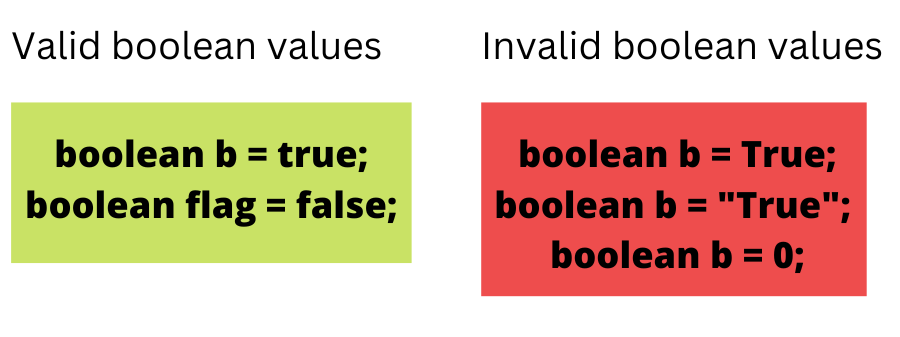
\includegraphics[scale=.35]{content/chapter2/images/boolean.png}
		\end{figure}		
				
		\noteblock{
			\begin{itemize}
				\item The values of true and false do not convert into any numerical representation. 
				\item The true literal in Java does not equal 1, nor does the false literal equal 0. 
			\end{itemize}
		}
		\begin{figure}[h!]
			\centering
			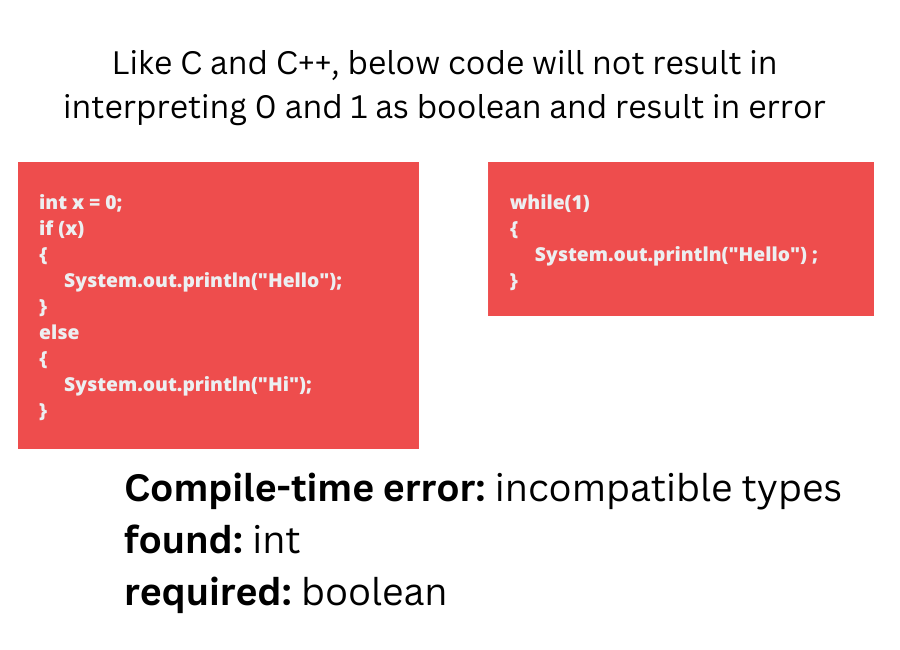
\includegraphics[scale=.45]{content/chapter2/images/bool.png}
		\end{figure}		
				
		
		

	
\end{flushleft}

\newpage


\section{Type conversion}


\begin{flushleft}

	
	Converting one primitive data type into another is known as type conversion. There are two types of type conversions:

	
	\begin{itemize}

		\item \textbf{Implicit type casting or widening:} 
		\begin{itemize}
			\item \textbf{Converting a lower datatype to a higher datatype} is known as widening or up-casting.
			\item Compiler is responsible to perform implicity type casting.
			\item There is no loss of information in this type casting.
			\item The following are various possible conversions:
		\end{itemize}
		

		
		\begin{figure}[h!]
			\centering
			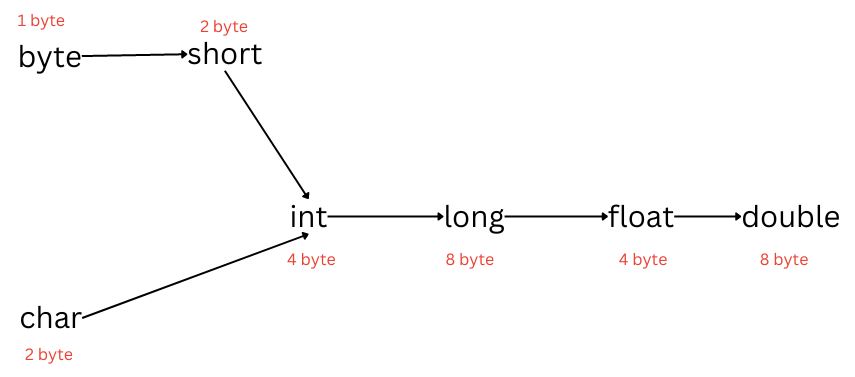
\includegraphics[scale=.4]{content/chapter2/images/convert.png}

		\end{figure}		
		Eg:
		\codeblock{
			int x = 'a';  \\
			System.out.println(x);    // output: 97 \\
			\\
			double d = 10; \\
			System.out.println(d);  // output: 10.0
		}
	
		\bigskip
		\noteblock{
			\begin{itemize}
				\item \textbf{Long value can be assigned to float variable} because both are following different memory representations internally. 
			\end{itemize}
		}
		
		
		\newpage
		
		\item \textbf{Explicit type casting or narrowing:} 
		\begin{itemize}
			\item Converting a higher datatype to a lower datatype is known as narrowing or down casting.
			\item Programmer is responsible to perform explicit type casting.
			\item Loss of information is possible.
			\item The following are various possible conversions:
			
			\newimage{0.5}{content/chapter2/images/rev.png}
			
			\item Except for boolean, all datatypes can be type-cast to other primitive data-type.
			\item Type-cast operator for each primitive datatype:
			
		\end{itemize}
		
		\tablethree{
			\hline
			Data type & Type-case operator & Example \\
			\hline
			byte & (byte) &  double d = 130.4; \newline byte x = (byte) d; \\
			\hline
			short & (short) & double d = 130.4; \newline short x = (short) d; \\
			\hline
			int & (int) & double d = 130.4; \newline int x = (int) d; \\
			\hline
			long & (long) & double d = 130.4; \newline long x = (long) d; \\
			\hline
			float & (float) & double d = 130.4; \newline float x = (float) d; \\
			\hline
			double & (double) & float d = 130.4; \newline double x = (double) d; \\
			\hline
			char & (char) & double d = 130.4; \newline char x = (char) d; \\
			\hline
		}
		
		Eg 1:
		\codeblock{
			int x = 130; \\
			//byte b = x;      \xmark \\
			byte b = (byte) x;  \cmark    \\
			System.out.println(b);   // output: -126
		}
	
		Output explaination:
		\begin{itemize}
			\item Integer is 32-bit in size \& byte is 8-bit in size.
			\item 32-bit binary representation of 130 is 0000000…10000010.
			\item To convert integer to byte datatype, mean downsize decimal representation of 130 to fit in 8 bit.
			\item Which means the binary number \textbf{0000000…10000010} is down-sized to \textbf{10000010}
			\item Note that left-most bit is "1" and hence number is now represented as 2's complement.
			\item 2's complement of \textbf{10000010} is \textbf{11111101+1 => 11111110 => -126}
		\end{itemize}

		\bigskip

		Eg 2: If we assign floating point values to integral types, by explicit type casting, the digits after decimal point will be lost.
		\bigskip
		\codeblock{
			double d = 130.456; \\
			int x = (int) d;  \\
			System.out.println(x); // output: 130 \\
			\\
			byte b = (byte) d;  \\
			System.out.println(b);  // output: -126
		}
		
	\end{itemize}
	
\end{flushleft}


\newpage




%-----------------------

%-------------------------------------------------------------------------------------
%	CHAPTER 4
%-------------------------------------------------------------------------------------
\chapterimage{index5.png} % Table of contents heading image
\chapter{Arrays}
%-----------------------
\section{Arrays in detail}
\setlength{\columnsep}{3pt}
\begin{flushleft}
	\bigskip
	\bigskip
		In this section, you are going to learn:	\newimage{0.68}{content/chapter4/images/loop.png}

	
	
\end{flushleft}

\newpage


\subsection{Array introduction}
\setlength{\columnsep}{3pt}
\begin{flushleft}
	\bigskip
	An array is \textbf{indexed collection of fixed number of homogeneous data elements}.
	
	\bigskip\bigskip
	\begin{figure}[h!]
		\centering
		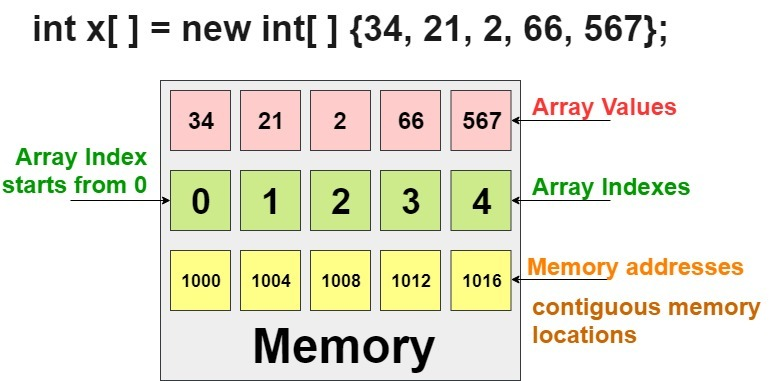
\includegraphics[scale=.45]{content/chapter4/images/array.jpg}
	\end{figure}		
	
	\textbf{Advantage}:
	\begin{itemize}
		\item Array can represent huge number of values using single variable that will improve readability of code.
	\end{itemize}
	
	\textbf{Disadvantage}:
	\begin{itemize}
		\item Array are fixed in size.
		\item Once an array is created, they cannot be increased or decreased.
		\item Array size need to be mentioned in advance, which is not always possible.
	\end{itemize}
	
	
\end{flushleft}





\subsection{Array declaration}
\setlength{\columnsep}{3pt}
\begin{flushleft}
	\begin{itemize}
		\item \textbf{One dimensional array declaration}:
		\bigskip
		\syntaxblock{
			int[] x; (Recommended as name of variable is clearly separated from type) \newline
			int []x; \newline
			int x[];
		}
		\bigskip
		\noteblock{
			Array declaration \textbf{cannot define size} of array.
			\codeblock{
				int[6] x; \xmark
			}
		}
		
		\bigskip
		\item \textbf{Two-dimensional array declaration}:
		\bigskip
		\syntaxblock{
			int[][] x;  (Recommended)
			\newline
			int [][]x;
			\newline
			int x[][];
		}
		
		
		\newpage
		\item \textbf{3-dimensional array declaration:}
		\bigskip
		\syntaxblock{
			int[][][] x;  (Recommended)
			\newline
			int [][][]x;
			\newline
			int x[][][];
		}
		
		\bigskip		
		\item \textbf{More combinations}:
		\begin{itemize}
			\item Declaring variable \textbf{"a"} and \textbf{"b"} with \textbf{1} dimension:
			\bigskip
			\codeblock{
				int[] a,b;
			}
			\bigskip
			\item Declaring variable \textbf{"a"} with 2 dimension and variable \textbf{"b"} with 1 dimension
			\bigskip
			\codeblock{
				int[] a[],b;
			}
			
			\item Declaring variable \textbf{"a"} and \textbf{"b"} with 2 dimensions.
			\bigskip
			\codeblock{
				int[] a[],b[]; \\
				int[] \s a[],b;
			}
			
			\item Declaring variable \textbf{"a"} with 2 dimension and variable \textbf{"b"} with 3 dimension:
			\codeblock{
				int[] \s []a,b[];
			}		
			
			\bigskip
			\noteblock{
				\textbf{"[]" is allowed only in front of first variable.} 
				\codeblock{
					int[] \hphantom{} \hphantom{} []a,[]b; \xmark  \\
					int[] \hphantom{} \hphantom{} []a,[]b,[]c; \xmark
				}
			}
			
		\end{itemize}
		
	\end{itemize}
	
	
	
\end{flushleft}

\subsection{Array creation}
\setlength{\columnsep}{3pt}
\begin{flushleft}
	\bigskip
	
	Things to note about array:
	\begin{itemize}
		\item In Java, every array is an Object.
		\item \textbf{"new"} operator is used to create an object.
		\item Hence, we can create array by using \textbf{new} operator.
	\end{itemize}
	
	
	\begin{itemize}
		
		\item \textbf{One dimensional array creation}:
		
		\begin{tcolorbox}[breakable,notitle,boxrule=1pt,colback=pink,colframe=pink]
			\color{black}
			\fontdimen2\font=8pt
			Syntax:  \newline
			int[] a = new int[4];
			\fontdimen2\font=4pt
		\end{tcolorbox}
		
		
		\begin{figure}[h!]
			\centering
			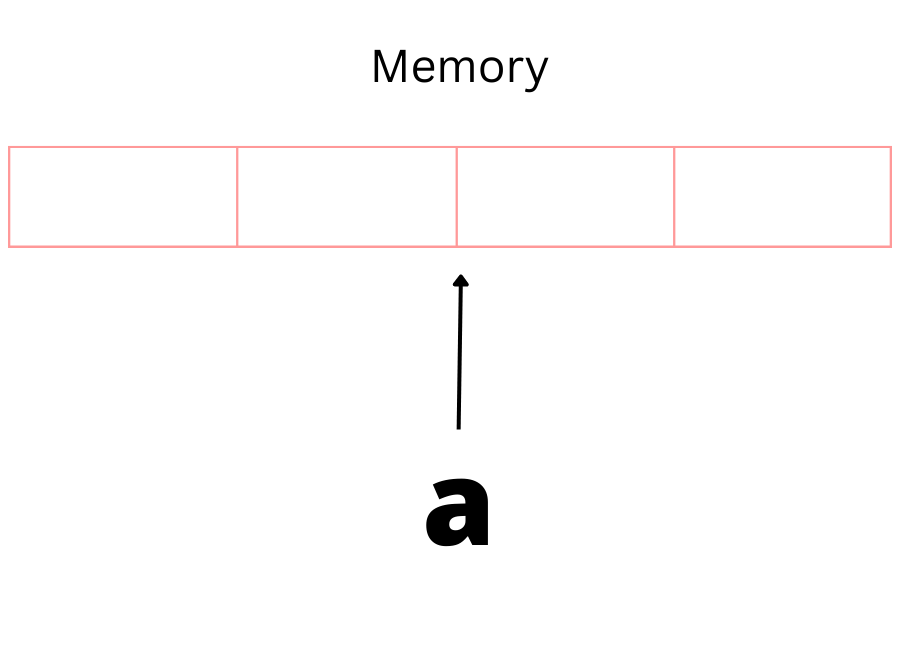
\includegraphics[scale=.45]{content/chapter4/images/array.png}
		\end{figure}	
		
		Important:
		\begin{itemize}
			\item At the time of array creation, \textbf{size should be mentioned compulsorily.}
			\item An array can be of zero size.
			\begin{tcolorbox}[breakable,notitle,boxrule=-0pt,colback=code,colframe=code]
				\color{black}
				\fontdimen2\font=8pt
				int[] x = new int[]; \xmark \par
				int[] x = new int[6]; \cmark  \par
				int[] x = new int[0]; \cmark 
				\fontdimen2\font=4pt
			\end{tcolorbox}
			
			\item Java compiler will never throw error for negative size of array. However, Java Virtual Machine will throw runtime error: \textbf{NegativeArraySizeException}.
			\begin{tcolorbox}[breakable,notitle,boxrule=-0pt,colback=code,colframe=code]
				\color{black}
				\fontdimen2\font=8pt
				int[] x = new int[-3]; \xmark
				\fontdimen2\font=4pt
			\end{tcolorbox}
			
			\item Allowed data types for mentioning array size are:
			\begin{itemize}
				\item integer
				\item byte
				\item short
				\item char
			\end{itemize}
			
			\begin{figure}[h!]
				\centering
				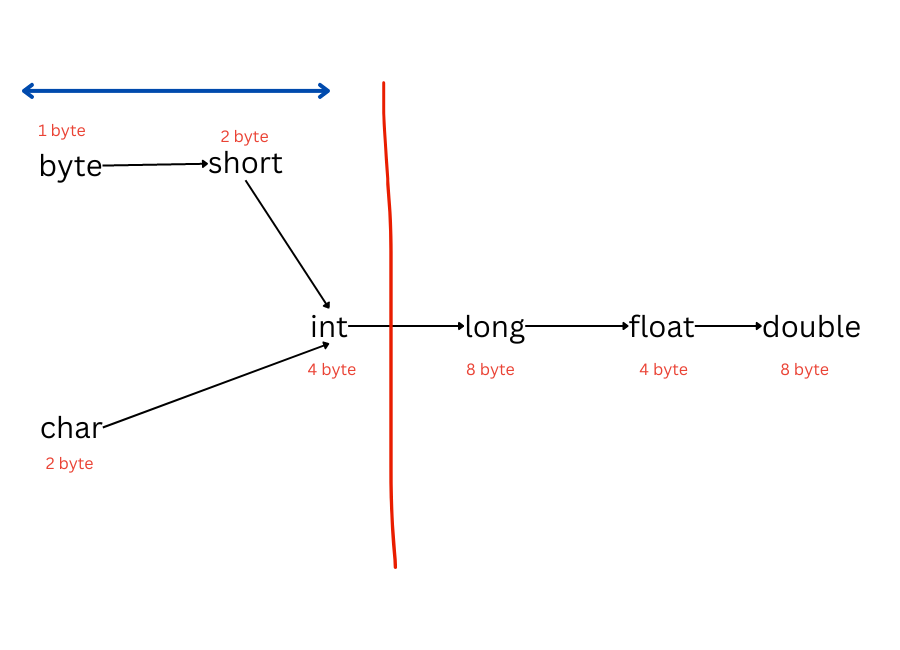
\includegraphics[scale=.45]{content/chapter4/images/allow.png}
			\end{figure}	
			
			\begin{tcolorbox}[breakable,notitle,boxrule=-0pt,colback=code,colframe=code]
				\color{black}
				\fontdimen2\font=8pt
				int[] x = new int[10]; \cmark \par
				int[] x = new int['a']; \cmark \par
				byte b = 20; \par
				int[] x = new int[b]; \cmark \par
				short s = 30; \par
				int[] x = new int[s]; \cmark \par
				\fontdimen2\font=4pt
			\end{tcolorbox}
			
			\newpage
			Below array creation will result in error:
			\begin{tcolorbox}[breakable,notitle,boxrule=-0pt,colback=code,colframe=code]
				\color{black}
				\fontdimen2\font=8pt
				int[] x = new int[10l]; \xmark \par
				int[] x = new int[3.5]; \xmark 
				\fontdimen2\font=4pt
			\end{tcolorbox}
			
			\item Maximum size of array can be 2147483647:
			\begin{tcolorbox}[breakable,notitle,boxrule=-0pt,colback=code,colframe=code]
				\color{black}
				\fontdimen2\font=8pt
				int[] x = new int[2147483647]; \cmark \par
				int[] x = new int[2147483648]; \xmark 
				\fontdimen2\font=4pt
			\end{tcolorbox}
			
			\item For every array type, corresponding classes are available and these classes are part of Java language and not available to the programmer level.
			\bigskip
			\bigskip
			\begin{tabulary}{1.0\textwidth}{|p{12em}|p{12em}|}
				\toprule
				\textbf{Array type} & \textbf{Corresponding class name} \\
				\midrule
				int[] & [I \\
				\hline
				int[][] & [[I \\
				\hline
				double[] & [D \\
				\hline
				short[] & [S \\
				\hline
				byte[] & [B \\
				\hline
				boolean[] & [Z \\
				\bottomrule
			\end{tabulary}
			\bigskip
			Eg: You can find name of class for different array type:
			\begin{tcolorbox}[breakable,notitle,boxrule=-0pt,colback=code,colframe=code]
				\color{black}
				\fontdimen2\font=8pt
				int[] a = new int[3]; \newline
				System.out.println(a.getClass().getName());
				\fontdimen2\font=4pt
			\end{tcolorbox}
			
			Output:
			\begin{tcolorbox}[breakable,notitle,boxrule=-0pt,colback=output,colframe=output]
				\color{black}
				\fontdimen2\font=8pt
				[I			
				\fontdimen2\font=4pt
			\end{tcolorbox}	
			
			
		\end{itemize}
		
		\newpage
		\item \textbf{Two-dimensional array creation}:
		\begin{itemize}
			\item In Java, two dimensional array is not implmeneted using matrix approach.
			\item Array of arrays approach is followed for multi-dimensional array creation.
			\item Advantage of array of arrays approach is improved memory utilisation.
			
			
		\end{itemize}
		\bigskip
		
		There are different ways of creating two-dimensional array.
		\begin{itemize}
			\item \textbf{Base size}: In this we specifiy the size of first dimension at the time of array creation.
			\begin{tcolorbox}[breakable,notitle,boxrule=-0pt,colback=code,colframe=code]
				\color{black}
				\fontdimen2\font=8pt
				int[][] x = new int[2][]; \par
				x[0] = new int[2]; \par
				x[1] = new int[3];
				\fontdimen2\font=4pt
			\end{tcolorbox}
			
			\begin{figure}[h!]
				\centering
				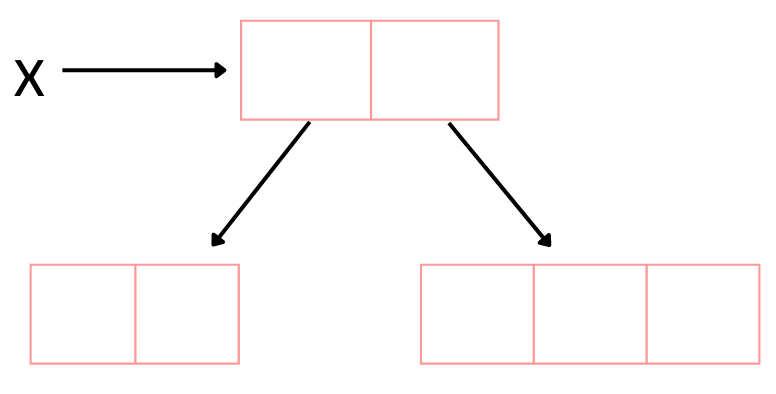
\includegraphics[scale=.45]{content/chapter4/images/two.png}
			\end{figure}	
			
			\newpage
			
		\end{itemize}
		
		\item Three-dimensional array creation:
		\begin{tcolorbox}[breakable,notitle,boxrule=-0pt,colback=code,colframe=code]
			\color{black}
			\fontdimen2\font=8pt
			int[][][] x = new int[2][][]; \par
			x[0] = new int[3][]; \par
			x[0][0] = new int[1]; \par
			x[0][1] = new int[2]; \par
			x[0][2] = new int[3]; \par
			x[1] = new int[2][2];
			\fontdimen2\font=4pt
		\end{tcolorbox}
		
		\begin{figure}[h!]
			\centering
			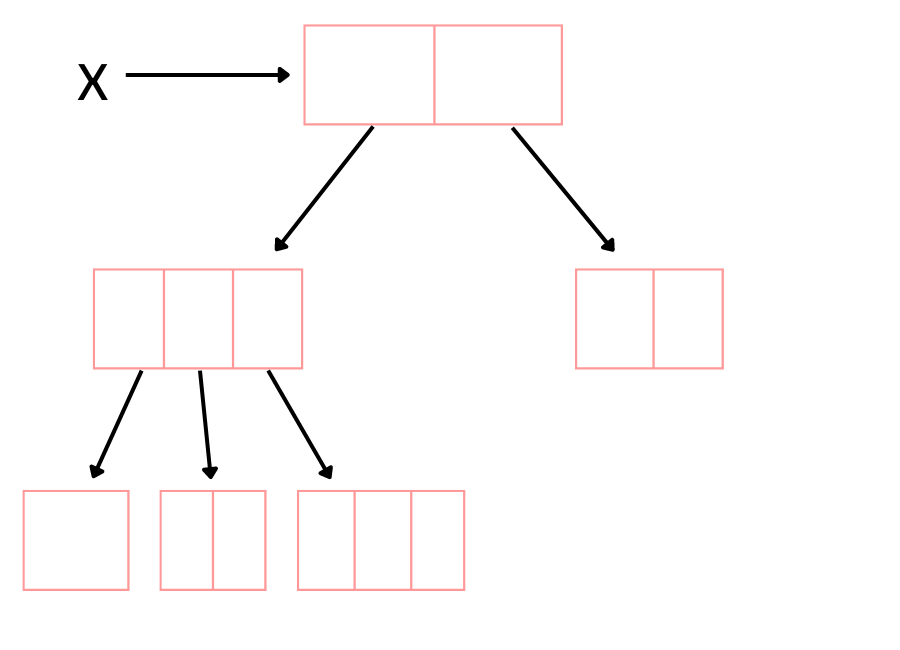
\includegraphics[scale=.45]{content/chapter4/images/three.png}
		\end{figure}
		
		
	\end{itemize}
	
	
	
\end{flushleft}

\newpage





%\subsection{Practice}
%\setlength{\columnsep}{3pt}
\begin{flushleft}
	\paragraph{}
	
	\bigskip
	
	\begin{figure}[h!]
		\centering
		
\includegraphics[scale=.2]{content/practise.jpg}
	\end{figure}	
	
	
	
\end{flushleft}
\newpage



\subsection{Array initialisation}
\setlength{\columnsep}{3pt}
\begin{flushleft}
	\bigskip
	\begin{itemize}
		\item \textbf{One dimensional array}:\par
		
		Once we create an array, every array element is by default initialized with default values.
		
		\begin{figure}[h!]
			\centering
			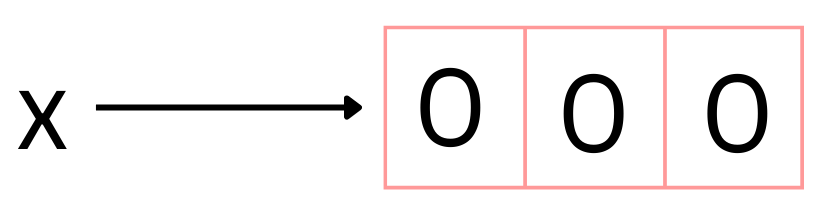
\includegraphics[scale=.45]{content/chapter4/images/new1.png}
		\end{figure}	
		
		
		\begin{tcolorbox}[breakable,notitle,boxrule=1pt,colback=code,colframe=code]
			\color{black}
			\fontdimen2\font=8pt
			int[] a = new int[3]; \par
			System.out.println(a); \par
			System.out.println(a[0]);
			\fontdimen2\font=4pt
		\end{tcolorbox}
		
		Output:
		\begin{tcolorbox}[breakable,notitle,boxrule=-0pt,colback=output,colframe=output]
			\color{black}
			\fontdimen2\font=8pt
			[I@422a8473 \par
			0
			\fontdimen2\font=4pt
		\end{tcolorbox}	
		
		Whenever we are trying to print any reference variable, internally two string method will be called, which is implemented by default to return the string in the following form:
		\par
		\textbf{class\_name@hexadecimal\_form}
		
		\bigskip
		\item \textbf{Two-dimensional array}:  \par
		
		Example 1:
		\begin{figure}[h!]
			\centering
			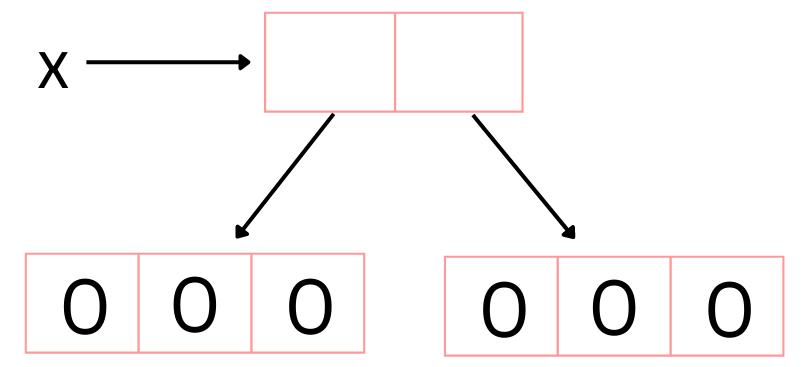
\includegraphics[scale=.45]{content/chapter4/images/new2.png}
		\end{figure}	
		
		\begin{tcolorbox}[breakable,notitle,boxrule=1pt,colback=code,colframe=code]
			\color{black}
			\fontdimen2\font=8pt
			int[][] a = new int[2][3]; \par
			System.out.println(a);  \par
			System.out.println(a[0]);  \par
			System.out.println(a[0][0]);			
			\fontdimen2\font=4pt
		\end{tcolorbox}
		
		Output:
		\begin{tcolorbox}[breakable,notitle,boxrule=-0pt,colback=output,colframe=output]
			\color{black}
			\fontdimen2\font=8pt
			[[I@5a39699c \par
			[I@129a8472  \par
			0
			\fontdimen2\font=4pt
		\end{tcolorbox}	
		
		Example 2:
		
		\begin{figure}[h!]
			\centering
			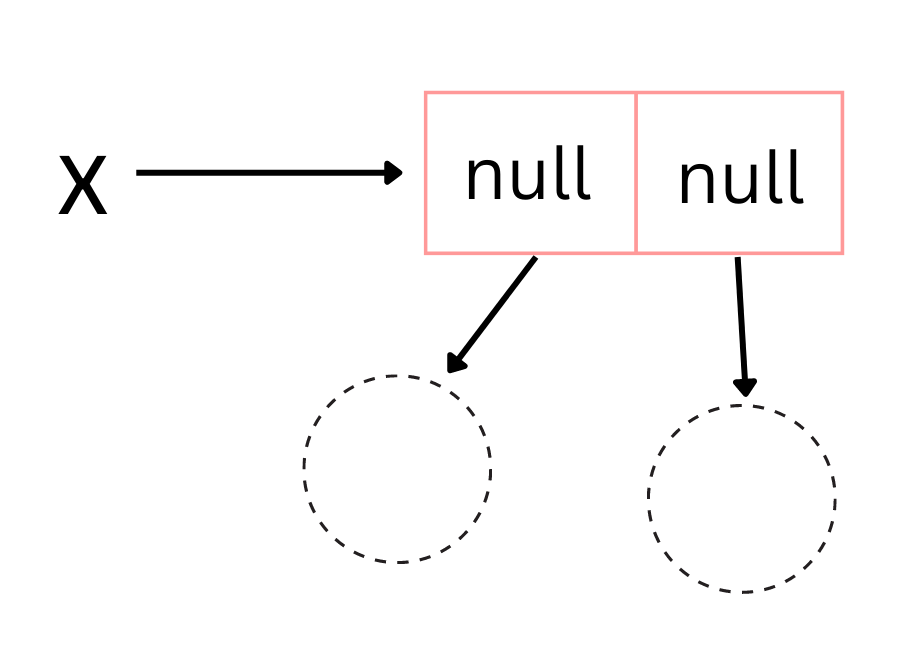
\includegraphics[scale=.45]{content/chapter4/images/new3.png}
		\end{figure}	
		
		\begin{tcolorbox}[breakable,notitle,boxrule=1pt,colback=code,colframe=code]
			\color{black}
			\fontdimen2\font=8pt
			int[][] a = new int[2][]; \par
			System.out.println(a);  \par
			System.out.println(a[0]);  \par
			System.out.println(a[0][0]);			
			\fontdimen2\font=4pt
		\end{tcolorbox}
		
		Output:
		\begin{tcolorbox}[breakable,notitle,boxrule=-0pt,colback=output,colframe=output]
			\color{black}
			\fontdimen2\font=8pt
			[[I@5a39699c \par
			null  \par
			Exception in thread "main" java.lang.NullPointerException: 
			\fontdimen2\font=4pt
		\end{tcolorbox}	
		
		\bigskip
		
		\item \textbf{Over-riding array value:} \par
		Once we create an array, every array element by default initialised with default values. \par
		We can over-ride default values with custom values.
		
		\begin{figure}[h!]
			\centering
			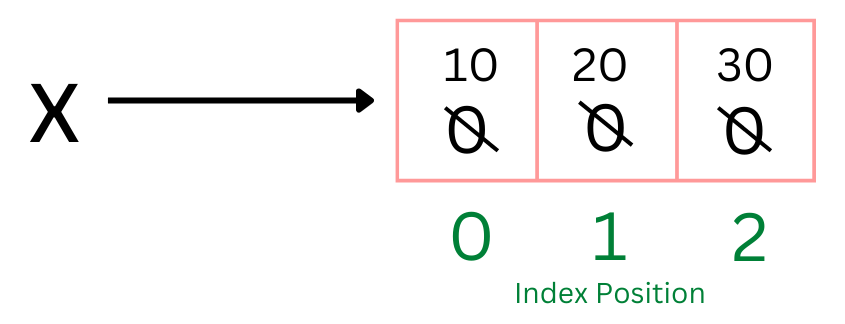
\includegraphics[scale=.45]{content/chapter4/images/image2.png}
		\end{figure}	
		
		\begin{tcolorbox}[breakable,notitle,boxrule=1pt,colback=code,colframe=code]
			\color{black}
			\fontdimen2\font=8pt
			int[] a = new int[3]; \par
			a[0]=10; \par
			a[1]=20; \par
			a[2]=30; \par
			System.out.println(a[0]); \par
			System.out.println(a[1]); \par
			System.out.println(a[2]);
			\fontdimen2\font=4pt
		\end{tcolorbox}
		
		Output:
		\begin{tcolorbox}[breakable,notitle,boxrule=-0pt,colback=output,colframe=output]
			\color{black}
			\fontdimen2\font=8pt
			10 \par
			20 \par
			30 
			\fontdimen2\font=4pt
		\end{tcolorbox}	
		
		Note: Trying to access array element with out of range index (either positive or negative integer value) will result in runtime exception:  \textbf{"ArrayINdexOutOfBoundException"}
		
	\end{itemize}
	
	
\end{flushleft}
\newpage


\subsection{Array declaration, creation and initialisation in one line}
\setlength{\columnsep}{3pt}
\begin{flushleft}

	\begin{itemize}
		\item \textbf{One dimensional array}:\par

		We can declare, create and initialise an array in a single line (shorcut representation):
		
		\newimage{0.55}{content/chapter4/images/a2.png}
		
		\codeblock{
			int[] x = \{10,20,30\}; \par
			char[] ch = \{'a','e','i','o','u'\}; \par
			String[] a = \{"Ram" , "Ravi"\};
		}
	
		You can declare the array \& provide it's value as shown below:
		\bigskip
		\codeblock{
			int[] x;     \\
			x = \{10,20,30\}; 
		}

		\bigskip
	
		\item \textbf{Multi-dimensional array}:
		
		\newimage{0.35}{content/chapter4/images/multi.png}

		\codeblock{
			int[] x = \{ \{ 10, 20 \}, \{ 30, 40, 50 \}  \};
		}	
				
		
		
	\end{itemize}
		
	
\end{flushleft}
\newpage



\subsection{length variable}
\setlength{\columnsep}{3pt}
\begin{flushleft}
	
	\textbf{length variable}:
	\begin{itemize}
		\item length is final variable applicable for arrays.
		\item length variable is used to display size of an array.
		\item Value returned by length is fixed as array once created cannot change it's size.
		\bigskip
		\codeblock{
			int[] x = new int[6]; \\
			System.out.println(x.length);  \cmark
		}
		\bigskip
		\outputblock{
			6
		}
		
		\item length variable is \textbf{not} applicable on string objects.
		\bigskip
		\codeblock{
			String s="lavatech"; \\
			System.out.println(s.length); \xmark
		}
		
		\item In multi-dimensional arrays, length variable represents only base size, but not total size.
		\codeblock{
			int[][] x = new int[6][3]; \\
			System.out.println(x.length);
		}
		\bigskip
		\outputblock{
			6
		}
		
	\end{itemize}
	
	\textbf{length()}:
	\begin{itemize}
		\item length() is present in String class.
		\item length() method is final variable applicable for string objects.
		\item It returns number of characters present in the string.
		\bigskip
		\codeblock{
			String s="lavatech"; \\
			System.out.println(s.length()); \cmark
		}
		\bigskip
		\outputblock{
			8
		}
		\bigskip
		
		\item length variable is applicable for arrays, but not for string objects.
		\item length() is applicable for string objects, but not for arrays.
		
		
		Example:
		\codeblock{
			String[] s= \{"A","AA","AAA"\}; \\
			System.out.println(s.length); \cmark \\
			System.out.println(s.length()); \xmark  \\
			System.out.println(s[0].length); \xmark \\
			System.out.println(s[0].length()); \cmark
		}
		\bigskip	
		\outputblock{
			3 \\
			error \\
			error \\
			1
		}
		
		\bigskip
		
		\item There is no direct way to find total length of multi-dimensional array. Total length of multi-dimensional array can be found as follows:
		
		\codeblock{
			int[][] x = new int[3][3]; \\
			System.out.println(x.length); \\
			System.out.println(x[0].length+x[1].length+x[2].length);
		}
		\outputblock{
			3 \\
			9
		}
		
		
		
	\end{itemize}
	
	
	
	
	
\end{flushleft}
\newpage
\subsection{Anonymous Arrays}
\setlength{\columnsep}{3pt}
\begin{flushleft}
	\begin{itemize}
		\item Anonymous arrays are nameless arrays.
		\item These arrays are used for instant one-time purpose.
		\bigskip
		\syntaxblock{
			Single dimension array: \textbf{new datatype[]\{\}} \\
			Multi-dimension array: \textbf{new datatype[][]\{\{\},\{\}\}}
		}

		\item While creating anonymous arrays, you cannot mention it's size:
		\bigskip
		\codeblock{
			new int[3]\{10,20,30\}	\xmark \\
			new int[][]\{\{10,20,30\},\{40,50,60\}\} \cmark	
		}
		\
		\item In below example, main() is calling sum() using an anonymous arrays:
		\codeblockfull{Test.java}{
			class Test \{ \\
			\s public static void main(String[] args) \{ \\
			\s \s		\textbf{sum(new int[]{1, 2, 3});} \\
			\s	\} \\
			\s	public static void sum(int[] x) \{ \\
			\s \s		int total = 0; \\
			\s \s		for(int x1: x) \\
			\s \s \s		total += x1; \\
			\s \s		System.out.println(total);  // 6 \\
			\} \}
		}
	\end{itemize}
\end{flushleft}
\subsection{Array element assignments}
\setlength{\columnsep}{3pt}
\begin{flushleft}

	In case of \textbf{primitive type arrays}, as array elements, you can provide any type which can be \textbf{implicitly promoted to declared type}.
	\begin{figure}[h!]
		\centering
		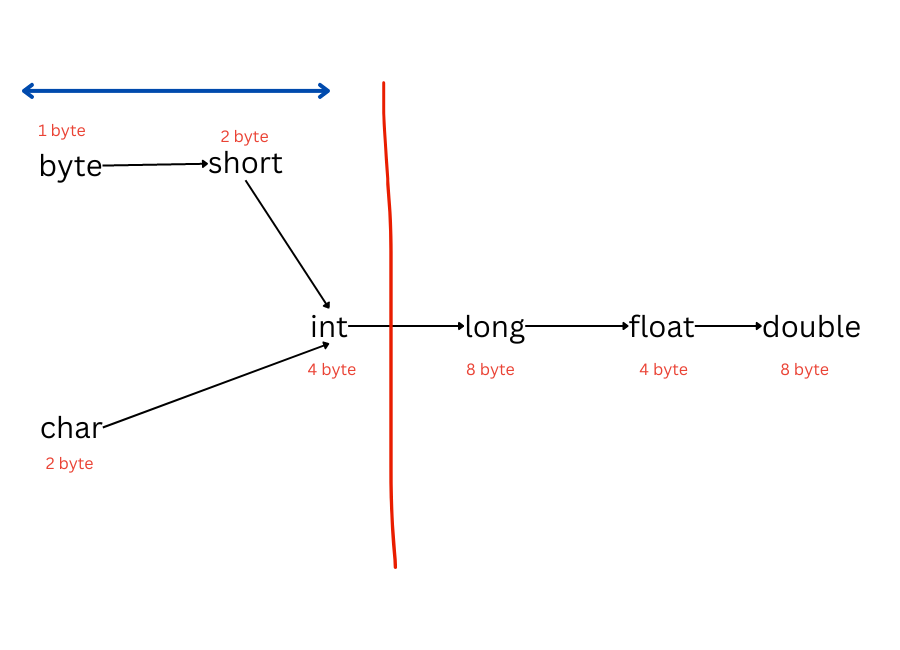
\includegraphics[scale=.4]{content/chapter4/images/allow.png}
	\end{figure}	
	Example:
	\codeblock{
		int[] x = new int[5]; \\
		x[0] = 10; \\
		x[1] = 'a'; \\
		byte b = 20; \\
		x[2] = b; \\
		short s = 30; \\
		x[3] = s; \\
		x[4] = 10L; \xmark
	}
	
	Similary, in case of float type arrays, the allowed datatypes are:
	\begin{itemize}
		\item byte
		\item short
		\item char
		\item int
		\item long
		\item float
	\end{itemize}
		
\end{flushleft}

\subsection{Array variable assignments}
\setlength{\columnsep}{3pt}
\begin{flushleft}
	\bigskip
	

	\begin{itemize}
		\item Data type level promotion are not applicable at array level.
		\item Eg: Char datatype can be promoted to int type. Whereas, char array cannot be promoted to int array.
		
		\codeblock{
			int[] x = \{10,20,30,40\}; \\
			char[] ch = \{'a','b','c','d'\}; \\
			int[] b = x; \cmark \\
			int[] c = ch; \xmark
		}
	\end{itemize}
	
	Which of the following promotions will be performed automatically:
	
	\begin{tabulary}{1.0\textwidth}{|p{12em}|p{12em}|}
		\toprule
		\textbf{Conversion} & \textbf{Answer} \\
		\midrule
		char $\rightarrow$ int & \cmark \\
		\hline
		char[] $\rightarrow$ int[] & \xmark \\
		\hline
		int $\rightarrow$ double & \cmark \\
		\hline
		int[] $\rightarrow$ double[] & \xmark \\
		\hline
		float $\rightarrow$ int & \xmark \\
		\hline
		float[] $\rightarrow$ int[] & \xmark \\
  		\bottomrule
	\end{tabulary}
	
\end{flushleft}

%-----------------------


%----------------------------------------------------------------------------------------
%	CHAPTER 3
%----------------------------------------------------------------------------------------
\chapterimage{index4.png} % Table of contents heading image
\chapter{Operators}
%-----------------------
\section{Operators in Java}
\setlength{\columnsep}{3pt}
\begin{flushleft}
	\bigskip
	\bigskip
	\begin{tcolorbox}[breakable,notitle,boxrule=1pt,colback=black,colframe=black]
		\color{white}
		\bigskip
		In this section, you are going to learn:
		\begin{enumerate}
			\item \textbf{Arithematic Operator}
			\item \textbf{String Concatenation Operator}
			\item \textbf{Increment/Decrement Operator}
			\item \textbf{Relational Operator}
			\item \textbf{Equality Operator}
			\item \textbf{Bitwise Operator}
			\item \textbf{Boolean complement Operator}
			\item \textbf{Short circuit Operator}
			\item \textbf{Type cast Operator}
			\item \textbf{Assignment Operator}
			\item \textbf{Conditional Operator}
			\item \textbf{new Operator}
			\item \textbf{ $\left[ \right]$ Operator}
			\item \textbf{Operator Precedence}
		\end{enumerate}	
	
	\end{tcolorbox}
	
\end{flushleft}

\newpage


\subsection{Arithematic Operator}
\setlength{\columnsep}{3pt}
\begin{flushleft}
	
	\tabletwo{
		\hline
		Operator &  Example \\
		\hline
		Addition(+) & 
		\bigskip
		\codecontinue{
			int a = 5; \\
			int b = 10; \\
			int c = a + b; // c will be 15 
			}  \\
		\hline
		
		Subtraction(-) & 
		\bigskip
		\codecontinue{
			int a = 10; \\
			int b = 5; \\
			int c = a - b; // c will be 5
		}  \\
		
		\hline
		
		Multiplication(*) & 
		\bigskip
		\codecontinue{
			int a = 2; \\
			int b = 3; \\
			int c = a * b; // c will be 6
		}  \\
		\hline
		
		Modulus (\%) &
		\bigskip
		\codecontinue{
			int a = 10;
			int b = 3;
			int c = a \% b; // c will be 1
		}
		\\
		
		\hline

	}
	
	\newpage
	
	\tabletwo{
		\hline
		Division(/) & 
		\bigskip
		\codecontinue{
			int a = 10; \\
			int b = 3; \\
			int c = a / b; // c will be 3 (the remainder is discarded) \\
			\\
			double d = 10.0; \\
			double e = 3.0; \\
			double f = d / e; // f will be 3.33333
		}  \\
		
		\hline
	}
	
	\textbf{Important Points:}
	\begin{itemize}
		\item \textbf{Implicit type casting:} If we apply any arithmetic operator between 2 variables “a” and “b”, the result type is always:
		\codecontinue{
			maximum(int, type of a, type of b)
		}
		
		Using above formula,
		\codecontinue{
			\begin{itemize}
				\item Byte + byte = int
				\item Byte + short = int
				\item Short + short = int
				\item Byte + long = long
				\item Long + double = double
				\item Float + long = float
				\item Char + char = int
				\item Char + double = double
			\end{itemize}
		}
		\newpage
		Eg:
		\codeblock{
			System.out.println('a'+'b'); // output: 195 \\
			System.out.println('a'+3.29); // output: 100.29
		}
	
		\bigskip
		
		\item \textbf{Infinity}: 
		\begin{itemize}
			\item In integral arithmetic \textbf{(byte short int long)}\textbf{, infinity cannot be represented} and JVM will return runtime error.
			\bigskip
			\codeblock{
				System.out.println(10/0); \xmark
			}
			
			\item But in \textbf{floating point arithmetic (float, double), infinity can be represented}.  For this, Float and Double classes contains below 2 constants:
			\begin{itemize}
				\item POSITIVE\_INFINITY;
				\item NEGATIVE\_INFINITY;
			\end{itemize}
			\bigskip		
			\codeblock{
				System.out.println(10/0.0); // output: Infinity\\
				System.out.println(-10/0.0); // output: -Infinity
			}
		\end{itemize}
		
		\bigskip
		\item \textbf{NaN (not a number):}
		\begin{itemize}
			\item In \textbf{integer arithmetic (byte, short, int, long) , undefined results cannot be represented} and JVM will return runtime error.
			\bigskip
			\codeblock{
			System.out.println(0/0);	\xmark				
			}
		
			\item But, in floating point arithmetic \textbf{(float,double), undefined results can be represented as NaN constant}.
			\bigskip
			\codeblock{
				System.out.println(0.0/0); // output: NaN \\
				System.out.println(-0/0.0); // output: NaN	
			}
				
		\end{itemize} 
		
	\end{itemize}
	
\end{flushleft}








\subsection{String Concatenation Operator}
\setlength{\columnsep}{3pt}
\begin{flushleft}
	
	\begin{itemize}
		\item The only overloaded operator in Java is \textbf{"+"} operator. 
		\item It can act as arithmetic addition operator as well as string concatecation operator.
		\bigskip
		\codeblock{
			System.out.println(10+20); // output: 30  \\
			System.out.println("ab"+"cd"); // output: abcd
		}
		\bigskip
		\noteblock{
			Apart from "+", Java does not support \textbf{operator overloading}!	
		}
	
		\item Working of \textbf{"+"} with string:
		
		\begin{itemize}
			\item If atleast one argument is string type, + operator acts as concatenation operator.
			\item If both arguments are number type, + operator acts as arithmetic addition operator.
		\end{itemize}
	
		Eg:
		\codeblock{
			String a = "lavatech";   \\
			int b=10, c=20, d=30;   		\\
			System.out.println(a+b+c+d);  // output: lavatech102030 \\
			System.out.println(b+c+d+a);  // output: 60lavatech		\\
			System.out.println(b+c+a+d);  // output: 30lavatech30		\\
			System.out.println(b+a+c+d);  // output: 10lavatech2030
		}
		
	\end{itemize}
	

\end{flushleft}

\newpage






\subsection{Increment/Decrement Operator}

\begin{flushleft}

	
	\begin{itemize}
		\item The increment(++) and decrement(--) operators are unary operators.
		\item They are used to increment or decrement the value of a variable by 1.
		\item \textbf{Increment Operator (++):} Used in two ways:
		\begin{itemize}
			\item \textbf{Prefix (++var)}: Variable is incremented first and then used in the expression.
			\bigskip
			\codeblock{
				int a = 5; \\
				int b = ++a; // b will be 6, a will be 6
			}
			
			\item \textbf{Postfix (var++)}: Variable is used in the expression and then incremented. 
			\bigskip
			\codeblock{
				int a = 5; \\
				int b = a++; // b will be 5, a will be 6
			}			
		\end{itemize}
		
		\item \textbf{Decrement Operator (--):} Works in a similar way and can be used in prefix and postfix forms:
		\bigskip
		\codeblock{
			int a = 5; \\
			int b = --a; // b will be 4, a will be 4  \\
			int c = a--; // c will be 4, a will be 3
		}
	\end{itemize}
	
	Summary:
	\tablefour{
		\hline
		Expression & Initial value of x & Value of y & Final value of x \\
		\hline
		y=++x; & 10 & 11 & 11 \\
		\hline
		y=++x; & 10 & 10 & 11 \\
		\hline
		y=++x; & 10 & 9 & 9 \\
		\hline
		y=++x; & 10 & 10 & 9 \\
		\hline
	}
	
	Important Points:
	\begin{itemize}
		\item Increment/decrement is \textbf{applicable only on variable and not on constant}.
		\bigskip
		\codeblock{
			System.out.println(++10); \xmark
		}
		\item \textbf{Listing} of increment/decrement operators \textbf{not allowed}.
		\bigskip
		\codeblock{
			int x=10; \\
			int y = ++(++x); \xmark
		}
	
		\item \textbf{For final variables}, increment/decrement operators \textbf{cannot} be used:
		\bigskip
		\codeblock{
			final int x=10; \\
			System.out.println(x++); \xmark
		}
	
		\item Increment/decrement is applicable on all primitive type, \textbf{except boolean datatype}:
		\begin{itemize}
			\item Integer example:
			\bigskip
			\codeblock{
				int x=10; \\
				x++; \\
				System.out.println(x);   // output: 11
			}
			\item Character example:
			\bigskip
			\codeblock{
				char ch = 'a'; \\
				ch++; \\
				System.out.println(ch); // output: 'b'
			}
			\newpage
			\item Boolean example:
			\bigskip
			\codeblock{
				boolean b=true;  \\
				b++;  \xmark  
			}
		
		
		\end{itemize}
		
	\end{itemize}
		
	\textbf{Difference between “x++” and “x=x+1”}
	
	\begin{itemize}
		\item We know that: If we apply any arithmetic operator between 2 variables “a” and “b”, the result type is always:
		\bigskip
		\codecontinue{
			maximum(int, type of a, type of b)
		}
		
		\item This is the reason why using "x=x+1" can result in compile-time error:
		\bigskip
		\codeblock{
			byte b=10; \\
			b = b+1;        \xmark 
		}
	
		\item But in case of increment/decrement operators, internal type casting will be performed automatically:
		\bigskip
		\codeblock{
			byte b=10;  \\
			b++;   \cmark
		}
		
	\end{itemize}
	
	
		
\end{flushleft}
\newpage
\subsection{Relational Operator}

\begin{flushleft}
	
	\begin{itemize}
		\item Below are available relational operator in Java:
		\newimage{0.5}{content/chapter3/images/relational.png}
		\item We can apply relational operator for every primitive datatype, except boolean datatype.
		\item Eg:
		\bigskip
		\codeblock{
			System.out.println(10>20);  // output: false  \\
			System.out.println('a'>20);  // output: false  \\ 
			System.out.println('b'>2.0); // output: false  \\
			//System.out.println(true > false); \xmark
		}
	
		\item We can’t apply relational operators for object types
		\bigskip
		\codeblock{
			System.out.println('lava' > 'lavatech');  \xmark
		}
	
		\item Chaining of relational operators is not allowed.
		\bigskip
		\codeblock{
			System.out.println(10>20>30);  \xmark
		}
		
	\end{itemize}
	
\end{flushleft}
\newpage
\subsection{Equality Operator}

\begin{flushleft}
	
	\begin{itemize}
		\item Equality operators can be used for every primitive type including boolean.
		\bigskip
		\codeblock{
			System.out.println(10==20);  // output: fasle \\
			System.out.println('a' == 'b'); // output: false \\
			System.out.println('a' == 97.0); // output: true \\
			System.out.println(false == false); // output: true
		}
		
		\item Equality operators can be applied for object types also. For object references, "r1" \& "r2", "r1==r2" returns true, if both reference pointing to the same object (reference comparison or address comparison)
		\bigskip
		\codeblock{
			Thread t1 = new Thread(); \\
			Thread t2 = new Thread(); \\
			Thread t3 = t1; \\
			System.out.println(t1 == t2);   // output: false \\
			System.out.println(t1 == t3);   // output: true
		}
		
		There should be some relation between argument types(either child to parent or parent to child or same type). Otherwise, it will result in compile-time error.
		\bigskip
		\codeblock{
			Thread t1 = new Thread();   \\
			Object o = new Object();   \\
			String s = new String("lava");   \\
			System.out.println(t1==o) ; // output: false    \\
			System.out.println(o==s); // output: false    \\
			//System.out.println(s==t1); \xmark
		}
		
		For any object reference "r": "r==null"  ← is always False
		\bigskip
		\codeblock{
			String s1 = new String("lava"); \\
			System.out.println(s1 == null) ; // output: false \\
			\\
			String s2 = new String(); \\
			System.out.println(s2==null); // output: false \\
			\\
			String s3 = null; \\
			System.out.println(s3==null); // output: true
		}
		
	\end{itemize}


	
\end{flushleft}
\newpage
\subsection{Bitwise Operator}

\begin{flushleft}

	\bigskip
	\begin{figure}[h!]
		\centering
		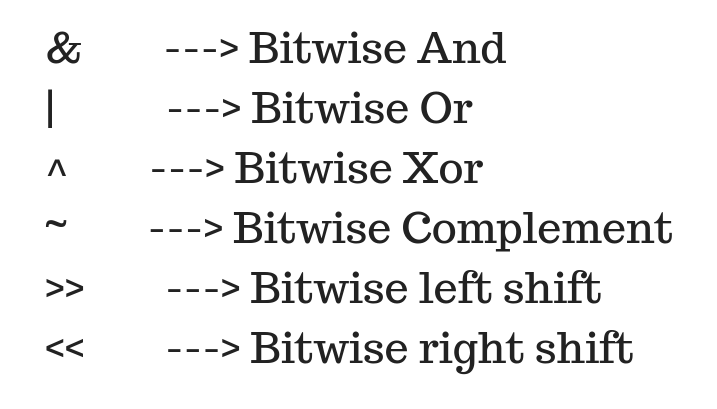
\includegraphics[scale=0.5]{content/chapter3/images/bitwise2.png}
	\end{figure}
	
	\begin{tabular}{|p{10em}|p{8em}|p{6em}|}
		
		\multicolumn{3}{l}{} \\
		\multicolumn{3}{l}{\textbf{Bitwise \&} - If both bits are 1, then only 1 otherwise 0}                  
		\\ \hline
		\multicolumn{1}{|l|}{Sample Code} & \multicolumn{1}{l|}{Output}  & \multicolumn{1}{l|}{Explaination}   
		\\ \hline
		\multicolumn{1}{|l|}{\begin{tabular}[c]{@{}l@{}}int a=4; \\
				int b=5; \\
				System.out.println(a \& b)	 \end{tabular}}  & 
		\multicolumn{1}{l|}{4}   &  
		\multicolumn{1}{|l|}{\begin{tabular}[c]{@{}l@{}}100 \\
				101 \\
				----- \\
				100	 \end{tabular}}  
		\\ 
		\hline
	
		\multicolumn{3}{l}{} \\
		\multicolumn{3}{l}{\textbf{Bitwise |} - If atleast one bit is 1, then only 1 otherwise 0}                  
		\\ \hline
		\multicolumn{1}{|l|}{Sample Code} & \multicolumn{1}{l|}{Output}  & \multicolumn{1}{l|}{Explaination}   
		\\ \hline
		\multicolumn{1}{|l|}{\begin{tabular}[c]{@{}l@{}}int a=4; \\
				int b=5; \\
				System.out.println(a | b)	 \end{tabular}}  & 
		\multicolumn{1}{l|}{5}   &  
		\multicolumn{1}{|l|}{\begin{tabular}[c]{@{}l@{}}100 \\
				101 \\
				----- \\
				101	 \end{tabular}}  
		\\ 
		\hline
	
		
	\end{tabular}
	
	\newpage
	
	\begin{tabular}{|p{10em}|p{8em}|p{8em}|}
		
		\multicolumn{3}{l}{} \\
		\multicolumn{3}{l}{\textbf{Bitwise \^} - Also called x-or. If both bits are different, then 1, otherwise 0}                  
		\\ \hline
		\multicolumn{1}{|l|}{Sample Code} & \multicolumn{1}{l|}{Output}  & \multicolumn{1}{l|}{Explaination}   
		\\ \hline
		\multicolumn{1}{|l|}{\begin{tabular}[c]{@{}l@{}}int a=4; \\
				int b=5; \\
				System.out.println(a \textbf{\^} b)	 \end{tabular}}  & 
		\multicolumn{1}{l|}{1}   &  
		\multicolumn{1}{|l|}{\begin{tabular}[c]{@{}l@{}}100 \\
				101 \\
				----- \\
				001	 \end{tabular}}  
		\\ 
		\hline
		
		\multicolumn{3}{l}{} \\
		\multicolumn{3}{l}{\textbf{Bitwise \~} - Bitwise complement operator, 1 becomes 0 and 0
becomes 1}                  
		\\ \hline
		\multicolumn{1}{|l|}{Sample Code} & \multicolumn{1}{l|}{Output}  & \multicolumn{1}{l|}{Explaination}   
		\\ \hline
		\multicolumn{1}{|l|}{\begin{tabular}[c]{@{}l@{}}int a=4; \\
				System.out.println( \textbf{\~} a)	 \end{tabular}}  & 
		\multicolumn{1}{l|}{-5}   &  
		\multicolumn{1}{|l|}{\begin{tabular}[c]{@{}l@{}} 32-bit os represents number with	\\
				total 32 bits as 000...000100 \\
				 \textbf{\~} 000...000100 = 111...111011 \\
				Left most bit is sign bit where, \\
				1 is negative and 0 is positive \\
				Since left most bit is now 1, number is negative \\
				Negative number is represented as \\
				1's complement + 1 \\
				ie. 100..000100 + 1 = 100...000101	
		 \end{tabular}}  
		\\ 
		\hline
	

		\multicolumn{3}{l}{} \\
		\multicolumn{3}{l}{\begin{tabular}[c]{@{}l@{}}\textbf{Bitwise >>} - Bitwise right shift. \\
		Remove "x" bit from right side and add "x" 0 to left side.	 \end{tabular}}                  
		\\ \hline
		\multicolumn{1}{|l|}{Sample Code} & \multicolumn{1}{l|}{Output}  & \multicolumn{1}{l|}{Explaination}   
		\\ \hline
		\multicolumn{1}{|l|}{\begin{tabular}[c]{@{}l@{}}int a=10; \\
				int x=2; \\
				System.out.println(a >> x)	 \end{tabular}}  & 
		\multicolumn{1}{l|}{2}   &  
		\multicolumn{1}{|l|}{\begin{tabular}[c]{@{}l@{}}000...1010 >> 2 \\
				000...0010 \\
					 \end{tabular}}  
		\\ 
		\hline
	\end{tabular}

	\newpage
	
	\begin{tabular}{|p{10em}|p{8em}|p{6em}|}
		
		
	\multicolumn{3}{l}{} \\
	\multicolumn{3}{l}{\begin{tabular}[c]{@{}l@{}}\textbf{Bitwise <<} - Bitwise left shift. \\	
	Remove "x" bit from left side and add "x" 0 to right side.	 \end{tabular}}                  
	\\ \hline
	\multicolumn{1}{|l|}{Sample Code} & \multicolumn{1}{l|}{Output}  & \multicolumn{1}{l|}{Explaination}   
	\\ \hline
	\multicolumn{1}{|l|}{\begin{tabular}[c]{@{}l@{}}int a=10; \\
			int x=2; \\
			System.out.println(a << x)	 \end{tabular}}  & 
	\multicolumn{1}{l|}{40}   &  
	\multicolumn{1}{|l|}{\begin{tabular}[c]{@{}l@{}}000...1010 << 2 \\
			000...101000 \\
	\end{tabular}}  
	\\ 
	\hline
		
	\end{tabular}
		
	\noteblock{
		\begin{itemize}
			\item \&, | , \textbf{\^}  are applicable for both boolean and integral type.
			\item >> , << are applicable for integral type only.
			\item \textbf{\~} applicable for only integral type but not for boolean type.
		\end{itemize}	
	}
		
		
\end{flushleft}

\subsection{Boolean complement operator}

\begin{flushleft}
	
	\begin{itemize}
		\item The Boolean complement operator (!) is a unary operator that negates the value of a Boolean expression. 
		\bigskip
		\codeblock{
			boolean a = true; \\
			boolean b = !a; // output: b is false 
		}
		\bigskip
		\noteblock{
			! operator can be applied only on boolean data-type.
		}
		
	\end{itemize}
	
\end{flushleft}
\newpage
\subsection{Short circuit Operator}

\begin{flushleft}
	
	 	In Java, the short-circuit operators are:
		\begin{itemize}
			\item \textbf{\&\& (logical AND)}: Same as bitwise \&
			\item \textbf{|| (logical OR)}: Same as bitwise |
		\end{itemize}

		\tabletwo{
		\hline
		\& , |  & \&\& , || \\
		\hline
		Both arguments should be evaluated always & Second argument evaluation is optional \\
		\hline
		Relatively performance is low & Relatively performance is high \\
		\hline
		Applicable for both boolean and integral types & Applicable only for boolean but not for integral types \\
		\hline
		Eg: \newline
		For x \& y, both x and y will be evaluated. \newline
		Similarly, \newline
		For x | y, both x and y will be evaluated. 
		& 
		Eg: \newline
		For x \&\& y, y will be evaluated if and only if x is true i.e if x is false then y wont be evaluated. \newline
		Similarly, \newline
		For x || y,  y will be evaluated if and only if x is false i.e if x is true then y wont be evaluated. \\
		
		\hline
		
		}
		
		\bigskip
		Consider below code showing different behaviour of \&, \&\&, |, ||:
		\codeblock{
			int x = 10, y = 15;   \\
			if(  ++x < 10  \& ++y > 15) \{ \\
			\s	x++;   \\
			\}  \\
			else \{  \\
			\s	y++;   \\
			\}  \\
			System.out.println(x + "..." + y);  //   output: 11...17
		}
		\bigskip
		\codeblock{
			int x = 10, y = 15;   \\
			if(  ++x < 10  | ++y > 15) \{ \\
			\s	x++;   \\
			\}  \\
			else \{  \\
			\s	y++;   \\
			\}  \\
			System.out.println(x + "..." + y);  //   output: 12...16
		}
		\bigskip
		\codeblock{
			int x = 10, y = 15;   \\
			if(  ++x < 10  \&\& ++y > 15) \{ \\
			\s	x++;   \\
			\}  \\
			else \{  \\
			\s	y++;   \\
			\}  \\
			System.out.println(x + "..." + y);  //   output: 11...16
		}
		\bigskip
				\codeblock{
			int x = 10, y = 15;   \\
			if(  ++x < 10  || ++y > 15) \{ \\
			\s	x++;   \\
			\}  \\
			else \{  \\
			\s	y++;   \\
			\}  \\
			System.out.println(x + "..." + y);  //   output: 12...16
		}
		\bigskip

	
\end{flushleft}
\newpage
\subsection{Assignment Operator}

\begin{flushleft}
	
	There are 3 types of assignment operators:
	\begin{itemize}
		\item \textbf{Simple:}  The assignment operator (=) is used to assign a value to a variable.
		\bigskip
		\codeblock{
			int x = 10;
		}
		\item \textbf{Chained:} 
		\bigskip
		\codeblock{
			int a,b,c,d; \\
			a=b=c=d=20;   
		}
	
		We can’t perform chained assignment directly at the time of declaration:
		\bigskip
		\codeblock{
			int a=b=c=d=20; \xmark \\
						\\
			int b,c,d;  \\
			int a=b=c=d=20;  \cmark
		}
		
		\item \textbf{Compound:} 
		\begin{itemize}
			\item Assignment operator can be mixed with other operators.
			\item Such type of assignment operators are called compound assignment operators.
			\bigskip
			\syntaxblock{
				variable operator= expression;
			}
			\bigskip
			\codeblock{
				int a = 10;  \\
				a += 20;  \\
				System.out.println(a) ; // output: 30
			}
			
			\item In case of compound assignment operator, internal type casting will be performed automatically:
			\bigskip
			\codeblock{
				byte b=10;  \\
				b = b+1;     \xmark \\
				\\
				byte b = 10; \\
				b++;    // output: 11 \\    
				\\
				byte b=10; \\
				b+=1;    // output: 11
			}
			\bigskip
			\item Below are sample examples of compound assignment operator:
			\codeblock{
				int x = 5;
				x += 3; // x is 8 \\
				x -= 2; // x is 6 \\
				x *= 4; // x is 24 \\
				x /= 3; // x is 8  \\
				x \%= 5; // x is 3  \\
				x \&= 1; // x is 1 \\
				x |= 2; // x is 3 \\
				x \textbf{\^}= 3; // x is 0 \\
				x <<= 2; // x is 0 \\
				x >>= 1; // x is 0
			}
		\end{itemize}
		 
		
		
		
	\end{itemize}
	
	
	
	
\end{flushleft}
\newpage
\subsection{Conditional Operator}

\begin{flushleft}
	
	\begin{itemize}
		\item The conditional operator (also known as the ternary operator)
		\item It is \textbf{if-else statement in a single line}. 
		\bigskip
		\syntaxblock{
			condition ? expression1 : expression2	
		}
		
		\item If condition is true, then the expression1 is evaluated else expression2 is evaluated and its value is returned.
		\bigskip
		\codeblock{
			int a = 23, b = 30; \\
			System.out.println( (a>b)? "a is greater" : "b is greater");
		}
		
	\end{itemize}
	
	
	
	
\end{flushleft}

%\subsection{instanceOf Operator}
%\setlength{\columnsep}{3pt}
\begin{flushleft}
	\bigskip
	\begin{figure}[h!]
		\centering
		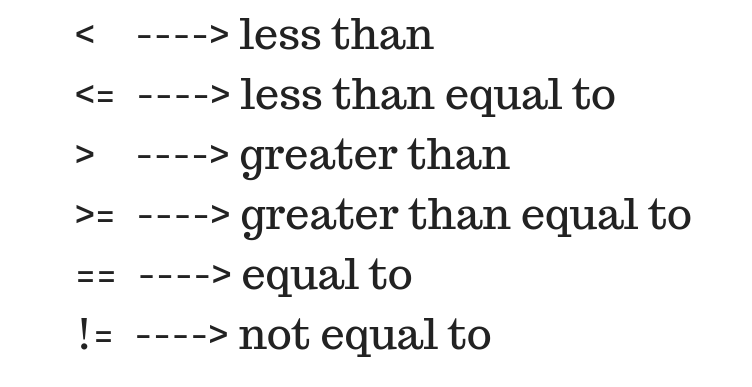
\includegraphics[scale=0.5]{content/chapter3/images/relational.png}
	\end{figure}

	\begin{tcolorbox}[breakable,notitle,boxrule=1pt,colback=yellow,colframe=yellow]
		\color{black}
		\fontdimen2\font=8pt
		\textbf{Note}: 
		\begin{itemize}
			\item \textbf{"<" , "<=" , ">" , ">="} are applicable on integers, strings \& boolean , but not on cross datatypes.	
			\item \textbf{"==" , "!="} are applicable on all datatypes, including cross datatypes.
			\item \textbf{"==" , "!="} never returns error.
		\end{itemize}
		\fontdimen2\font=4pt
	\end{tcolorbox}
	
	\newpage

	Sample code 1:
	\begin{tcolorbox}[breakable,notitle,boxrule=-0pt,colback=code,colframe=code]
			\color{white}
			\fontdimen2\font=8pt
			a=6 \newline
			b=2 \newline
			print(a>b, a<b) \newline
			a=6 \newline
			b=6 \newline
			print(a>=b, a<=b) \newline
			a="apple" \newline
			b="mango" \newline
			print(a>b, a<b)
			\fontdimen2\font=4pt
	\end{tcolorbox}
		
	Output:
	\begin{tcolorbox}[breakable,notitle,boxrule=-0pt,colback=output,colframe=output]
			\color{black}
			True False \newline
			True True \newline
			False True
			\fontdimen2\font=4pt
	\end{tcolorbox}
	\bigskip \bigskip
	Sample code 2:
		\begin{tcolorbox}[breakable,notitle,boxrule=-0pt,colback=code,colframe=code]
		\color{white}
		\fontdimen2\font=8pt
		a=6 \newline
		b="6" \newline
		print(a==b, a!=b) \newline
		a=6 \newline
		b=6 \newline
		print(a==b, a!=b)
		\fontdimen2\font=4pt
	\end{tcolorbox}
	
	Output:
	\begin{tcolorbox}[breakable,notitle,boxrule=-0pt,colback=output,colframe=output]
		\color{black}
		False True \newline
		True False
		\fontdimen2\font=4pt
	\end{tcolorbox}
\end{flushleft}

\newpage






\subsection{new Operator}

\begin{flushleft}
	
	\begin{itemize}
		\item \textbf{new} operator is used to create an object.
		
		\bigskip
		\syntaxblock{
			Class obj = new class();
		}
		
		Eg:
		\codeblock{
			String name = new String("Ram");
		}
		
	\end{itemize}
	
\end{flushleft}

\subsection{ $\left[ \s \right]$ Operator}

\begin{flushleft}
	
	\begin{itemize}
		\item $\left[ \s \right]$ operator is used to declare and create arrays.
		
		\bigskip
		\codeblock{
			int[] x = new int[10]; 
		}
			
	\end{itemize}
	
\end{flushleft}

\subsection{Operator Precedence}

\begin{flushleft}
	
	\tabletwo{
	\hline
	Unary operators &  [] , x++ , x-- \newline ++x , --x , \textbf{\~} , ! \\
	\hline
	Arithematic operators &  * , / , \%  \newline + , - \\
	\hline
	Shift operators & >>  , >>> , << \\
	\hline
	Comparison operators & < , <= , > , >= , instanceof \\
	\hline
	Equality operators &  == , != \\
	\hline
	Bitwise operators & \& , \textbf{\^} , | \\
	\hline
	Short circuit operators & \&\& , || \\
	\hline
	Conditional operator & ?: \\
	\hline
	Assignment operators &  = , += , -= , *= \\
	\hline
	}

	\textbf{Evaluation order of operands:}
	
	\begin{itemize}
		\item In java, we have only operator precedence and no operands precedence.
		\item Before applying any operator, all operands will be evaluated from left to right.
		\item Eg:
		\codeblock{
			System.out.println(1+2*3/4+5*6);  // output: 32
		}
	
		Output explaination:
		\begin{itemize}
			\item 1+2*3/4+5*6
			\item 1+6/4+5*6
			\item 1+1+5*6
			\item 1+1+30
			\item 32
		\end{itemize}
		
	\end{itemize}
	
\end{flushleft}

%-----------------------

%----------------------------------------------------------------------------------------
%	CHAPTER 6
%----------------------------------------------------------------------------------------
\chapterimage{index4.png} % Table of contents heading image
\chapter{Flow Control}
%-----------------------
\section{Flow control statement}
\setlength{\columnsep}{3pt}
\begin{flushleft}
	\bigskip
	\bigskip
	In this section, you are going to learn:	\newimage{0.68}{content/chapter4/images/loop.png}
	
	
	
\end{flushleft}

\newpage


\section{Selection Statements}
\setlength{\columnsep}{3pt}
\begin{flushleft}
	
	Below are 2 selection statements:
	\begin{itemize}
		\item \textbf{if..else}
		\item \textbf{switch case}
	\end{itemize}
	Let's see each of these in detail.
	
	
\end{flushleft}






\subsection{if...else}
\setlength{\columnsep}{3pt}
\begin{flushleft}
	
	\begin{itemize}
		\item The \textbf{if} statement allows you to execute a block of code if a certain condition is true.
		\bigskip
		\syntaxblock{
			if (condition) \\
			\s Action if is true
		}		
		\bigskip
		\syntaxblock{
			if (condition) \{ \\
			\s Action if is true \\
			\} \\
			else \{ \\
			\s Action if is false \\
			\} 
		}
		
		
		\item The argument to if statement should be boolean type only, else there will be compile-time error.
		
		\item \textbf{Else part and curly braces are optional.}
		\item Without curly braces only one statement is allowed under if statement, which should \textbf{not be declarative statement}.
		\newpage
		\item Eg 1:
		\codeblock{
			if (true) \\
			\s System.out.println("Hello");
		}
		
		\item Eg 2:
		\codeblock{
			if (true);		\cmark // Note: Semicolon is also valid statement.
			
		}
		
		\item Eg 3:
		\codeblock{
			if (true) \\
			\s int x = 10;  \xmark // Compile-time error for declarative statement
		}
		
		\item Eg 4:
		\codeblock{
			if (true) \{ \\
			\s	int x = 10; \\ 
			\}
		}
		
		\item Eg 5:
		\codeblock{
			int x = 0; \\
			if (x) \{          \xmark // Compile-time error as not a boolean     \\
			\s System.out.println("Hello"); \\
			\} \\
			else \{ \\
			\s System.out.println("Hi"); \\
			\} 
		}
		\newpage
		\item Eg 6:
		\codeblock{
			int x = 0; \\
			if (x=20) \{          \xmark // Compile-time error as not a boolean     \\
			\s System.out.println("Hello"); \\
			\} \\
			else \{ \\
			\s System.out.println("Hi"); \\
			\} 
		}
		
		\item Eg 7:
		\codeblock{
			int x = 0; \\
			if (x==20) \{   \\
			\s System.out.println("Hello"); \\
			\} \\
			else \{ \\
			\s System.out.println("Hi"); // output: Hi \\
			\} 
		}
		
		\item Eg 8:
		\codeblock{
			boolean b = false; \\
			if (b == false) \{   \\
			\s System.out.println("Hello"); // output: Hello \\
			\} \\
			else \{ \\
			\s System.out.println("Hi");  \\
			\} 
		}
	\end{itemize}
	
	\newpage
	
	\textbf{Dangling else}
	
	\begin{itemize}
		\item There is no dangling else problem in Java.
		\item Every else is mapped to the nearest if statement.
		
		\codeblock{
			if (true)  \\
			if (true) \\
			\s System.out.println("Hello"); // output: Hello \\
			else \\
			\s System.out.println("Hi");  \\
		}	
	\end{itemize}
	
	
	
	
	
	
\end{flushleft}

\newpage






\subsection{switch case}
\setlength{\columnsep}{3pt}
\begin{flushleft}
	
	\begin{itemize}
		\item If several options ar available, then it is not recommended to use nested if..else statement, as it reduces readability.
		
		\item Solution: switch statement
		\bigskip
		\syntaxblock{
			switch(argument) \{ \\
			\s	case arg-1:  	\\
			\s \s	action1;	\\
			\s \s	break;		\\
			\s	case arg-2:		\\
			\s \s	action2;		\\
			\s \s	break;		\\
			\s	case n:		\\
			\s \s	action-n;	\\
			\s \s	break		\\
			\s	default:		\\
			\s \s	Default action	\\
			\}
		}
		\bigskip
		\item Curly braces are mandatory.
		\item \textbf{Case and default are optional}, i.e an empty switch statement is a valid Java syntax.
		\codeblock{
			int x = 10; \\
			switch(x) \{\}  \cmark
		}
		\bigskip
		\item Allowed argument types in switch statement:
		\begin{itemize}
			\item Upto Java 1.4 version -> \textbf{byte, short, char, int}
			\item From Java 1.5 version -> byte, short, char, int, \textbf{wrapper classes (Byte, Short, Character, Integer), enum}
			\item From Java 1.7 versionbyte, short, char, int, wrapper classes (Byte, Short, Character, Integer), enum, \textbf{string}
		\end{itemize}
		
		\bigskip	
		\item Inside switch, every statement should be under some case or default.
		
		\codeblock{
			int x = 10; \\
			switch(x)\{   \\
			\s System.out.println();   \xmark \s // Compile-time error! \\
			\}
		}
		
		\item Case argument should be compile-time constant (i.e constant expression).
		\bigskip
		\codeblock{
			int x=10; \\
			int y=20; \\
			switch(x) \{ \\
			\s case 10:  \\
			\s \s System.out.println(10); \\
			\s \s	break; \\
			\s case y;    \xmark \s // Compile-time error!   \\         
			\s \s System.out.println(); \\
			\s \s	break; \\
			\} 
		}
		\bigskip
		\noteblock{
			If y is declared as "final", then there will be no compile-time error.
		}
		
		\newpage
		
		\item Switch arguments and case label can be expressions. But, case label should be constant expression.
		
		\codeblock{
			int x = 10; \\
			switch(x+1) \{ \\
			\s case 10: \\
			\s \s System.out.println(10); \\
			\s \s break; \\
			\s case 10+20+30: \\
			\s \s System.out.println(60); \\
			\s \s break; \\
			\}
		}
		\bigskip
		\item \textbf{Case label should be in range of switch arg type}, else it will result in compile-time error.
		\newline
		Eg 1:
		\codeblock{
			byte b = 10; \\
			switch(b) \{ \\			
			\s case 10: \\
			\s \s System.out.println(10); \\
			\s \s break; \\
			\s case 100: \\
			\s \s System.out.println(100); \\
			\s \s break; \\
			\s case 1000:   \xmark \s // Compille-time error! \\
			\s \s System.out.println(1000); \\
			\s \s break; \\				
			\}
		}
		\newpage
		
		Eg 2:
		\codeblock{
			byte b = 10; \\
			switch(b+1) \{  // Implicit type-caste to integer \\			 
			\s case 10: \\
			\s \s System.out.println(10); \\
			\s \s break; \\
			\s case 100: \\
			\s \s System.out.println(100); \\
			\s \s break; \\
			\s case 1000:  \\
			\s \s System.out.println(1000); \\
			\s \s break; \\				
			\}
		}
		
		\item Duplicate case labels are not allowed.
		\bigskip
		
		\codeblock{
			int x = 10; \\
			switch(x) \{  \\			 
			\s case 12: \\
			\s \s System.out.println(12); \\
			\s \s break; \\
			\s case 97: \\
			\s \s System.out.println(97); \\
			\s \s break; \\
			\s case 'a':   \xmark \s // Duplicate labels error    \\
			\s \s System.out.println(1000); \\
			\s \s break; \\				
			\}
		}
	\end{itemize}
	
	\newpage
	\textbf{Summary for case-label argument}
	\begin{itemize}
		\item It should  be constant expression.
		\item The value should be in the range of switch argument type.
		\item Duplicate case label are not allowed
	\end{itemize}
	
	\bigskip
	\bigskip
	\bigskip
	\textbf{Fall-through inside switch}
	\begin{itemize}
		\item Within the switch, if any case is matched, from that case onwards all statements will be executed until break or end of the switch.
		\item This is called fall-through inside switch.
		\item The main advantage of fall inside the switch is, we can define common action for multiple cases (code-reuseablilty).
		\bigskip
		\syntaxblock{
			switch(argument) \{  \\
			\s	case arg-1: \\
			\s	case arg-2: \\
			\s	case arg-3: \\
			\s \s		action; \\
			\s \s		break; \\
			\s	case arg-4: \\
			\s	case arg-5: \\
			\s	case arg-6: \\
			\s \s		action; \\
			\s \s		break; \\
			\}
		}
		\newpage
		Eg:
		\codeblock{
			int x = 0;
			switch(x) \{ \\
			\s case 0: \\
			\s \s System.out.println(0); \\
			\s case 1: \\
			\s \s System.out.println(1); \\
			\s \s break; \\
			\s case 2: \\
			\s \s System.out.println(2); \\
			\s default: \\
			\s \s System.out.print("default"); \\
			\}
		}
		\bigskip
		\outputblock{
			0 \\
			1
		}
		\item \textbf{Default case:}
		\begin{itemize}
			\item Within the switch, \textbf{you can take default case at most once}.
			\item Default case will be executed if and only if, there is no case matched.
			\item Within the switch, you can write default case anywhere but it is recommended to write as last case. \newline
			Eg:
			\codeblock{
				int x = 3;
				switch(x) \{ \\
				\s	default:  \\
				\s \s	System.out.println("default") \\
				\s case 0:  \\
				\s \s 	System.out.println(0) \\
				\s case 1: 
			}
			\newpage
			\codecontinue{
				\s \s	System.out.println(1) \\
				\s case 2: \\
				\s \s	System.out.println(2) \\
				\}
			}
			\bigskip
			\outputblock{
				default \\
				0
			}
		\end{itemize}
	\end{itemize}
	
	
\end{flushleft}

\newpage






\section{Iteration}
\setlength{\columnsep}{3pt}
\begin{flushleft}
	
	Iterative statements allow you to repeat a block of code multiple times. 
	\newline
	Below are the important iterative statements in Java:
	\begin{enumerate}
		\item while
		\item do-while
		\item for
		\item for-each
	\end{enumerate}
	
	
\end{flushleft}



\subsection{while()}
\setlength{\columnsep}{3pt}
\begin{flushleft}
	
	
	\begin{itemize}
		\item When number of iterations is not known in advance, you should use while loop.
		\bigskip
		\syntaxblock{
			while(condition) \{ \\
			\s	Action \\
			\}	
		}
		
		\item The condition should be of boolean type.
		\noteblock{
			In Java, "1" is not true or false.
			\codeblock{
				while(1) \{  \xmark  \\  
				\s	System.out.println("Hello"); \\
				\}
			}
		}
		
		\item Curly braces are optional and without curly you can take only one statement under while, and this statement \textbf{should not be declarative}.
		
		\item Below are some valid and invalid examples of while:
		\bigskip
		\codeblock{
			while(true) \cmark \\ 
			\s	System.out.println("Hello"); 
		}
		\bigskip
		\codeblock{
			while(true); \cmark
		}
		\bigskip
		\codeblock{
			while(true) \\
			\s int x = 10; \xmark
		}
		\bigskip
		\codeblock{
			while(true) \{ \\
			\s int int x = 10; \cmark \\
			\}
		}
		\item Unreachable statement in while loop also results in compile-time error. Below are some examples showing unreachable statement:
		\bigskip
		\codeblock{
			while(true) \{ \\
			\s	System.out.println("Hello");  \\
			\} \\
			System.out.println("Hi");   \xmark // Compile-time error 
		}
				
	\end{itemize}
	
\end{flushleft}
\newpage

\subsection{do-while()}
\setlength{\columnsep}{3pt}
\begin{flushleft}
	
	\begin{itemize}
		\item The partition table in MBR can hold only \textbf{4 entries}.
		\item Hence, there can be only \textbf{four partitions in hard disks}.
		\item These 4 partitions are called primary partitions.
		\item OS can be installed on the primary partition.
		\begin{figure}[h!]
			\centering
			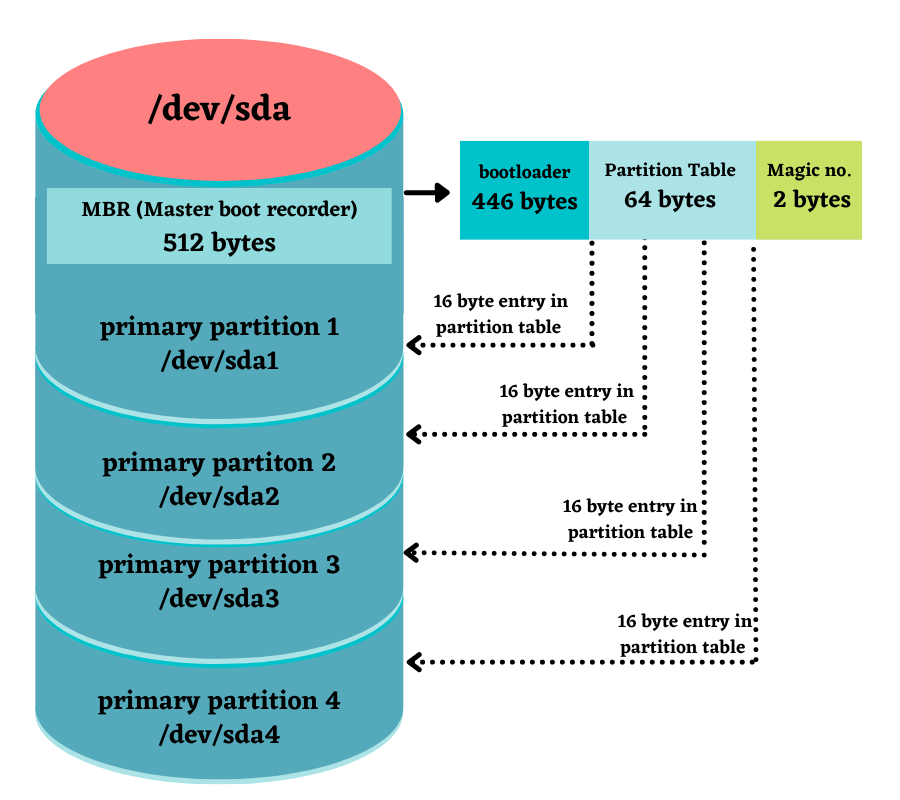
\includegraphics[scale=.6]{content/chapter8/images/correct.png}
			\caption{Primary partitions}
			\label{primary_naming}
		\end{figure}		
		
	\end{itemize}

\newpage

\paragraph{Command to create primary partition}

\bigskip
\textbf{fdisk}: Used to change the partition table.
	\bigskip
	\begin{tcolorbox}[breakable,notitle,boxrule=-0pt,colback=pink,colframe=pink]
		\color{black}
		\fontdimen2\font=9pt
		Syntax: fdisk device\_name
		\fontdimen2\font=4pt
	\end{tcolorbox}

	Options for \textbf{fdisk} command:
	\begin{itemize}
		\item \textbf{p}: Print the partition table
		\item \textbf{n}: Create a new partition
		\item \textbf{w}: Write the new partition table and exit
	\end{itemize}

	Eg:
	\begin{figure}[h!]
		\centering
		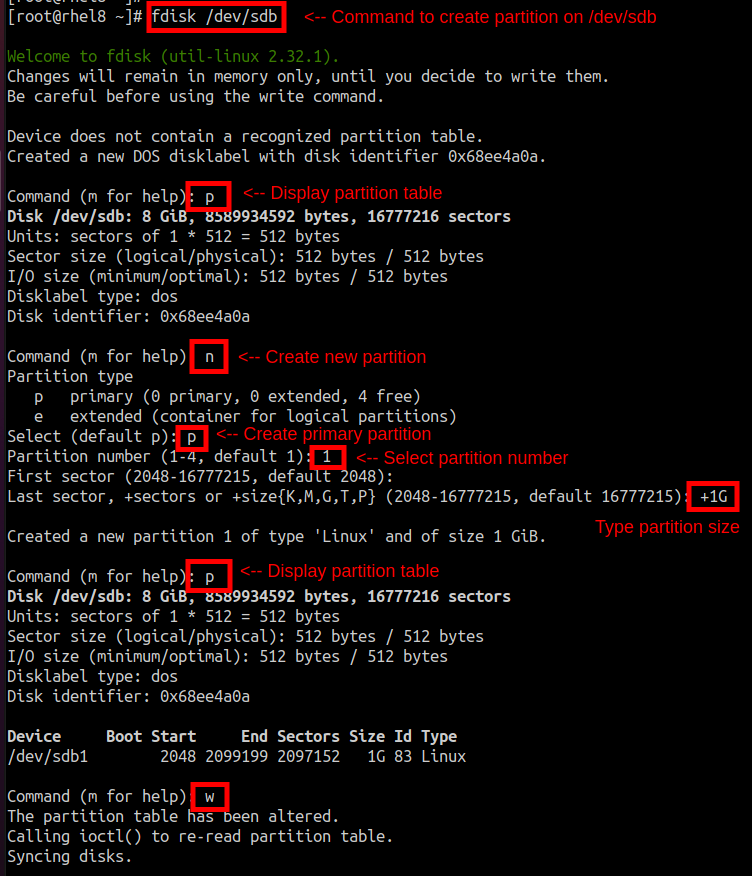
\includegraphics[scale=.4]{content/chapter8/images/primary_fdisk.png}
		\caption{Creating primary partitions}
		\label{pp}
	\end{figure}		
			
	
\end{flushleft}

\newpage


\subsection{for()}

\begin{flushleft}
	
	\begin{itemize}
		\item Equality operators can be used for every primitive type including boolean.
		\bigskip
		\codeblock{
			System.out.println(10==20);  // output: fasle \\
			System.out.println('a' == 'b'); // output: false \\
			System.out.println('a' == 97.0); // output: true \\
			System.out.println(false == false); // output: true
		}
		
		\item Equality operators can be applied for object types also. For object references, "r1" \& "r2", "r1==r2" returns true, if both reference pointing to the same object (reference comparison or address comparison)
		\bigskip
		\codeblock{
			Thread t1 = new Thread(); \\
			Thread t2 = new Thread(); \\
			Thread t3 = t1; \\
			System.out.println(t1 == t2);   // output: false \\
			System.out.println(t1 == t3);   // output: true
		}
		
		There should be some relation between argument types(either child to parent or parent to child or same type). Otherwise, it will result in compile-time error.
		\bigskip
		\codeblock{
			Thread t1 = new Thread();   \\
			Object o = new Object();   \\
			String s = new String("lava");   \\
			System.out.println(t1==o) ; // output: false    \\
			System.out.println(o==s); // output: false    \\
			//System.out.println(s==t1); \xmark
		}
		
		For any object reference "r": "r==null"  ← is always False
		\bigskip
		\codeblock{
			String s1 = new String("lava"); \\
			System.out.println(s1 == null) ; // output: false \\
			\\
			String s2 = new String(); \\
			System.out.println(s2==null); // output: false \\
			\\
			String s3 = null; \\
			System.out.println(s3==null); // output: true
		}
		
	\end{itemize}


	
\end{flushleft}
\newpage
\subsection{for-each loop}

\begin{flushleft}

	\bigskip
	\begin{figure}[h!]
		\centering
		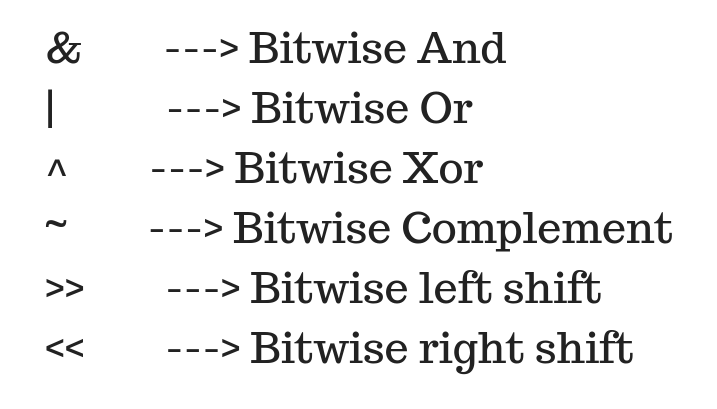
\includegraphics[scale=0.5]{content/chapter3/images/bitwise2.png}
	\end{figure}
	
	\begin{tabular}{|p{10em}|p{8em}|p{6em}|}
		
		\multicolumn{3}{l}{} \\
		\multicolumn{3}{l}{\textbf{Bitwise \&} - If both bits are 1, then only 1 otherwise 0}                  
		\\ \hline
		\multicolumn{1}{|l|}{Sample Code} & \multicolumn{1}{l|}{Output}  & \multicolumn{1}{l|}{Explaination}   
		\\ \hline
		\multicolumn{1}{|l|}{\begin{tabular}[c]{@{}l@{}}int a=4; \\
				int b=5; \\
				System.out.println(a \& b)	 \end{tabular}}  & 
		\multicolumn{1}{l|}{4}   &  
		\multicolumn{1}{|l|}{\begin{tabular}[c]{@{}l@{}}100 \\
				101 \\
				----- \\
				100	 \end{tabular}}  
		\\ 
		\hline
	
		\multicolumn{3}{l}{} \\
		\multicolumn{3}{l}{\textbf{Bitwise |} - If atleast one bit is 1, then only 1 otherwise 0}                  
		\\ \hline
		\multicolumn{1}{|l|}{Sample Code} & \multicolumn{1}{l|}{Output}  & \multicolumn{1}{l|}{Explaination}   
		\\ \hline
		\multicolumn{1}{|l|}{\begin{tabular}[c]{@{}l@{}}int a=4; \\
				int b=5; \\
				System.out.println(a | b)	 \end{tabular}}  & 
		\multicolumn{1}{l|}{5}   &  
		\multicolumn{1}{|l|}{\begin{tabular}[c]{@{}l@{}}100 \\
				101 \\
				----- \\
				101	 \end{tabular}}  
		\\ 
		\hline
	
		
	\end{tabular}
	
	\newpage
	
	\begin{tabular}{|p{10em}|p{8em}|p{8em}|}
		
		\multicolumn{3}{l}{} \\
		\multicolumn{3}{l}{\textbf{Bitwise \^} - Also called x-or. If both bits are different, then 1, otherwise 0}                  
		\\ \hline
		\multicolumn{1}{|l|}{Sample Code} & \multicolumn{1}{l|}{Output}  & \multicolumn{1}{l|}{Explaination}   
		\\ \hline
		\multicolumn{1}{|l|}{\begin{tabular}[c]{@{}l@{}}int a=4; \\
				int b=5; \\
				System.out.println(a \textbf{\^} b)	 \end{tabular}}  & 
		\multicolumn{1}{l|}{1}   &  
		\multicolumn{1}{|l|}{\begin{tabular}[c]{@{}l@{}}100 \\
				101 \\
				----- \\
				001	 \end{tabular}}  
		\\ 
		\hline
		
		\multicolumn{3}{l}{} \\
		\multicolumn{3}{l}{\textbf{Bitwise \~} - Bitwise complement operator, 1 becomes 0 and 0
becomes 1}                  
		\\ \hline
		\multicolumn{1}{|l|}{Sample Code} & \multicolumn{1}{l|}{Output}  & \multicolumn{1}{l|}{Explaination}   
		\\ \hline
		\multicolumn{1}{|l|}{\begin{tabular}[c]{@{}l@{}}int a=4; \\
				System.out.println( \textbf{\~} a)	 \end{tabular}}  & 
		\multicolumn{1}{l|}{-5}   &  
		\multicolumn{1}{|l|}{\begin{tabular}[c]{@{}l@{}} 32-bit os represents number with	\\
				total 32 bits as 000...000100 \\
				 \textbf{\~} 000...000100 = 111...111011 \\
				Left most bit is sign bit where, \\
				1 is negative and 0 is positive \\
				Since left most bit is now 1, number is negative \\
				Negative number is represented as \\
				1's complement + 1 \\
				ie. 100..000100 + 1 = 100...000101	
		 \end{tabular}}  
		\\ 
		\hline
	

		\multicolumn{3}{l}{} \\
		\multicolumn{3}{l}{\begin{tabular}[c]{@{}l@{}}\textbf{Bitwise >>} - Bitwise right shift. \\
		Remove "x" bit from right side and add "x" 0 to left side.	 \end{tabular}}                  
		\\ \hline
		\multicolumn{1}{|l|}{Sample Code} & \multicolumn{1}{l|}{Output}  & \multicolumn{1}{l|}{Explaination}   
		\\ \hline
		\multicolumn{1}{|l|}{\begin{tabular}[c]{@{}l@{}}int a=10; \\
				int x=2; \\
				System.out.println(a >> x)	 \end{tabular}}  & 
		\multicolumn{1}{l|}{2}   &  
		\multicolumn{1}{|l|}{\begin{tabular}[c]{@{}l@{}}000...1010 >> 2 \\
				000...0010 \\
					 \end{tabular}}  
		\\ 
		\hline
	\end{tabular}

	\newpage
	
	\begin{tabular}{|p{10em}|p{8em}|p{6em}|}
		
		
	\multicolumn{3}{l}{} \\
	\multicolumn{3}{l}{\begin{tabular}[c]{@{}l@{}}\textbf{Bitwise <<} - Bitwise left shift. \\	
	Remove "x" bit from left side and add "x" 0 to right side.	 \end{tabular}}                  
	\\ \hline
	\multicolumn{1}{|l|}{Sample Code} & \multicolumn{1}{l|}{Output}  & \multicolumn{1}{l|}{Explaination}   
	\\ \hline
	\multicolumn{1}{|l|}{\begin{tabular}[c]{@{}l@{}}int a=10; \\
			int x=2; \\
			System.out.println(a << x)	 \end{tabular}}  & 
	\multicolumn{1}{l|}{40}   &  
	\multicolumn{1}{|l|}{\begin{tabular}[c]{@{}l@{}}000...1010 << 2 \\
			000...101000 \\
	\end{tabular}}  
	\\ 
	\hline
		
	\end{tabular}
		
	\noteblock{
		\begin{itemize}
			\item \&, | , \textbf{\^}  are applicable for both boolean and integral type.
			\item >> , << are applicable for integral type only.
			\item \textbf{\~} applicable for only integral type but not for boolean type.
		\end{itemize}	
	}
		
		
\end{flushleft}

\section{Transfer Statements}
\setlength{\columnsep}{3pt}
\begin{flushleft}
	\bigskip
	\bigskip
	\begin{tcolorbox}[breakable,notitle,boxrule=1pt,colback=black,colframe=black]
		\color{white}
		\bigskip
		In this section, you are going to learn:
		\begin{enumerate}
			\item \textbf{Arithematic Operator}
			\item \textbf{String Concatenation Operator}
			\item \textbf{Increment/Decrement Operator}
			\item \textbf{Relational Operator}
			\item \textbf{Equality Operator}
			\item \textbf{Bitwise Operator}
			\item \textbf{Boolean complement Operator}
			\item \textbf{Short circuit Operator}
			\item \textbf{Type cast Operator}
			\item \textbf{Assignment Operator}
			\item \textbf{Conditional Operator}
			\item \textbf{new Operator}
			\item \textbf{ $\left[ \right]$ Operator}
			\item \textbf{Operator Precedence}
		\end{enumerate}	
	
	\end{tcolorbox}
	
\end{flushleft}

\newpage


\subsection{break}
\setlength{\columnsep}{3pt}
\begin{flushleft}
	
	\tabletwo{
		\hline
		Operator &  Example \\
		\hline
		Addition(+) & 
		\bigskip
		\codecontinue{
			int a = 5; \\
			int b = 10; \\
			int c = a + b; // c will be 15 
			}  \\
		\hline
		
		Subtraction(-) & 
		\bigskip
		\codecontinue{
			int a = 10; \\
			int b = 5; \\
			int c = a - b; // c will be 5
		}  \\
		
		\hline
		
		Multiplication(*) & 
		\bigskip
		\codecontinue{
			int a = 2; \\
			int b = 3; \\
			int c = a * b; // c will be 6
		}  \\
		\hline
		
		Modulus (\%) &
		\bigskip
		\codecontinue{
			int a = 10;
			int b = 3;
			int c = a \% b; // c will be 1
		}
		\\
		
		\hline

	}
	
	\newpage
	
	\tabletwo{
		\hline
		Division(/) & 
		\bigskip
		\codecontinue{
			int a = 10; \\
			int b = 3; \\
			int c = a / b; // c will be 3 (the remainder is discarded) \\
			\\
			double d = 10.0; \\
			double e = 3.0; \\
			double f = d / e; // f will be 3.33333
		}  \\
		
		\hline
	}
	
	\textbf{Important Points:}
	\begin{itemize}
		\item \textbf{Implicit type casting:} If we apply any arithmetic operator between 2 variables “a” and “b”, the result type is always:
		\codecontinue{
			maximum(int, type of a, type of b)
		}
		
		Using above formula,
		\codecontinue{
			\begin{itemize}
				\item Byte + byte = int
				\item Byte + short = int
				\item Short + short = int
				\item Byte + long = long
				\item Long + double = double
				\item Float + long = float
				\item Char + char = int
				\item Char + double = double
			\end{itemize}
		}
		\newpage
		Eg:
		\codeblock{
			System.out.println('a'+'b'); // output: 195 \\
			System.out.println('a'+3.29); // output: 100.29
		}
	
		\bigskip
		
		\item \textbf{Infinity}: 
		\begin{itemize}
			\item In integral arithmetic \textbf{(byte short int long)}\textbf{, infinity cannot be represented} and JVM will return runtime error.
			\bigskip
			\codeblock{
				System.out.println(10/0); \xmark
			}
			
			\item But in \textbf{floating point arithmetic (float, double), infinity can be represented}.  For this, Float and Double classes contains below 2 constants:
			\begin{itemize}
				\item POSITIVE\_INFINITY;
				\item NEGATIVE\_INFINITY;
			\end{itemize}
			\bigskip		
			\codeblock{
				System.out.println(10/0.0); // output: Infinity\\
				System.out.println(-10/0.0); // output: -Infinity
			}
		\end{itemize}
		
		\bigskip
		\item \textbf{NaN (not a number):}
		\begin{itemize}
			\item In \textbf{integer arithmetic (byte, short, int, long) , undefined results cannot be represented} and JVM will return runtime error.
			\bigskip
			\codeblock{
			System.out.println(0/0);	\xmark				
			}
		
			\item But, in floating point arithmetic \textbf{(float,double), undefined results can be represented as NaN constant}.
			\bigskip
			\codeblock{
				System.out.println(0.0/0); // output: NaN \\
				System.out.println(-0/0.0); // output: NaN	
			}
				
		\end{itemize} 
		
	\end{itemize}
	
\end{flushleft}








\subsection{continue}
\setlength{\columnsep}{3pt}
\begin{flushleft}
	
	\tabletwo{
		\hline
		Operator &  Example \\
		\hline
		Addition(+) & 
		\bigskip
		\codecontinue{
			int a = 5; \\
			int b = 10; \\
			int c = a + b; // c will be 15 
			}  \\
		\hline
		
		Subtraction(-) & 
		\bigskip
		\codecontinue{
			int a = 10; \\
			int b = 5; \\
			int c = a - b; // c will be 5
		}  \\
		
		\hline
		
		Multiplication(*) & 
		\bigskip
		\codecontinue{
			int a = 2; \\
			int b = 3; \\
			int c = a * b; // c will be 6
		}  \\
		\hline
		
		Modulus (\%) &
		\bigskip
		\codecontinue{
			int a = 10;
			int b = 3;
			int c = a \% b; // c will be 1
		}
		\\
		
		\hline

	}
	
	\newpage
	
	\tabletwo{
		\hline
		Division(/) & 
		\bigskip
		\codecontinue{
			int a = 10; \\
			int b = 3; \\
			int c = a / b; // c will be 3 (the remainder is discarded) \\
			\\
			double d = 10.0; \\
			double e = 3.0; \\
			double f = d / e; // f will be 3.33333
		}  \\
		
		\hline
	}
	
	\textbf{Important Points:}
	\begin{itemize}
		\item \textbf{Implicit type casting:} If we apply any arithmetic operator between 2 variables “a” and “b”, the result type is always:
		\codecontinue{
			maximum(int, type of a, type of b)
		}
		
		Using above formula,
		\codecontinue{
			\begin{itemize}
				\item Byte + byte = int
				\item Byte + short = int
				\item Short + short = int
				\item Byte + long = long
				\item Long + double = double
				\item Float + long = float
				\item Char + char = int
				\item Char + double = double
			\end{itemize}
		}
		\newpage
		Eg:
		\codeblock{
			System.out.println('a'+'b'); // output: 195 \\
			System.out.println('a'+3.29); // output: 100.29
		}
	
		\bigskip
		
		\item \textbf{Infinity}: 
		\begin{itemize}
			\item In integral arithmetic \textbf{(byte short int long)}\textbf{, infinity cannot be represented} and JVM will return runtime error.
			\bigskip
			\codeblock{
				System.out.println(10/0); \xmark
			}
			
			\item But in \textbf{floating point arithmetic (float, double), infinity can be represented}.  For this, Float and Double classes contains below 2 constants:
			\begin{itemize}
				\item POSITIVE\_INFINITY;
				\item NEGATIVE\_INFINITY;
			\end{itemize}
			\bigskip		
			\codeblock{
				System.out.println(10/0.0); // output: Infinity\\
				System.out.println(-10/0.0); // output: -Infinity
			}
		\end{itemize}
		
		\bigskip
		\item \textbf{NaN (not a number):}
		\begin{itemize}
			\item In \textbf{integer arithmetic (byte, short, int, long) , undefined results cannot be represented} and JVM will return runtime error.
			\bigskip
			\codeblock{
			System.out.println(0/0);	\xmark				
			}
		
			\item But, in floating point arithmetic \textbf{(float,double), undefined results can be represented as NaN constant}.
			\bigskip
			\codeblock{
				System.out.println(0.0/0); // output: NaN \\
				System.out.println(-0/0.0); // output: NaN	
			}
				
		\end{itemize} 
		
	\end{itemize}
	
\end{flushleft}








\subsection{return}
\setlength{\columnsep}{3pt}
\begin{flushleft}
	
	\tabletwo{
		\hline
		Operator &  Example \\
		\hline
		Addition(+) & 
		\bigskip
		\codecontinue{
			int a = 5; \\
			int b = 10; \\
			int c = a + b; // c will be 15 
			}  \\
		\hline
		
		Subtraction(-) & 
		\bigskip
		\codecontinue{
			int a = 10; \\
			int b = 5; \\
			int c = a - b; // c will be 5
		}  \\
		
		\hline
		
		Multiplication(*) & 
		\bigskip
		\codecontinue{
			int a = 2; \\
			int b = 3; \\
			int c = a * b; // c will be 6
		}  \\
		\hline
		
		Modulus (\%) &
		\bigskip
		\codecontinue{
			int a = 10;
			int b = 3;
			int c = a \% b; // c will be 1
		}
		\\
		
		\hline

	}
	
	\newpage
	
	\tabletwo{
		\hline
		Division(/) & 
		\bigskip
		\codecontinue{
			int a = 10; \\
			int b = 3; \\
			int c = a / b; // c will be 3 (the remainder is discarded) \\
			\\
			double d = 10.0; \\
			double e = 3.0; \\
			double f = d / e; // f will be 3.33333
		}  \\
		
		\hline
	}
	
	\textbf{Important Points:}
	\begin{itemize}
		\item \textbf{Implicit type casting:} If we apply any arithmetic operator between 2 variables “a” and “b”, the result type is always:
		\codecontinue{
			maximum(int, type of a, type of b)
		}
		
		Using above formula,
		\codecontinue{
			\begin{itemize}
				\item Byte + byte = int
				\item Byte + short = int
				\item Short + short = int
				\item Byte + long = long
				\item Long + double = double
				\item Float + long = float
				\item Char + char = int
				\item Char + double = double
			\end{itemize}
		}
		\newpage
		Eg:
		\codeblock{
			System.out.println('a'+'b'); // output: 195 \\
			System.out.println('a'+3.29); // output: 100.29
		}
	
		\bigskip
		
		\item \textbf{Infinity}: 
		\begin{itemize}
			\item In integral arithmetic \textbf{(byte short int long)}\textbf{, infinity cannot be represented} and JVM will return runtime error.
			\bigskip
			\codeblock{
				System.out.println(10/0); \xmark
			}
			
			\item But in \textbf{floating point arithmetic (float, double), infinity can be represented}.  For this, Float and Double classes contains below 2 constants:
			\begin{itemize}
				\item POSITIVE\_INFINITY;
				\item NEGATIVE\_INFINITY;
			\end{itemize}
			\bigskip		
			\codeblock{
				System.out.println(10/0.0); // output: Infinity\\
				System.out.println(-10/0.0); // output: -Infinity
			}
		\end{itemize}
		
		\bigskip
		\item \textbf{NaN (not a number):}
		\begin{itemize}
			\item In \textbf{integer arithmetic (byte, short, int, long) , undefined results cannot be represented} and JVM will return runtime error.
			\bigskip
			\codeblock{
			System.out.println(0/0);	\xmark				
			}
		
			\item But, in floating point arithmetic \textbf{(float,double), undefined results can be represented as NaN constant}.
			\bigskip
			\codeblock{
				System.out.println(0.0/0); // output: NaN \\
				System.out.println(-0/0.0); // output: NaN	
			}
				
		\end{itemize} 
		
	\end{itemize}
	
\end{flushleft}








\subsection{try..catch..finally}
\setlength{\columnsep}{3pt}
\begin{flushleft}
	
	\tabletwo{
		\hline
		Operator &  Example \\
		\hline
		Addition(+) & 
		\bigskip
		\codecontinue{
			int a = 5; \\
			int b = 10; \\
			int c = a + b; // c will be 15 
			}  \\
		\hline
		
		Subtraction(-) & 
		\bigskip
		\codecontinue{
			int a = 10; \\
			int b = 5; \\
			int c = a - b; // c will be 5
		}  \\
		
		\hline
		
		Multiplication(*) & 
		\bigskip
		\codecontinue{
			int a = 2; \\
			int b = 3; \\
			int c = a * b; // c will be 6
		}  \\
		\hline
		
		Modulus (\%) &
		\bigskip
		\codecontinue{
			int a = 10;
			int b = 3;
			int c = a \% b; // c will be 1
		}
		\\
		
		\hline

	}
	
	\newpage
	
	\tabletwo{
		\hline
		Division(/) & 
		\bigskip
		\codecontinue{
			int a = 10; \\
			int b = 3; \\
			int c = a / b; // c will be 3 (the remainder is discarded) \\
			\\
			double d = 10.0; \\
			double e = 3.0; \\
			double f = d / e; // f will be 3.33333
		}  \\
		
		\hline
	}
	
	\textbf{Important Points:}
	\begin{itemize}
		\item \textbf{Implicit type casting:} If we apply any arithmetic operator between 2 variables “a” and “b”, the result type is always:
		\codecontinue{
			maximum(int, type of a, type of b)
		}
		
		Using above formula,
		\codecontinue{
			\begin{itemize}
				\item Byte + byte = int
				\item Byte + short = int
				\item Short + short = int
				\item Byte + long = long
				\item Long + double = double
				\item Float + long = float
				\item Char + char = int
				\item Char + double = double
			\end{itemize}
		}
		\newpage
		Eg:
		\codeblock{
			System.out.println('a'+'b'); // output: 195 \\
			System.out.println('a'+3.29); // output: 100.29
		}
	
		\bigskip
		
		\item \textbf{Infinity}: 
		\begin{itemize}
			\item In integral arithmetic \textbf{(byte short int long)}\textbf{, infinity cannot be represented} and JVM will return runtime error.
			\bigskip
			\codeblock{
				System.out.println(10/0); \xmark
			}
			
			\item But in \textbf{floating point arithmetic (float, double), infinity can be represented}.  For this, Float and Double classes contains below 2 constants:
			\begin{itemize}
				\item POSITIVE\_INFINITY;
				\item NEGATIVE\_INFINITY;
			\end{itemize}
			\bigskip		
			\codeblock{
				System.out.println(10/0.0); // output: Infinity\\
				System.out.println(-10/0.0); // output: -Infinity
			}
		\end{itemize}
		
		\bigskip
		\item \textbf{NaN (not a number):}
		\begin{itemize}
			\item In \textbf{integer arithmetic (byte, short, int, long) , undefined results cannot be represented} and JVM will return runtime error.
			\bigskip
			\codeblock{
			System.out.println(0/0);	\xmark				
			}
		
			\item But, in floating point arithmetic \textbf{(float,double), undefined results can be represented as NaN constant}.
			\bigskip
			\codeblock{
				System.out.println(0.0/0); // output: NaN \\
				System.out.println(-0/0.0); // output: NaN	
			}
				
		\end{itemize} 
		
	\end{itemize}
	
\end{flushleft}








\subsection{assert}
\setlength{\columnsep}{3pt}
\begin{flushleft}
	
	\tabletwo{
		\hline
		Operator &  Example \\
		\hline
		Addition(+) & 
		\bigskip
		\codecontinue{
			int a = 5; \\
			int b = 10; \\
			int c = a + b; // c will be 15 
			}  \\
		\hline
		
		Subtraction(-) & 
		\bigskip
		\codecontinue{
			int a = 10; \\
			int b = 5; \\
			int c = a - b; // c will be 5
		}  \\
		
		\hline
		
		Multiplication(*) & 
		\bigskip
		\codecontinue{
			int a = 2; \\
			int b = 3; \\
			int c = a * b; // c will be 6
		}  \\
		\hline
		
		Modulus (\%) &
		\bigskip
		\codecontinue{
			int a = 10;
			int b = 3;
			int c = a \% b; // c will be 1
		}
		\\
		
		\hline

	}
	
	\newpage
	
	\tabletwo{
		\hline
		Division(/) & 
		\bigskip
		\codecontinue{
			int a = 10; \\
			int b = 3; \\
			int c = a / b; // c will be 3 (the remainder is discarded) \\
			\\
			double d = 10.0; \\
			double e = 3.0; \\
			double f = d / e; // f will be 3.33333
		}  \\
		
		\hline
	}
	
	\textbf{Important Points:}
	\begin{itemize}
		\item \textbf{Implicit type casting:} If we apply any arithmetic operator between 2 variables “a” and “b”, the result type is always:
		\codecontinue{
			maximum(int, type of a, type of b)
		}
		
		Using above formula,
		\codecontinue{
			\begin{itemize}
				\item Byte + byte = int
				\item Byte + short = int
				\item Short + short = int
				\item Byte + long = long
				\item Long + double = double
				\item Float + long = float
				\item Char + char = int
				\item Char + double = double
			\end{itemize}
		}
		\newpage
		Eg:
		\codeblock{
			System.out.println('a'+'b'); // output: 195 \\
			System.out.println('a'+3.29); // output: 100.29
		}
	
		\bigskip
		
		\item \textbf{Infinity}: 
		\begin{itemize}
			\item In integral arithmetic \textbf{(byte short int long)}\textbf{, infinity cannot be represented} and JVM will return runtime error.
			\bigskip
			\codeblock{
				System.out.println(10/0); \xmark
			}
			
			\item But in \textbf{floating point arithmetic (float, double), infinity can be represented}.  For this, Float and Double classes contains below 2 constants:
			\begin{itemize}
				\item POSITIVE\_INFINITY;
				\item NEGATIVE\_INFINITY;
			\end{itemize}
			\bigskip		
			\codeblock{
				System.out.println(10/0.0); // output: Infinity\\
				System.out.println(-10/0.0); // output: -Infinity
			}
		\end{itemize}
		
		\bigskip
		\item \textbf{NaN (not a number):}
		\begin{itemize}
			\item In \textbf{integer arithmetic (byte, short, int, long) , undefined results cannot be represented} and JVM will return runtime error.
			\bigskip
			\codeblock{
			System.out.println(0/0);	\xmark				
			}
		
			\item But, in floating point arithmetic \textbf{(float,double), undefined results can be represented as NaN constant}.
			\bigskip
			\codeblock{
				System.out.println(0.0/0); // output: NaN \\
				System.out.println(-0/0.0); // output: NaN	
			}
				
		\end{itemize} 
		
	\end{itemize}
	
\end{flushleft}








%-----------------------


%----------------------------------------------------------------------------------------
%	CHAPTER 7
%----------------------------------------------------------------------------------------
\chapterimage{index8.png} % Table of contents heading image
\chapter{Pandas}
%%%%%-----------------------
\section{Getting started with Pandas}
\setlength{\columnsep}{3pt}
\begin{flushleft}
	\bigskip
	\bigskip
	\begin{tcolorbox}[breakable,notitle,boxrule=1pt,colback=black,colframe=black]
		\color{white}
		\bigskip
		In this section, you are going to learn text processing commands like:
		\begin{itemize}
			\item \textbf{find \& grep}
			\item \textbf{head \& tail}
			\item \textbf{more \& wc}
			\item \textbf{sort, cut \& uniq }
		\end{itemize}	
		\bigskip
		There will be a \textbf{small excerise} on these topics to check your knowledge.
		\bigskip
	\end{tcolorbox}
	
	
	\begin{multicols}{2}
		\vspace*{\fill}
		\vspace*{\fill}
		\vspace*{\fill}
		\vspace*{\fill}
		\vspace*{\fill}
		\vspace*{\fill}
		\vspace*{\fill}
		\vspace*{\fill}
		\vspace*{\fill}
		
		\vfill \null
		\columnbreak
		So let's get started....
		
\includegraphics[scale=0.08]{content/linux_section.png}
	\end{multicols}	
	
\end{flushleft}

\newpage


\subsection{Pandas Introduction}
\setlength{\columnsep}{3pt}
\begin{flushleft}
	
	\begin{itemize}
		\item Pandas is a Python library used to analyze data.
		\item It has functions for analyzing, cleaning, exploring, and manipulating data.		
	
	\end{itemize}

	\textbf{What Can Pandas Do?} \\
	Pandas gives you answers about the data. Like:
	\begin{itemize}
		\item Is there a correlation between two or more columns?
		\item What is average value?
		\item Max value?
		\item Min value?
		\item Pandas are also able to delete rows that are not relevant, or contains wrong values, like empty or NULL values. This is called cleaning the data.
		
	\end{itemize}
	
	\textbf{Pandas Installation}:
	\begin{itemize}
		\item Install pandas package using below command:
		\bigskip
		\syntaxblock{
			pip install pandas
		}
	
		\item Pandas is usually imported under the pd alias.
		\bigskip
		\codeblock{
			import pandas as pd			
		}
		
	\end{itemize}
	
	
	
	

\end{flushleft}

\newpage


\subsection{Pandas Series}
\setlength{\columnsep}{3pt}
\begin{flushleft}

	\begin{itemize}
		\item A Pandas series is like a column in a table.
		\item It is a one-dimensional array holding data of any type.
		\item Eg:
		\bigskip
		\codeblock{
			import pandas as pd \\
			data = ['apple','mango','chikoo'] \\
			var = pd.Series(data) \\
			print(var)
		}
		\bigskip
		\outputblock{
			0  \s \s   apple \\
			1  \s \s  mango \\
			2  \s \s  chikoo \\
			dtype: object
		}	
	\end{itemize}	
	
	\textbf{Labels}
	\begin{itemize}
		\item If nothing else is specified, the values are labeled with their index number. 
		\item First value has index 0, second value has index 1 etc.
		\bigskip
		\codeblock{
			import pandas as pd \\
			data = ['apple','mango','chikoo'] \\
			var = pd.Series(data) \\
			print(var[0]) \\
			print(var[1]) \\
			print(var[2]) 
		}
		\outputblock{
			apple \\
			mango \\
			chikoo
		}
	
		\item \textbf{Create your own labels}
		\bigskip
		\codeblock{
			import pandas as pd \\
			a = [1, 7, 2] \\
			myvar = pd.Series(a, index = ["x", "y", "z"]) \\
			print(myvar) \\
			print(myvar['x']) \\
			print(myvar['y'])
		}
		\bigskip
		\outputblock{
			x  \s \s   1 \\
			y  \s \s  7 \\
			z  \s \s  2 \\
			dtype: int64 \\
			1  \\
			7
		}

		\item \textbf{Key/Value Objects as Series:}
		\bigskip
		\codeblock{
			import pandas as pd \\
			a = {'name':'Ravi','age':56,'country':'India'} \\
			myvar = pd.Series(a) \\
			print(myvar)
		}	
		\bigskip
		\outputblock{
			name   \s  \s    Ravi \\
			age    \s  \s      56 \\
			country  \s \s  India \\
			dtype: object
		}
		
	\end{itemize}
	
	

	
	
	
	
	
\end{flushleft}

\newpage


\subsection{Pandas DataFrames}
\setlength{\columnsep}{3pt}
\begin{flushleft}
	
	\begin{itemize}
		\item Data sets in Pandas are usually multi-dimensional tables, called \textbf{DataFrames}.
		\item \textbf{Series is like a column}, a DataFrame is the whole table.
		\item Eg:
		\bigskip
		\codeblock{
			import pandas as pd \\
			a = \{ \\
			\s	'Skill': ['Python','Ruby','Perl'], \\
			\s	'Candidates': ['Ravi','Ram','Raman'] \\
			\} \\
			myvar = pd.DataFrame(a) \\
			print(myvar)  
		}
		\bigskip
		\outputblock{
			\s \s    Skill \s \s Candidates \\
			0 \s \s  Python  \s \s     Ravi \\
			1 \s \s   Ruby   \s \s     Ram \\
			2 \s \s   Perl   \s \s   Raman
		}	
	\end{itemize}	
	\newpage
	\textbf{Locate Row}
	\begin{itemize}
		\item Pandas use the \textbf{"loc"} attribute to return one or more specified row(s).
		\item To locate single row:
		\codeblock{
			print(myvar.loc[0])
		}
		\item To locate multiple row:
		\codeblock{
			print(myvar.loc[[0,1]]) 
		}
		Example:
		\bigskip
		\codeblock{
			import pandas as pd \\
			a = \{ \\
			\s	'Skill': ['Python','Ruby','Perl'], \\
			\s	'Candidates': ['Ravi','Ram','Raman'] \\
			\} \\
			myvar = pd.DataFrame(a) \\
			print(myvar.loc[0]) \\
			print(myvar.loc[1])
		}
		\bigskip
		\outputblock{
			Skill   \s \s      Python  \\
			Candidates  \s \s     Ravi  \\
			Name: 0, dtype: object  \\
			Skill    \s \s     Ruby  \\
			Candidates  \s \s   Ram  \\
			Name: 1, dtype: object
		}

		\newpage		
		\item \textbf{Named Indexes}
		\bigskip
		\codeblock{
			import pandas as pd  \\
			a = \{ \\
				'Skill': ['Python','Ruby','Perl'], \\
				'Candidates': ['Ravi','Ram','Raman'] \\
			\} \\
			myvar = pd.DataFrame(a,index=['a','b','c']) \\
			print(myvar) \\
			print(myvar.loc['a'])
		}
		\bigskip
		\outputblock{
			\s \s    Skill Candidates  \\
			a \s \s Python  \s \s     Ravi  \\
			b \s \s   Ruby  \s \s      Ram  \\
			c \s \s   Perl  \s \s    Raman  \\
			Skill   \s \s      Python  \\
			Candidates   \s \s   Ravi  \\
			Name: a, dtype: object
		}
		
	\end{itemize}
	
	
	
	
	
	
	
	
\end{flushleft}

\newpage


\subsection{Pandas Read CSV}
\setlength{\columnsep}{3pt}
\begin{flushleft}
	
		In this chapter, we shall use below dataset to analyse.
	
	\datablock{
		Series reference,Period,Data value,Suppressed,Group,Stage
		BDCQ.SEA1AA,2011.06,80078,,Agriculture,Filled jobs
		BDCQ.SEA1AA,2011.09,78324,,Agriculture,Filled jobs
		BDCQ.SEA1AA,2011.12,85850,,Agriculture,Not Filled
		BDCQ.SEA1AA,2012.03,90743,,Agriculture,Filled jobs
		BDCQ.SEA1AA,2012.06,81780,,Agriculture,Filled jobs
		BDCQ.SEA1AA,2012.09,79261,,Agriculture,Filled jobs
		BDCQ.SEA1AA,2012.12,87793,,Agriculture,Filled jobs
		BDCQ.SEA1AA,2013.03,91571,,Agriculture,Filled jobs
		BDCQ.SEA1AA,2013.06,81687,,Agriculture,Filled jobs
		BDCQ.SEA1AA,2013.09,81471,,Agriculture,Filled jobs
		BDCQ.SEA1AA,2013.12,93950,,Industry,Filled jobs
		BDCQ.SEA1AA,2014.03,97208,,Agriculture,Filled jobs
		BDCQ.SEA1AA,2014.06,85879,,Industry,Not Filled
		BDCQ.SEA1AA,2014.09,84447,,Industry,Filled jobs
		BDCQ.SEA1AA,2014.12,95075,,Industry,Filled jobs
		BDCQ.SEA1AA,2015.03,98202,,Fishing,Filled jobs
		BDCQ.SEA1AA,2015.06,87987,,Fishing,Filled jobs
		BDCQ.SEA1AA,2015.09,84529,,Fishing,Filled jobs
		BDCQ.SEA1AA,2015.12,96848,,Fishing,Filled jobs
		BDCQ.SEA1AA,2016.03,99291,,Fishing,Filled jobs
		BDCQ.SEA1AA,2016.06,88716,,Industry,Not Filled
		BDCQ.SEA1AA,2016.09,85933,,Industry,Not Filled
		BDCQ.SEA1AA,2016.12,96540,,Industry,Not Filled
		BDCQ.SEA1AA,2017.03,98994,,Fishing,Not Filled
	}
	
	
	\begin{itemize}
		\item If your data sets are stored in a file, Pandas can load them into a DataFrame.
		\item CSV files contains plain text and is a well know format that can be read by everyone including Pandas.
		\item Eg:
		\bigskip
		\codeblock{
			import pandas as pd \\
			df = pd.read\_csv('data.csv') \\
			print(df) 
		}
		\bigskip
		\noteblock{
			\begin{itemize}
				\item By default, if dataset is too large, DataFrame will display first 5 and last 5 lines.
				\item Use \textbf{to\_string()} to print the entire DataFrame.		
			\end{itemize}
			 
		}
	
	\end{itemize}	

	\textbf{Viewing the Data}
	
	\begin{itemize}
		\item The \textbf{head(n)} method returns the headers and a specified number of rows specified using "n", starting from the top.
		\bigskip
		\codeblock{
			import pandas as pd \\
			df = pd.read\_csv('data.csv') \\
			print(df.head(3)) 
		}
		\bigskip
		\textbf{Output:}
		\newimage{0.4}{content/chapter7/images/output1.png}
		
		\item The \textbf{tail(n)} method returns the headers and a specified number of rows, starting from the bottom.
		\bigskip
		\codeblock{
			import pandas as pd \\
			df = pd.read\_csv('data.csv') \\
			print(df.tail(3)) 
		}
		
	\end{itemize}
	
	\textbf{Info About the Data}
	\begin{itemize}
		\item The DataFrames object has a method called \textbf{info()}, that gives you more information about the data set.
		
		\bigskip
		\codeblock{
			import pandas as pd \\
			df = pd.read\_csv('data.csv') \\
			print(df.info()) 			
		}
	
		\bigskip
		\outputblock{
			<class 'pandas.core.frame.DataFrame'> \\
			RangeIndex: 31 entries, 0 to 30 \\
			Data columns (total 6 columns): \\
			\# \s  Column    \s        Non-Null Count \s Dtype   \\
			--- \s ------    \s        --------------  \s  -----   \\
			0 \s  Series reference  \s 31 non-null  \s   object   \\
			1 \s  Period            \s 31 non-null  \s   float64 \\
			2 \s  Data value        \s 31 non-null  \s   int64    \\
			3 \s  Suppressed        \s 0 non-null   \s   float64  \\
			4 \s  Group             \s 31 non-null  \s   object   \\
			5 \s  Stage             \s 31 non-null  \s   object   \\
			dtypes: float64(2), int64(1), object(3)  \\
			memory usage: 1.6+ KB \\
			None  \\
		}
	
		\noteblock{
			The info() method also tells us how many Non-Null values there are present in each column, and in our data set it seems like there are 31 Non-Null values in the "Series reference","Period","Data value","Suppressed","Group","Stage" column.
		}

	\end{itemize}
	
	\textbf{Save data in csv format}
	
	\begin{itemize}
		\item Use \textbf{"to\_csv()"} to save a dataframe to a ".csv" file.
		\item Example
		\bigskip
		\codeblock{
			import pandas as pd \\
			df = pd.read\_csv('data3.csv') \\
			df = df.head(20) \\
			df.to\_csv('analysis.csv')
		}
	\end{itemize}
	
	
	
	
	
	
	
\end{flushleft}

\newpage


%\subsection{Pandas Analyzing Data}
%\setlength{\columnsep}{3pt}
\begin{flushleft}
	
	\begin{itemize}
		\item Pandas is a Python library used to analyze data.
		\item It has functions for analyzing, cleaning, exploring, and manipulating data.		
	
	\end{itemize}

	\textbf{What Can Pandas Do?} \\
	Pandas gives you answers about the data. Like:
	\begin{itemize}
		\item Is there a correlation between two or more columns?
		\item What is average value?
		\item Max value?
		\item Min value?
		\item Pandas are also able to delete rows that are not relevant, or contains wrong values, like empty or NULL values. This is called cleaning the data.
		
	\end{itemize}
	
	\textbf{Pandas Installation}:
	\begin{itemize}
		\item Install pandas package using below command:
		\bigskip
		\syntaxblock{
			pip install pandas
		}
	
		\item Pandas is usually imported under the pd alias.
		\bigskip
		\codeblock{
			import pandas as pd			
		}
		
	\end{itemize}
	
	
	
	

\end{flushleft}

\newpage


\section{Pandas Deep Dive}
\setlength{\columnsep}{3pt}
\begin{flushleft}
	\bigskip
	\bigskip
	\begin{tcolorbox}[breakable,notitle,boxrule=1pt,colback=black,colframe=black]
		\color{white}
		\bigskip
		In this section, you are going to learn:
		\begin{enumerate}
			\item \textbf{What is standard input device \& standard output device?}
			\item \textbf{Output redirection}
			\item \textbf{Output append operator}
			\item \textbf{Input redirection}
			\item \textbf{Error redirection}
			\item \textbf{Error append redirection}
			\item \textbf{Output \& error redirection}
			\item \textbf{Output \& error append redirection}
			\item \textbf{Redirection summary}
			\item \textbf{The pipe operator}
		\end{enumerate}	
		\bigskip
		Finally, there will be a \textbf{small excerise} on these topics to check your knowledge.
		\bigskip
	\end{tcolorbox}
	
	
	\begin{multicols}{2}
		\vspace*{\fill}
		\vspace*{\fill}
		\vspace*{\fill}
		\vspace*{\fill}
		\vspace*{\fill}
		\vspace*{\fill}
		\vspace*{\fill}
		\vspace*{\fill}
		\vspace*{\fill}
		
		\vfill \null
		\columnbreak
		So let's get started....
		
\includegraphics[scale=0.08]{content/linux_section.png}
	\end{multicols}	
	
\end{flushleft}

\newpage


\subsection{Cleaning Data}
\setlength{\columnsep}{3pt}
\begin{flushleft}
	
	Data cleaning means fixing bad data in your data set. Bad data could be:
	\begin{itemize}
		\item Empty cells
		\item Data in wrong format
		\item Wrong data
		\item Duplicates
	\end{itemize}	
	
	\textbf{Empty Cells}
	
	\begin{itemize}
		\item To delete a specific column that you don't want in the dataframe:
		\bigskip
		\codeblock{
			\# To delete single column: \\
			df = df.drop('column\_name', axis=1) \\
			 \\
			\# To delete multiple column: \\
			df = df.drop(['column\_name','column\_name'],axis=1)
		}
	
		Example:
		\bigskip
		\codeblock{
			import pandas as pd \\
			df = pd.read\_csv('data3.csv') \\
			print(df.drop('Suppressed',axis=1)) \\
			print(df.drop(['Suppressed','Stage'],axis=1)) \\
		}
		
		\item To delete a specific row that you don't want in the dataframe:
		\bigskip
		\codeblock{
			\# To delete single row: \\
			df = df.drop('row\_index', axis=0) \\
			\\
			\# To delete multiple row: \\
			df = df.drop(['row\_index','row\_index'], axis=0)
		}
	
		Example:
		\bigskip
		\codeblock{
		import pandas as pd \\
		df = pd.read\_csv('data3.csv') \\
		print(df.drop(28,axis=0)) \\
		print(df.drop([30,29],axis=0))
		}
		
		
	\end{itemize}
	
	\textbf{Working with rows having "NaN" cells}
	\begin{itemize}
		\item Use \textbf{dropna()} function to delete all rows having empty or NaN cells.
		
		\bigskip
		\codeblock{
			import pandas as pd \\
			df = pd.read\_csv('data.csv') \\
			print(df.dropna())
		}
		If you want to change the original DataFrame, use the \textbf{"inplace = True"} argument:
		\bigskip
		\codeblock{
			import pandas as pd \\
			df = pd.read\_csv('data.csv') \\
			df.dropna(inplace=True) \\
			print(df)
		}
		
		To replace empty values with some default values, use "\textbf{fillna()}" function:
		\bigskip
		\codeblock{
			import pandas as pd \\
			df = pd.read\_csv('data.csv') \\
			df.fillna(130,inplace=True) \\
			print(df)
		}
		
		To replace empty values with some default values but only for a specific column, use "\textbf{fillna()}" function:
		\bigskip
		\codeblock{
			import pandas as pd \\
			df = pd.read\_csv('data.csv') \\
			df["Data value"].fillna(130,inplace=True) \\
			print(df)
		}

		
	\end{itemize}
	
	
	
\end{flushleft}

\newpage


\subsection{Pandas Plotting}
\setlength{\columnsep}{3pt}
\begin{flushleft}
	
	\begin{itemize}
		\item Pandas is a Python library used to analyze data.
		\item It has functions for analyzing, cleaning, exploring, and manipulating data.		
	
	\end{itemize}

	\textbf{What Can Pandas Do?} \\
	Pandas gives you answers about the data. Like:
	\begin{itemize}
		\item Is there a correlation between two or more columns?
		\item What is average value?
		\item Max value?
		\item Min value?
		\item Pandas are also able to delete rows that are not relevant, or contains wrong values, like empty or NULL values. This is called cleaning the data.
		
	\end{itemize}
	
	\textbf{Pandas Installation}:
	\begin{itemize}
		\item Install pandas package using below command:
		\bigskip
		\syntaxblock{
			pip install pandas
		}
	
		\item Pandas is usually imported under the pd alias.
		\bigskip
		\codeblock{
			import pandas as pd			
		}
		
	\end{itemize}
	
	
	
	

\end{flushleft}

\newpage


%%%%%-----------------------




\chapterimage{appen.png} % Table of contents heading image
\chapter{Appendix}
\section{An A-Z Index of the Linux command line}
\setlength{\columnsep}{3pt}
\begin{flushleft}

\begin{tcolorbox}
	\textsc{A}
\end{tcolorbox}
\begin{tabular}{lp{12cm}}
	\hline
	\& & Start a new process in the background \\
	\hline
	alias &	Create an alias \\
	\hline
	apropos &	Search Help manual pages (man -k) \\
	\hline
	apt &	Search for and install software packages (Debian/Ubuntu) \\
	\hline
	apt-get &	Search for and install software packages (Debian/Ubuntu) \\
	\hline
	aptitude & Search for and install software packages (Debian/Ubuntu) \\
	\hline
	aspell &	Spell Checker \\
	\hline
	at &	Schedule a command to run once at a particular time \\
	\hline
	awk &	Find and Replace text, database sort/validate/index \\
	\hline
\end{tabular}

\newpage


\begin{tcolorbox}
	\textsc{B}
\end{tcolorbox}
\begin{tabular}{lp{12cm}}
	\hline
	basename & Strip directory and suffix from filenames \\
	\hline
	base32 &	Base32 encode/decode data and print to standard output \\
	\hline
	base64 &	Base64 encode/decode data and print to standard output \\
	\hline
	bash &	GNU Bourne-Again SHell \\
	\hline
	bc &	Arbitrary precision calculator language \\
	\hline
	bg &	Send to background \\
	\hline
	bind &	Set or display readline key and function bindings \\
	\hline
	break &	Exit from a loop \\
	\hline
	builtin &	Run a shell builtin \\
	\hline
	bzip2 &	Compress or decompress named file(s) \\
	\hline
\end{tabular}

\newpage
\begin{tcolorbox}
	\textsc{C}
\end{tcolorbox}

\begin{tabular}{lp{12cm}}
	\hline
 	cal &	Display a calendar \\
 	\hline
	case &	Conditionally perform a command \\
	\hline
	cat &	Concatenate and print (display) the content of files \\
	\hline
	cd &	Change Directory \\
	\hline
	cfdisk	& Partition table manipulator for Linux \\
	\hline
	chattr &	Change file attributes on a Linux file system \\
	\hline
	chgrp &	Change group ownership \\
	\hline
	chmod &	Change access permissions \\
	\hline
	chown &	Change file owner and group \\
	\hline
	chpasswd &	Update passwords in batch mode \\
	\hline
	chroot &	Run a command with a different root directory \\
	\hline
	chkconfig &	System services (runlevel) \\
	\hline
	cksum &	Print CRC checksum and byte counts \\
	\hline
	clear &	Clear terminal screen \\
	\hline
	cmp &	Compare two files \\
	\hline
	comm &	Compare two sorted files line by line \\
	\hline
	continue &	Resume the next iteration of a loop \\
	\hline
	cp &	Copy one or more files to another location \\
	\hline
	cpio &	Copy files to and from archives \\
	\hline
	cron &	Daemon to execute scheduled commands \\
	\hline
	crontab &	Schedule a command to run at a later time \\
	\hline
	csplit &	Split a file into context-determined pieces \\
	\hline
	curl &	Transfer data from or to a server \\
	\hline
	cut &	Divide a file into several parts \\
	\hline
\end{tabular}

\newpage

\begin{tcolorbox}
	\textsc{D}
\end{tcolorbox}

\begin{tabular}{lp{12cm}}
	\hline
	date &	Display or change the date \& time \\
	\hline
	dc &	Desk Calculator \\
	\hline
	dd &	Data Duplicator - convert and copy a file, write disk headers, boot  records \\
	\hline
	ddrescue &	Data recovery tool \\
	\hline
	declare &	Declare variables and give them attributes \\
	\hline
	df &	Display free disk space \\
	\hline
	diff &	Display the differences between two files \\
	\hline
	diff3 &	Show differences among three files \\
	\hline
	dig &	DNS lookup \\
	\hline
	dir &	Briefly list directory contents \\
	\hline
	dircolors &	Colour setup for 'ls' \\
	\hline
	dirname &	Convert a full pathname to just a path \\
	\hline
	dirs &	Display list of remembered directories \\
	\hline
	dmesg &	Print kernel \& driver messages \\
	\hline
	dpkg &	Package manager (Debian/Ubuntu). \\
	\hline
	du &	Estimate file space usage \\
	\hline
\end{tabular}
\newpage


\begin{tcolorbox}
	\textsc{E}
\end{tcolorbox}

\begin{tabular}{lp{12cm}}
	\hline
	echo &	Display message on screen \\
	\hline
	egrep &	Search file(s) for lines that match an extended expression \\
	\hline
	eject &	Eject removable media \\
	\hline
	enable &	Enable and disable builtin shell commands \\
	\hline
	env &	Environment variables \\
	\hline
	ethtool &	Ethernet card settings \\
	\hline
	eval &	Evaluate several commands/arguments \\
	\hline
	exec &	Execute a command \\
	\hline
	exit &	Exit the shell \\
	\hline
	export &	Set an environment variable \\
	\hline
	expr &	Evaluate expressions \\
	\hline
\end{tabular}

\begin{tcolorbox}
	\textsc{F}
\end{tcolorbox}

\begin{tabular}{lp{12cm}}
	\hline
	false &	Do nothing, unsuccessfully \\
	\hline
	fdisk &	Partition table manipulator for Linux  \\
	\hline
	fg &	Send job to foreground \\ 
	\hline
	fgrep &	Search file(s) for lines that match a fixed string \\
	\hline
	file &	Determine file type \\ 
	\hline
	find &	Search for files that meet a desired criteria \\ 
	\hline
	for &	Expand words, and execute commands \\
	\hline
	format &	Format disks or tapes \\
	\hline
	free &	Display memory usage  \\
	\hline
	fsck &	File system consistency check and repair \\
	\hline
	ftp &	File Transfer Protocol  \\
	\hline
	function &	Define Function Macros \\
	\hline
	fuser &	Identify/kill the process that is accessing a file \\
	\hline
\end{tabular}

\newpage

\begin{tcolorbox}
	\textsc{G}
\end{tcolorbox}

\begin{tabular}{lp{12cm}}
	\hline
 	gawk &	Find and Replace text within file(s) \\
 	\hline
	getfacl &	Get file access control lists \\
	\hline
	grep &	Search file(s) for lines that match a given pattern \\
	\hline
	groupadd &	 Add a user security group \\
	\hline
	groupdel &	Delete a group \\
	\hline
	groupmod &	Modify a group \\
	\hline
	groups &	Print group names a user is in  \\
	\hline
	gzip &	Compress or decompress named file(s) \\
	\hline
\end{tabular}

\begin{tcolorbox}
	\textsc{H}
\end{tcolorbox}

\begin{tabular}{lp{12cm}}
	\hline
	hash &	Remember the full pathname of a name argument \\
	\hline
	head &	Output the first part of file(s) \\
	\hline
	help &	Display help for a built-in command \\
	\hline
	history &	Command History \\
	\hline
	hostname &	Print or set system name \\
	\hline
	htop &	Interactive process viewer \\
	\hline
\end{tabular}

\begin{tcolorbox}
	\textsc{I}
\end{tcolorbox}

\begin{tabular}{lp{12cm}}
	\hline
	id &	Print user and group id's \\
	\hline
	if &	Conditionally perform a command \\
	\hline
	ifconfig &	Configure a network interface \\
	\hline
	ifdown &	Stop a network interface \\
	\hline
	ifup &	Start a network interface up \\
	\hline
	iostat &	Report CPU and i/o statistics \\
	\hline
	ip &	Routing, devices and tunnels \\
	\hline
\end{tabular}

\newpage

\begin{tcolorbox}
	\textsc{J}
\end{tcolorbox}

\begin{tabular}{lp{12cm}}
	\hline
	jobs &	List active jobs \\
	\hline
\end{tabular}



\begin{tcolorbox}
	\textsc{K}
\end{tcolorbox}

\begin{tabular}{lp{12cm}}
	\hline
	kill &	Kill a process by specifying its PID \\
	\hline
	killall &	Kill processes by name \\
	\hline
\end{tabular}



\begin{tcolorbox}
	\textsc{L}
\end{tcolorbox}

\begin{tabular}{lp{12cm}}
	\hline
	less &	Display output one screen at a time \\
	\hline
	let &	Perform arithmetic on shell variables  \\
	\hline
	link &	Create a link to a file \\
	\hline
	ln &	Create a symbolic link to a file \\
	\hline
	local &	Create a function variable \\
	\hline
	locate &	Find files \\
	\hline
	logname &	Print current login name \\
	\hline
	logout &	Exit a login shell \\
	\hline
	lsattr &	List file attributes on a Linux second extended file system \\
	\hline
	lsblk &	List block devices \\
	\hline
	ls &	List information about file(s) \\
	\hline
	lsof &	List open files \\
	\hline
	lspci &	List all PCI devices \\
	\hline
\end{tabular}

\newpage

\begin{tcolorbox}
	\textsc{M}
\end{tcolorbox}

\begin{tabular}{lp{12cm}}
	\hline
 	make &	Recompile a group of programs \\
 	\hline
	man	 & Help manual \\
	\hline
	mapfile &	Read lines from standard input into an indexed array variable \\
	\hline
	mkdir &	Create new folder(s) \\
	\hline
	mkfifo &	Make FIFOs (named pipes) \\
	\hline
	mkfile &	Make a file \\
	\hline
	mknod &	Make block or character special files \\
	\hline
	mktemp &	Make a temporary file \\
	\hline
	more &	Display output one screen at a time \\
	\hline
	most &	Browse or page through a text file \\
	\hline
	mount &	Mount a file system \\
	\hline
	mv &	Move or rename files or directories \\
	\hline
\end{tabular}







\begin{tcolorbox}
	\textsc{N}
\end{tcolorbox}

\begin{tabular}{lp{12cm}}
	\hline
	nc &	Necat, read and write data across networks \\
	\hline
	netstat &	Networking connections/stats \\
	\hline
	nice &	Set the priority of a command or job \\
	\hline
	nslookup &	Query Internet name servers interactively \\
	\hline
\end{tabular}

\newpage

\begin{tcolorbox}
	\textsc{P}
\end{tcolorbox}

\begin{tabular}{lp{12cm}}
	\hline
	passwd &	Modify a user password \\
	\hline
	ping &	Test a network connection \\
	\hline
	pgrep &	List processes by name \\
	\hline
	pkill &	Kill processes by name \\
	\hline
	printenv &	Print environment variables \\
	\hline
	printf &	Format and print data \\
	\hline
	ps &	Process status \\
	\hline
	pwd &	Print Working Directory \\
	\hline
\end{tabular}


\begin{tcolorbox}
	\textsc{R}
\end{tcolorbox}

\begin{tabular}{lp{12cm}}
	\hline
	ram &	ram disk device \\
	\hline
	rar &	Archive files with compression \\
	\hline
	rcp &	Copy files between two machines \\
	\hline
	read &	Read a line from standard input \\ 
	\hline
	readonly &	Mark variables/functions as readonly \\
	\hline
	reboot &	Reboot the system \\
	\hline
	rename	& Rename files \\
	\hline
	renice &	Alter priority of running processes \\
	\hline
	return &	Exit a shell function \\
	\hline
	rm &	Remove files \\
	\hline
	rmdir &	Remove folder(s) \\
	\hline
	rsync &	Remote file copy (Synchronize file trees) \\
		\hline	
\end{tabular}

\newpage

\begin{tcolorbox}
	\textsc{S}
\end{tcolorbox}

\begin{tabular}{lp{12cm}}
	\hline
	scp &	Secure copy (remote file copy) \\
	\hline
	sed &	Stream Editor \\
	\hline
	seq &	Print numeric sequences \\
	\hline
	set &	Manipulate shell variables and functions \\
	\hline
	setfacl &	Set file access control lists \\
	\hline
	sftp &	Secure File Transfer Program \\
	\hline
	shutdown &	Shutdown or restart linux \\
	\hline
	sleep &	Delay for a specified time \\
	\hline
	sort &	Sort text files \\
	\hline
	source &	Run commands from a file '.'  \\
	\hline
	split &	Split a file into fixed-size pieces \\
	\hline
	ss &	Socket Statistics \\
	\hline
	ssh	& Secure Shell client (remote login program) \\
	\hline
	stat &	Display file or file system status \\
	\hline
	strace	&  Trace system calls and signals \\
	\hline
	su &	Substitute user identity \\
	\hline
	sudo &	Execute a command as another user \\
	\hline
	sum &	Print a checksum for a file \\
	\hline
	sync &	Synchronize data on disk with memory \\
	\hline
	systemctl &	Command to manage systemd \\
	\hline
\end{tabular}

\newpage

\begin{tcolorbox}
	\textsc{T}
\end{tcolorbox}

\begin{tabular}{lp{12cm}}
	\hline
 	tail &	Output the last part of a file \\
 	\hline
	tar &	Store, list or extract files in an archive \\
	\hline
	tee &	Redirect output to multiple files \\
	\hline
	test &	Evaluate a conditional expression \\
	\hline
	time &	Measure Program running time \\
	\hline
	tmux &	Terminal multiplexer \\
	\hline
	touch &	Change file timestamps \\
	\hline
	top &	List processes running on the system \\
	\hline
	traceroute & Trace Route to Host \\
	\hline
	tr	& Translate, squeeze, and/or delete characters \\
	\hline
	true &	Do nothing, successfully \\
	\hline
	tty  &	Print filename of terminal on stdin \\
	\hline
	type &	Describe a command \\
	\hline
\end{tabular}

\newpage

\begin{tcolorbox}
	\textsc{U}
\end{tcolorbox}

\begin{tabular}{lp{12cm}}
	\hline
 	ulimit &	Limit user resources \\
 	\hline
	umask &	Users file creation mask \\
	\hline
	umount &	Unmount a device \\
	\hline
	unalias &	Remove an alias \\
	\hline
	uname &	Print system information \\
	\hline
	uniq &	Uniquify files \\
	\hline
	unrar &	Extract files from a rar archive \\
	\hline
	unset & 	Remove variable or function names \\
	\hline
	uptime &	Show uptime \\
	\hline
	useradd &	Create new user account \\
	\hline
	userdel &	Delete a user account \\
	\hline
	usermod &	Modify user account \\
	\hline
	users &	List users currently logged in \\
	\hline
\end{tabular}


\begin{tcolorbox}
	\textsc{V}
\end{tcolorbox}

\begin{tabular}{lp{12cm}}
	\hline
	vi/vim &	Text Editor \\
	\hline
	vmstat &	Report virtual memory statistics \\
	\hline
\end{tabular}

\newpage

\begin{tcolorbox}
	\textsc{W}
\end{tcolorbox}

\begin{tabular}{lp{12cm}}
	\hline
	w &	Show who is logged on and what they are doing \\
	\hline
	wait &	Wait for a process to complete \\
	\hline
	watch &	Execute/display a program periodically \\
	\hline
	wc &	Print byte, word, and line counts \\
	\hline
	whereis &	Search the user's \$path, man pages and source files for a program \\
	\hline
	which &	Search the user's \$path for a program file \\
	\hline
	while &	Execute commands \\
	\hline
	who &	Print all usernames currently logged in \\
	\hline
	whoami &	Print the current user id and name ('id -un') \\
	\hline
	wget &	Retrieve web pages or files via HTTP, HTTPS or FTP \\
	\hline
\end{tabular}



\begin{tcolorbox}
	\textsc{X}
\end{tcolorbox}

\begin{tabular}{lp{12cm}}
	\hline
	xargs &	Execute utility, passing constructed argument list(s) \\
	\hline
	. &	Run a command script in the current shell \\
	\hline
	!! &	Run the last command again \\
	\hline
	\# &	Comment / Remark \\
	\hline
\end{tabular}


\end{flushleft}
\newpage


 
\section{Technical books from Lavatech Technology}
\setlength{\columnsep}{3pt}
\begin{flushleft}
	
	\begin{itemize}
		\item Learn Linux with Lavatech Technology (System Administration) - Part 1
		\item Learn Linux with Lavatech Technology (System Engineer) - Part 2
		\item Learn Python with Lavatech Technology (Core and Advance)
		\item Learn Ansible with Lavatech Technology
		\item Learn Docker with Lavatech Technology
		\item Learn Kubernetes with Lavatech Technology
		\item Learn complete DevOps with Lavatech Technology
		\item Learn Jenkins (CI/CD) with Lavatech Technology
		\item Learn Git/GitHub with Lavatech Technology
		\item Learn Terraform with Lavatech Technology
		\item Learn AWS with Lavatech Technology
		\item Learn Azure with Lavatech Technology
	\end{itemize}
	
\end{flushleft}

\newpage



\begin{itemize}
	\item One
	\item two
	\item three
	\item Four
\end{itemize}

\par\noindent\rule{\textwidth}{0.2pt}

\begin{enumerate}
	\item Apple
	\item Mango
	\item Chikoo
	\item Pineapple
\end{enumerate}

\par\noindent\rule{\textwidth}{0.2pt}

\begin{enumerate}
	\item Ram
	\begin{itemize}
		\item \textbf{Skill}: Python
		\item \textbf{Age}: 34
		\item \textbf{City}: Pune
	\end{itemize}
	
	\item Sham
	\begin{itemize}
		\item Skill: C++
		\item Age: 36
		\item City: Mumbai
	\end{itemize}
	
	\item Kavi
	\begin{itemize}
		\item Skill: C
		\item Age: 35
		\item City: Bangalore
	\end{itemize}

\end{enumerate}

\par\noindent\rule{\textwidth}{0.2pt}


\begin{itemize}
	\item Apple
	\begin{enumerate}
		\item Price: 200
		\item Color: Red
	\end{enumerate}
		
	\item Mango
	\begin{enumerate}
		\item Price: 800
		\item Color: Yellow
	\end{enumerate}
\end{itemize}

\par\noindent\rule{\textwidth}{0.2pt}

\begin{tabulary}{1.0\textwidth}{|p{12em}|p{12em}|}
	\toprule
	\textbf{Datatype} & \textbf{Description} \\
	\midrule
	Integer & Contains numbers \\
	\hline
	FLoat & Contains decimal point \\
	\hline
	Double & Contains big numbers \\
	\hline
	String & Contains alphabets \\
	\hline
	List & Contains list \\
	\hline
	Tuple & Contains tuple \\
	\bottomrule
\end{tabulary}



\begin{tabulary}{1.0\textwidth}{|p{6em}|p{12em}|p{6em}|}
	\toprule
	\textbf{Datatype} & \textbf{Description} & \textbf{Content} \\
	\midrule
	Integer & Contains numbers & 1 \\
	\hline
	FLoat & Contains decimal point & 2 \\
	\hline
	Double & Contains big numbers & Aple \\
	\hline
	String & Contains alphabets & Mango \\
	\hline
	List & Contains list & Chikoo \\
	\hline
	Tuple & Contains tuple & Banana \\
	\bottomrule
\end{tabulary}


%%%%-----------------------





%%%%
%%%%
%%%%
%%%%
%%%%%----------------------------------------------------------------------------------------
%%%%%	PART
%%%%%----------------------------------------------------------------------------------------
%%%%
%%%%\part{System Admin Level II}
%%%%
%%%%%----------------------------------------------------------------------------------------%%%%%	CHAPTER 3
%%%%%----------------------------------------------------------------------------------------
%%%%
%%%%\chapterimage{index4.pdf} % Chapter heading image
%%%%
%%%%\chapter{Presenting Information}
%%%%
%%%%\section{Table}\index{Table}
%%%%
%%%%\begin{table}[h]
%%%%\centering
%%%%\begin{tabular}{l l l}
%%%%\toprule
%%%%\textbf{Treatments} & \textbf{Response 1} & \textbf{Response 2}\\
%%%%\midrule
%%%%Treatment 1 & 0.0003262 & 0.562 \\
%%%%Treatment 2 & 0.0015681 & 0.910 \\
%%%%Treatment 3 & 0.0009271 & 0.296 \\
%%%%\bottomrule
%%%%\end{tabular}
%%%%\caption{Table caption}
%%%%\label{tab:example} % Unique label used for referencing the table in-text
%%%%%\addcontentsline{toc}{table}{Table \ref{tab:example}} % Uncomment to add the table to the table of contents
%%%%\end{table}
%%%%
%%%%Referencing Table \ref{tab:example} in-text automatically.
%%%%
%%%%%------------------------------------------------
%%%%
%%%%\section{Figure}\index{Figure}
%%%%
%%%%\begin{figure}[h]
%%%%\centering
\includegraphics[scale=0.5]{placeholder.jpg}
%%%%\caption{Figure caption}
%%%%\label{fig:placeholder} % Unique label used for referencing the figure in-text
%%%%%\addcontentsline{toc}{figure}{Figure \ref{fig:placeholder}} % Uncomment to add the figure to the table of contents
%%%%\end{figure}
%%%%
%%%%Referencing Figure \ref{fig:placeholder} in-text automatically.

%----------------------------------------------------------------------------------------
%	BIBLIOGRAPHY
%----------------------------------------------------------------------------------------

%\chapter*{Bibliography}
%\addcontentsline{toc}{chapter}{\textcolor{ocre}{Bibliography}} % Add a Bibliography heading to the table of contents
%
%%------------------------------------------------
%
%\section*{Articles}
%\addcontentsline{toc}{section}{Articles}
%\printbibliography[heading=bibempty,type=article]
%
%%------------------------------------------------
%
%\section*{Books}
%\addcontentsline{toc}{section}{Books}
%\printbibliography[heading=bibempty,type=book]
%
%%----------------------------------------------------------------------------------------
%%	INDEX
%%----------------------------------------------------------------------------------------
%
%\cleardoublepage % Make sure the index starts on an odd (right side) page
%\phantomsection
%\setlength{\columnsep}{0.75cm} % Space between the 2 columns of the index
%\addcontentsline{toc}{chapter}{\textcolor{ocre}{Index}} % Add an Index heading to the table of contents
%\printindex % Output the index

%----------------------------------------------------------------------------------------

\end{document}


